% !TEX program = xelatex
% The document class supplies options to control rendering of some standard
% features in the result.  The goal is for uniform style, so some attention 
% to detail is *vital* with all fields.  Each field (i.e., text inside the
% curly braces below, so the MEng text inside {MEng} for instance) should 
% take into account the following:
%
% - author name       should be formatted as "FirstName LastName"
%   (not "Initial LastName" for example),
% - supervisor name   should be formatted as "Title FirstName LastName"
%   (where Title is "Dr." or "Prof." for example),
% - degree programme  should be "BSc", "MEng", "MSci", "MSc" or "PhD",
% - dissertation title should be correctly capitalised (plus you can have
%   an optional sub-title if appropriate, or leave this field blank),
% - dissertation type should be formatted as one of the following:
%   * for the MEng degree programme either "enterprise" or "research" to
%     reflect the stream,
%   * for the MSc  degree programme "$X/Y/Z$" for a project deemed to be
%     X%, Y% and Z% of type I, II and III.
% - year              should be formatted as a 4-digit year of submission
%   (so 2014 rather than the academic year, say 2013/14 say).

\documentclass[ oneside,% the name of the author
                    author={Alexander Wood},
                % the degree programme: BSc, MEng, MSci or MSc. CHANGE AS APPROPRIATE
                    degree={MEng},
                % the dissertation    title (which cannot be blank)
                     title={Epicycles},
                % the unit you are a part of. CHANGE AS APPROPRIATE
                    unit={COMSM0052},
                % the dissertation subtitle (which can    be blank)
                    subtitle={A Bidirectional DSL for Geometric Art}]{dissertation}

\usepackage{todonotes}
\usepackage{minted}
\usepackage{simplebnf}
\usepackage{amsthm}
\usepackage{mathpartir}
\usepackage{subcaption}
\usepackage{cleveref}
\usepackage[numbers,sort&compress]{natbib}

\setminted{breaklines=true}
\usepackage{newunicodechar}
\newunicodechar{∀}{\ensuremath{\forall}}
\newunicodechar{∈}{\ensuremath{\in}}
\newunicodechar{∃}{\ensuremath{\exists}}
\newunicodechar{→}{\ensuremath{\rightarrow}}
\newunicodechar{↦}{\ensuremath{\mapsto}}
\newunicodechar{⊢}{\ensuremath{\vdash}}
\newunicodechar{×}{\ensuremath{\times}}
\newunicodechar{⟨}{\ensuremath{\langle}}
\newunicodechar{⟩}{\ensuremath{\rangle}}

\newtheorem{theorem}{Theorem}
\newtheorem{definition}{Definition}

\begin{document}

% =============================================================================

% This section simply introduces the structural guidelines.  It can clearly
% be deleted (or commented out) if you use the file as a template for your
% own dissertation: everything following it is in the correct order to use 
% as is.

% \section*{Instructions for Using this Template}
% \thispagestyle{empty}

% Before writing, please look at the .tex file and change the following (on lines
% $22$--$31$ of DissertationTemplate.tex):
% \begin{itemize}
% 	\item author---I am not writing all these dissertations!
% 	\item degree---Whether you are BSc, MEng, etc.
% 	\item title---To whatever you want to use (this doesn't need to match the
% 	      original spec!).
% 	\item unit---What unit you are on (check BB if you're not sure!) This is
% 	      especially important for 3rd Year Maths and CS so that it displays that your
% 	      project is worth only 20CP!
% \end{itemize}

% All sections below marked as compulsory \textbf{MUST} be kept, feel free to
% change the structure otherwise to best match your project.

% If you wish to use Overleaf, upload this template, dissertation.bib, dissertation.cls,
% dtklogos.sty and the ``logo'' folder to Overleaf (an online \LaTeX editor and
% compiler) and work on your thesis there.

% \textbf{Do not include this section in your final dissertation --- just delete it from the source.}

% =============================================================================

% This macro creates the standard UoB title page by using information drawn
% from the document class (meaning it is vital you select the correct degree 
% title and so on).

\maketitle

% After the title page (which is a special case in that it is not numbered)
% comes the front matter or preliminaries; this macro signals the start of
% such content, meaning the pages are numbered with Roman numerals.

\frontmatter


%\lstlistoflistings

% The following sections are part of the front matter, but are not generated
% automatically by LaTeX; the use of \chapter* means they are not numbered.

% -----------------------------------------------------------------------------

\chapter*{Abstract}

We present a bidirectional embedded Domain Specific Language (eDSL) for creating art by combining epicycles (i.e. Fourier series), allowing programmatic generation and direct manipulation. We use epicycles to ensure unambiguous edits, addressing limitations within other bidirectional art systems such as Sketch-n-Sketch.
We implement two bidirectional programming semantics for our DSL, a heuristic-based approach and a more recent delta-based approach, and compare their effectiveness at resolving ambiguity and providing a predictable user experience. We also formally verify our implementation using the Lean theorem prover, proving core properties to ensure predictable behaviour. Finally, we evaluate the effectiveness of the semantics and language design, under the lenses of bidirectional programming and creative coding.

% {\bf A compulsory section, of at most 300 words} 
% \vspace{1cm} 

% \noindent
% This section should give an overview of the project context, aims and
% objectives, and main contributions (e.g., deliverables) and achievements.  The
% goal is to ensure the reader is clear about what the topic is, what you have
% done within this topic, {\em and} what your view of the outcome is.

% The former aspects should be guided by your specification: essentially 
% this section is a (very) short version of what is typically the first 
% chapter. If your project is experimental in nature, this should include 
% a clear research hypothesis.  This will obviously differ significantly
% for each project, but an example might be as follows:

% \begin{quote}
% My research hypothesis is that a suitable genetic algorithm will yield
% more accurate results (when applied to the standard ACME data set) than 
% the algorithm proposed by Jones and Smith, while also executing in less
% time.
% \end{quote}

% \noindent
% The latter aspects should (ideally) be presented as a concise, factual 
% bullet point list.  Again the points will differ for each project, but 
% an might be as follows:

% \begin{quote}
% \noindent
% \begin{itemize}
% \item I spent $120$ hours collecting material on and learning about the 
%       Java garbage-collection sub-system. 
% \item I wrote a total of $5000$ lines of source code, comprising a Linux 
%       device driver for a robot (in C) and a GUI (in Java) that is 
%       used to control it.
% \item I designed a new algorithm for computing the non-linear mapping 
%       from A-space to B-space using a genetic algorithm, see page $17$.
% \item I implemented a version of the algorithm proposed by Jones and 
%       Smith in [6], see page $12$, corrected a mistake in it, and 
%       compared the results with several alternatives.
% \end{itemize}
% \end{quote}

% -----------------------------------------------------------------------------


\chapter*{Dedication and Acknowledgements}

\vspace{1cm}

\noindent
This work is dedicated to my supervisor Samantha Frohlich for her helpful support and advice,
and to my partner Moon for their unwavering support and encouragement throughout the year.

% -----------------------------------------------------------------------------

% This macro creates the standard UoB declaration; on the printed hard-copy,
% this must be physically signed by the author in the space indicated.

\makedecl


% -----------------------------------------------------------------------------

% This macro creates the AI declaration; on the printed hard-copy,
% this must be physically signed by the author in the space indicated.

\makeaidecl



% -----------------------------------------------------------------------------

% LaTeX automatically generates a table of contents, plus associated lists 
% of figures and tables.  These are all compulsory parts of the dissertation.

\tableofcontents
\listoffigures
\listoftables

% -----------------------------------------------------------------------------



\chapter*{Ethics Statement}

This project did not require ethical review, as determined by my supervisor, Samantha Frohlich.

% -----------------------------------------------------------------------------

\chapter*{Supporting Technologies}



\noindent
\begin{itemize}
	\item I used the \textbf{Lean4} theorem prover to formally model the semantics of the DSL and mechanically verify core properties.
	\item The interactive graphical user interface was built using the \textbf{Dear ImGui} library (via the \texttt{dear-imgui} Haskell bindings), operating on top of \textbf{SDL2} and \textbf{OpenGL3}.
	\item I used a modified fork of the reference implementation of the \textit{`Embedding by Unembedding'} paper\cite{matsuda_embedding_2023}: \url{https://github.com/kztk-m/EbU} to implement the Higher-Order Abstract Syntax (HOAS) frontend into the First-Order Abstract Syntax (FOAS) backend of the DSL.
	\item The code-pane visualisation of the AST was generated using the \textit{prettyprinter} library, which allowed for dynamic, syntax-highlighted (manually implemented) rendering of the source code.
	\item I used \textit{hedgehog} to perform property-based testing alongside the \textit{sydtest} framework. This was used to empirically validate the behaviour of the implementation, supporting the formal proofs in Lean.
	\item I used the \textbf{Nix} package manager to define a reproducible, declarative build environment, and provide useful development utilities.
\end{itemize}

% -----------------------------------------------------------------------------

\chapter*{Notation and Acronyms}


\noindent

\begin{quote}
	\noindent
	\begin{tabular}{lcl}
		AST    & : & Abstract Syntax Tree                                           \\
		BNF    & : & Backus-Naur Form                                               \\
		DFT    & : & Discrete Fourier Transform                                     \\
		DSL    & : & Domain-Specific Language                                       \\
		FOAS   & : & First-Order Abstract Syntax                                    \\
		HOAS   & : & Higher-Order Abstract Syntax                                   \\
		SnS    & : & Sketch-n-Sketch, a bidirectional creative coding environment   \\
		FuseDM & : & FuseDM, a bidirectional update strategy based on delta updates \\
	\end{tabular}
\end{quote}


% =============================================================================

% After the front matter comes a number of chapters; under each chapter,
% sections, subsections and even subsubsections are permissible.  The
% pages in this part are numbered with Arabic numerals.  Note that:
%
% - A reference point can be marked using \label{XXX}, and then later
%   referred to via \ref{XXX}; for example Chapter\ref{chap:context}.
% - The chapters are presented here in one file; this can become hard
%   to manage.  An alternative is to save the content in seprate files
%   the use \input{XXX} to import it, which acts like the #include
%   directive in C.

\mainmatter

\chapter{Introduction}
\label{chap:context}

% {\bf Unlike the frontmatter up to and including the Summary of Changes, which you should not deviate from, Chapters 1--5 represent a suggested outline only. This outline will only be appropriate for a specific type of project. You should talk with your supervisor about the best way to structure your own dissertation, but ultimately the choice is yours. However, almost every project will want to include the content discussed in these chapters in some way. For more advice on structuring your dissertation, see the unit handbook.}
% \vspace{1cm} 

\noindent
The field of Creative Coding -- creating art, music, or other creative media using code -- often faces an inconvenience that hinders the creative process: lack of support for \textit{Direct Manipulation}, i.e. being able to edit the graphical or auditory output of programs as-is via direct interaction. A motivating example is the programmatic music editor TidalCycles:\footnote{https://tidalcycles.org/} while the live coding environment facilitates rapid iteration, the only way to alter the output is by textually editing the code - there is no support for, for example, clicking and dragging to modulate the pitch of a tone.
\\
Recent developments in the programming languages research field of \textit{bidirectional transformations} have motivated attempts to fix this. A prominent example is Sketch-n-Sketch\cite{hempel_sketch-n-sketch_2019}, which provides a bidirectional interface to creative coding, where users can write code in a custom Elm-like DSL, composing shapes on a canvas, or drag on the visual canvas to add new shapes or modify existing ones. A change in one pane synchronises across both outputs, theoretically allowing the artist to use the most effective interaction form without compromise.
\\
However, systems like Sketch-n-Sketch suffer from limitations inherent to their general-purpose design. Because they operate over arbitrary programs, it is often impossible to determine which sub-expression to update when an output is manipulated, necessitating heuristic disambiguation, which can lead to unintuitive outputs in cases of ambiguous edits.
Ambiguity is difficult to avoid in bidirectional systems: transformations are often inherently lossy or ambiguous, the likelihood of which increases with the surface area of the target domain.
\\
To address this, we propose an approach which restricts the domain. Specifically, we design and implement a bidirectional drawing system that both defines and constrains drawings to compositions of \textit{epicycles}. In this domain, a curve is defined as the trace of a chain of rotating circles, where each circle is parameterised by a unique radius, frequency, and phase. These circles are created with a Domain Specific Language (DSL) embedded in Haskell. Crucially, the system makes the boundary between the program structure and the visual output thin: users can directly manipulate the parameters of the component circles on the canvas. This, unlike Sketch-n-Sketch, provides an unambiguous link between graphical edits and source transformations, because the user effectively directly interacts with a different representation of the source Abstract Syntax Tree (AST), making the mapping from canvas to code more explicit. While some residual ambiguity remains when back-propagating changes through shared variable expressions, we demonstrate that our domain restriction allows us to resolve this. We compare a heuristic-based approach, against a more recent delta-based semantics, comparing their effectiveness at resolving ambiguity, and providing a predictable user experience.
\begin{quote}
	\noindent
	The high-level objective of this project is to investigate the theory, and practicality and advantages of domain-specific bidirectional programming by designing, implementing, and formally evaluating a bidirectional epicycle drawing system. More concretely, our specific aims are:
	\begin{enumerate}
		\item Review existing literature on bidirectional programming and trace-based evaluation to identify best practices for designing bidirectional systems, especially in the creative coding field.
		\item Implement a bidirectional DSL for creating art as compositions of epicycles, featuring a synchronised, bidirectional graphical interface for editing both views.
		\item Compare different approaches for bidirectional programming using our DSL as a simple but practical case study
		\item Formalise the semantics of the DSL and prove core correctness properties to ensure predictable and reasonable behaviour
		\item Evaluate our DSL's effectiveness, considering both theoretical properties and creative expressivity.
	\end{enumerate}
\end{quote}

% This chapter should introduce the project context and motivate each of the proposed aims and objectives.  Ideally, it is written at a fairly high-level, and easily understood by a reader who is technically competent but not an expert in the topic itself.

% In short, the goal is to answer three questions for the reader.  First, what is the project topic, or problem being investigated?  Second, why is the topic important, or rather why should the reader care about it?  For example, why there is a need for this project (e.g., lack of similar software or deficiency in existing software), who will benefit from the project and in what way (e.g., end-users, or software developers) what work does the project build on and why is the selected approach either important and/or interesting (e.g., fills a gap in literature, applies results from another field to a new problem).  Finally, what are the central challenges involved and why are they significant? 

% The chapter should conclude with a concise bullet point list that summarises the aims and objectives.  For example:

% \begin{quote}
% \noindent
% The high-level objective of this project is to reduce the performance 
% gap between hardware and software implementations of modular arithmetic.  
% More specifically, the concrete aims are:

% \begin{enumerate}
% \item Research and survey literature on public-key cryptography and
%       identify the state of the art in exponentiation algorithms.
% \item Improve the state of the art algorithm so that it can be used
%       in an effective and flexible way on constrained devices.
% \item Implement a framework for describing exponentiation algorithms
%       and populate it with suitable examples from the literature on 
%       an ARM7 platform.
% \item Use the framework to perform a study of algorithm performance
%       in terms of time and space, and show the proposed improvements
%       are worthwhile.
% \end{enumerate}
% \end{quote}

% -----------------------------------------------------------------------------

\chapter{Background}
\label{chap:technical}

\section{Creative Coding and Direct Manipulation}

Creative Coding refers to the practice of using code to create something \textit{expressive}, rather than functional. This typically manifests as writing computer programs that generate or edit visual or auditory art. The `Media Computation' Curriculum \cite{guzdial_media_2003}, pioneered the usage of creative coding for pedagogy, which has continued to the present day, with notable examples like Processing \cite{reas_processing_2006}, a widely used open source framework for visual creative coding, used in introductory computing courses at universities worldwide. Another famous example is TidalCycles \cite{mclean_tidalpattern_2010}, a Haskell DSL for `live coding' (a development paradigm where the user iterates on code for a program which continually runs, seamlessly updating whenever changes are made) by combining musical patterns. The common pattern among these designs, whether for the purposes of pedagogy or artistic expressivity, is that they aim to shrink the `abstraction gap' between code and observable behaviour. They all provide high level, declarative interfaces for describing the artistic intention, rather than making the user focus on low-level details.

On the other side of the creative software spectrum is Direct Manipulation\cite{shneiderman_direct_1983} -- working with computer systems without writing code. In the artistic sector, this specifically refers to using tools like Adobe Illustrator, Figma, or Blender. The benefits and drawbacks of these systems are fairly intuitive -- there is no abstraction gap between the way the user interacts with the system and the product they create, however this usually comes at the drawback of lacking powerful scripting or automation tools for editing the work.

The dichotomy of these two paradigms forces digital artists into choosing a compromise: sacrificing the intuitive, immediate feedback of direct manipulation for the composability and abstraction power of creative coding, or vice versa. Bridging this gap and designing systems that can combine the two has become a desirable goal of programming language research, leading to the creation of \textit{bidirectional creative coding environments} such as Sketch-n-Sketch \cite{hempel_sketch-n-sketch_2019}. These aim to offer the best of both worlds by allowing users to programmatically define visual outputs, while simultaneously being able to directly manipulate the rendered canvas, which seamlessly updates the underlying source code.

\section{The View-Update Problem}

Researchers identified that creating these bidirectional creative coding systems are essentially solving the \textit{View-Update Problem}\cite{franconi_view_2012}, a problem that originates from database theory. In essence, the problem involves a database $D$ and "views" $V$ of $D$ -- representations of the data transformed in some way. The problem arises when we make these views editable: how do we map the changes from the edited view back to changes in the original database? To define this more formally, if we produce view $V$ from some mapping $f : D \to V$, and then modify the view, producing some updated $V'$, to what extent can we produce an update $g : D \to D'$ such that $f(D') = V'$?

When $f$ is a bijection, the mapping is trivial: we simply apply $f^{-1}(V')$ to recover $D'$. However, this is rarely the case. Consider for example, a contrived case where $D$ contains two numeric columns $x$ and $y$. If we then produce a view $V$ by summing the rows $f(x, y) = x + y$, editing an entry in this view does not have an objective way of applying that edit back to $D$ to get $D'$. If $x = 6, y = 4$, $z = x + y = 10$, editing $z = 12$ produces infinitely many `repairs' to $D$: we could hold one value constant and apply the entire delta to the other, we could distribute the delta evenly, or even make one value negative (e.g. $x = 20, y = -8$). There is no universally correct way to apply the delta without more direction from the user.

When applied to creative coding, this ambiguity explodes in complexity. If a user defines a function to generate a curve, for example as some combination of trigonometric functions, and then clicks and drags a point of that curve, moving it 10 pixels to the right, how should the system update the underlying source code? It could modify some global scaling modifier, alter a variable shared in multiple expressions, or simply add a constant offset to that specific point.

To resolve this ambiguity, computer science literature has developed several theoretical frameworks designed to constrain the search space of updates. The general solutions fall into a few broad categories:

\subsection{Lenses}

Rather than trying to invert arbitrary functions, we instead try to build bidirectional programs by composing \textit{lenses}\cite{foster_combinators_2007}, a pair of two functions \texttt{get} and \texttt{put}. These functions retrieve the current value, and perform backwards update respectively, and importantly, are expected to follow strict algebraic laws which we will visit in more detail later. By constructing larger programs by combining these primitives, the system guarantees reliable backward propagation. The biggest drawback of lenses is that a lens inherently can only focus on one part of the program at once. When applied to ASTs, a lens can only focus on a single node. When back-distributing edits through a program structure, lenses cannot reason about the entire topology of the program, instead having to operate purely on the shape of the data.

\subsection{Cost-based and heuristic search}
Lenses are not able to effectively represent all program types, for example when programs have complex control flow, lenses start to become overly restrictive. In these situations, it becomes more useful to consider the whole search space, and apply various cost functions to rank the different possible edits. These cost functions are arbitrary and should be chosen depending on the domain and task. For example, a cost function might penalise updates that mutate shared variables, or prefer updates that distribute changes as evenly as possible, or rank edits based on an edit distance from the original AST. General purpose bidirectional environments such as \textit{Sketch-n-Sketch}\cite{hempel_sketch-n-sketch_2019} tend to use this approach. While effective, these systems can often sacrifice predictability in complex cases -- if the solver ranks the user's intent incorrectly, it can introduce inconsistent states or unpredictable AST edits.

\subsection{Domain Restriction}

The final approach to resolving ambiguity (and the primary thesis of this project) is to heavily restrict the capabilities of the forward mapping $f : D \to V$. If the programming domain is sufficiently restricted such that there remains a clear link between the source code and visual output (such as with our epicyclic approach), the mapping from a visual edit back to the AST becomes more explicit and less ambiguous. The tooling has less work to do, and edits remain predictable for the user.

\section{Bidirectional Programming and Optics}

We will now investigate the aforementioned \textit{lenses}, which generalise into \textit{optics}. Formally, a lens $l$ on some source $S$ which `focuses' on some view $V$ is a bidirectional transformation between $S$ and $V$. It is typically represented as a pair of functions, a forward transformation $get : S \to V$ and a backwards transformation $put : (S, V) \to S$. These two functions extract the focused view from the source, and update the source given a modified view, respectively.

To ensure predictable behaviour, especially under composition, "well-behaved"\footnote{not all lenses are well-behaved, which is sometimes a useful restriction to relax} lenses are expected to follow a few intuitive laws:
\begin{itemize}
	\item \textit{GetPut}: $\forall s \in S, \  \text{put}(s, \text{get}(s)) \equiv s$ \ (Updating a source with its own unmodified view yields the same unmodified source)
	\item \textit{PutGet}: $\forall s \in S, v \in V, \ \text{get}(\text{put}(s, v)) \equiv v  $ \ (Extracting a view immediately after an update yields the value that was just set)
	\item \textit{PutPut}: $\forall s \in S, v_1 \in V, v_2 \in V, \ \text{put}(\text{put}(s, v_1), v_2) \equiv \text{put}(s, v_2)$ \ (A sequence of updates is solely determined by the final update)
\end{itemize}

Lenses specifically model one-to-one relationships, that typically being extracting and updating a field within a larger data structure. In practice, bidirectional programming requires reasoning about a wider family of relationships, which leads to the generalisation from lenses to \textit{Optics}. However, lenses begin to struggle under more complex scenarios like aliasing, which motivates more powerful frameworks we will explore later.

\subsection{Edit Lenses}\label{sec:edit-lenses}

Standard lenses and their profunctor generalisations are highly effective for manipulating discrete data structures, however they face limitations when applied to more continuous domains which are common in creative coding.
A standard lens operates on absolute states -- $\text{put} : (S, V) \to S$ -- and so it requires the entire target view to compute the updated source. When we apply this to creative coding, issues begin to arise: consider a user dragging a point from $(10, 15)$ to $(15, 15)$. A standard lens only sees the final absolute coordinate, and so to push the change through the AST it has to essentially perform inverse kinematics to figure out how the program could evaluate to $(15, 15)$.

To mitigate this, Hofmann et al. created \textit{Edit Lenses}\cite{hofmann_edit_2012} (often referred to as \textit{Delta Lenses}). Rather than replacing the old state with an entirely new, unrelated one, an edit lens operates on \textit{changes} (denoted by $\Delta$). Specifically, we define a monoid of edits over the data structures we want to work with, and then define a homomorphism between these edits. An Edit Lens then translates a view edit ($\Delta V$) to a corresponding source edit ($\Delta S$). We include a hidden state component (a `complement') to maintain synchronisation between the two structures in the cases of destructive edits.

Returning to the dragged point example, the edit lens redefines the problem: the lens receives the edit in the form of a translation vector $\Delta = (5, 0)$. Pushing this back through the AST becomes far more practical computationally, as the system can simply distribute $\Delta$ across the relevant variables or transformations that determine the point, rather than having to guess the user's intent and program structure.

The biggest drawback of this approach is the necessity to define all possible edits as a monoid, which depending on the domain can be very complex, or even impossible. We will revisit this later in the context of our system.

\subsection{Shared State and Bidirectional Evaluation}

As mentioned, lenses fundamentally struggle to reason about expressions that contain shared state or aliasing. Consider, for example, a scenario where a single variable defines parameters for multiple drawn objects (e.g., \texttt{let r = 10 in ...}). Static optics can only reason about one structural layer of the AST at a time. An optic operating on a downstream leaf node has no semantic awareness of the layers "above" it, so it cannot inherently modify the bound variable of $r$. We might think to include this as an extra variable that we thread through, but this tends to break the standard model of optic composition and the well-behaved lens laws. While edit lenses do carry an extra state, this state is purely \textit{structural}. In this context, while an edit lens would be aware of the entire AST, the lens at a given node does not know \textit{where} it is -- just like normal optics, they are still purely local.

This leads us to an alternative model of bidirectional evaluation proposed by Mayer et al.\cite{mayer_bidirectional_2018}. Rather than taking a little-step approach like optics, this takes a big-step approach to defining a bidirectional evaluation semantics based on the entire AST. We define an explicit semantics for our language in both directions: evaluation as $(E \vdash e) \Rightarrow v$ (expression $e$ in environment $E$ evaluates to value $v$) and evaluation \textit{updates} as $(E \vdash e) \Leftarrow v' \rightsquigarrow (E' \vdash e')$ (when updating its output value to $v'$, environment $E$ and expression $e$ updates to $E'$ and $e'$ respectively).

The biggest advantage of this approach is that our bidirectional semantics can now reason about the AST from a `zoomed-out' perspective, which we will evaluate the success of later.

\section{Epicyclic Geometry and the Fourier Transform}

We begin this section by defining an \textit{epicycle}, a primitive which will be fundamental to our DSL's design. Traditionally, an epicycle describes a small circle\footnote{even more traditionally, a planet} whose centre moves around the circumference of a larger circle. We define epicycles with three main parameters: \begin{itemize}
	\item \textbf{Radius} $r$: The length of the epicycle's `arm'
	\item \textbf{Frequency} $\omega$: The rotational speed of the epicycle (measured in cycles per some arbitrary time unit).
	\item \textbf{Phase} $\phi$: The starting angle/offset of the arm relative to the epicycle's start point
\end{itemize}

To approximate the appearance of code in our DSL, we will often use the notation $\text{epicycle}(r, \omega, \phi)$ to describe an epicycle with the given parameters.

We note that by definition, there is an intuitive notion of `appending' epicycles, combining them into a chain of $n$ epicycles, where the position of the $n$th cycle can be determined as the cumulative sum of the positions of all previous sections.

An epicycle $e_k$ can be formally defined by a parametric equation over a time parameter $t$:
\begin{equation}
	e_k(t) = (r_k \cos (\omega_k t + \phi_k), r_k \sin (\omega_k t + \phi_k))
\end{equation}

From Euler's Formula, this can also be expressed as a complex number:
\begin{equation}
	e_k(t) = r_ke^{i(\omega_k t + \phi_k)}
\end{equation}

We can then define an epicycle \textit{chain} of length $N$ as the pointwise sum of these epicycles:

\begin{equation}
	f(t) = \sum_{k=1}^{N} r_k e^{i(\omega_k t + \phi_k)}
\end{equation}

These form the basis of curves commonly known as \textit{spirographs}\footnote{Mathematically known as hypotrochoids and epitrochoids}, but more formally, are identical to finite complex Fourier series / trigonometric polynomials.

To formalise this concept of combining epicycles, we consider the set $\mathcal{F}$ of all finite sums of epicycles. We observe that this set forms a commutative monoid $(\mathcal{F}, +, 0)$ under function addition:
\begin{itemize}
	\item \textbf{Identity}: The constant zero function $f(t) = 0$
	\item \textbf{Associativity}: Inherited from complex addition
	\item \textbf{Closure}: The sum of two finite epicycle chains is itself a finite epicycle chain
\end{itemize}


\subsection{The Discrete Fourier Transform}
\label{sec:dft}

While direct manipulation allows users to redefine existing programmatic structures, drawing a complex shape purely with code or manual arm placement is unintuitive and inefficient. To provide users a manual way of turning a drawing into code, we lean on the \textit{Discrete Fourier Transform} as a program generator.

We can do this thanks to the Fourier Theorem, which states that any continuous periodic function can be expressed as a sum of sine and cosine terms, in other words, as a chain of epicycles\cite{ponce_campuzano_tracing_2023}. When a user draws freehand on the canvas, we sample the path of their mouse as an ordered sequence of $N$ discrete 2D coordinates. By treating these coordinates as points in the complex plane $z_n = x_n + i y_n$, we can apply the DFT to compute the corresponding complex coefficients: \begin{equation}
	C_k = \frac{1}{N} \sum_{n=0}^{N-1} z_n e^{-i \frac{2 \pi}{N} kn}
\end{equation}

Each coefficient $C_k$ directly provides the parameters to be turned into an epicycle node in our AST:
\begin{itemize}
	\item Radius is equal to $|C_k|$
	\item Frequency is equal to $k$
	\item Phase is equal to $\arg(C_k)$
\end{itemize}

We can then use a \textit{pretty-printer} to form a valid DSL expression for the epicycle chain, which the user can then copy to their program, and edit either programmatically or via direct manipulation.

\section{Embedded DSLs in Haskell}

A \textit{Domain Specific Language} (DSL) refers to a programming language which, unlike a general purpose programming language, is intended to be used for a specific application domain. Common examples of these are Structured Query Language (SQL) for relational database operations, or HyperText Markup Language (HTML) for describing web pages. DSLs usually focus on providing better abstractions for working with the target domain, and as such, are often (though not always) more declarative than general purpose languages. They are also often much more constrained -- sacrificing Turing completeness, for example, is often a desirable design choice for DSLs.

The biggest downside of DSLs usually comes from their inherent nature of being a new programming language: new tooling has to be created to work with the DSL, and programmers have to learn a new language to work with the domain.

This motivates the technique of \textit{embedding}, the design pattern of implementing a Domain Specific Language within some other `host' language. This covers a wide variety of applications: something as simple as Java's Stream API could be considered an embedded DSL, and on the other end of the spectrum are powerful, complete programming languages, such as Clash, a hardware description language implemented within Haskell.

The benefits of embedding are clear: the host language's tooling can be reused, the syntax is more familiar to programmers, and the DSL gets interoperability with its host language `for free'.

We use the terms \textit{deep} and \textit{shallow} to distinguish between the two main approaches of designing and implementing embedded DSLs.

\subsection{Shallow Embedding}
With shallow embedding, the DSL's constructs map directly to the semantics of the host language. There is no intermediate data structure, evaluating a DSL expression simply executes some function in the host language. This approach is trivial to implement, benefits from the host compiler's native optimisations, and in some cases is the only practical approach. A compelling example of a shallowly embedded DSL are most \textit{parser combinator} libraries, which still represent parsers as functions under the hood, but allow using operators like \texttt{<|>} and \texttt{sepBy} to combine these functions in a declarative way.

The drawbacks of shallow embedding are that we lose flexibility and any capability for introspection. There can only be one semantics for our DSL, and implementing any sort of program analysis (such as a pretty-printer) is extremely difficult or impossible. This makes shallowly embedded DSLs usually ill-suited for bidirectional programming, as the necessary program introspections such as provenance tracking become impossible.

\subsection{Deep Embedding}

On the other hand, deeply embedded DSLs build a representation of the program as an AST first, before executing it. The DSL code is first transformed to pure data, and is only executed when passed to a separate interpreter. This allows the DSL implementer to perform program optimisation and introspection, along with allowing multiple interpretations/semantics of a program (e.g. pretty printing, interpreting, compiling, symbolic execution, etc.). The primary shortcoming of this approach is that its design constraints can cause loss of expressivity. To understand the cause of this, we can look at the example of \textit{binders}

When we implement lambdas or any other bindings in DSLs, it is highly desirable to re-use the host language's native binding syntax. In Haskell, this approach is known as \textit{Higher-Order Abstract Syntax (HOAS)}\cite{pfenning_higher-order_1988}. Using HOAS, a DSL term for a function might look like \texttt{Lam (\textbackslash x -> Add x (Lit 1))}. This means our DSL inherits the host language's lexical scoping, type checking, etc, `for free'.

However, this convenience introduces the fatal flaw for deep embedding: the lambda expression, unlike the rest of our DSL, is fully opaque. We have essentially returned to using a shallow embedding for binders -- when our AST traversal algorithm encounters a \texttt{Lam}, it cannot introspect the Haskell function's contents, without providing some value to the function. This is an acceptable solution in some cases, but is often severely limiting.

As such, many DSLs reject the `overpowered' HOAS and turn to a simpler design pattern: \textit{First Order Abstract Syntax (FOAS)}\cite{honsell_theory_2002}. As the name suggests, this representation encodes our language using only first order data: we replace shallowly embedded lambdas with manual references to binders (for example as \texttt{String}s or \texttt{Int}s). A common approach to this implementation is the use of \textit{De Bruijn Indices}\cite{de_bruijn_lambda_1972}, where instead of using named variables, we represent bindings by natural numbers that reference a variable by its distance (in terms of binding depth) from the variable's usage and its corresponding binder. With FOAS and De Bruijn indices, our previous example DSL term might now look like this: \texttt{Lam (Add (Var 0) (Lit 1))}.

FOAS provides full introspection power for our language, but at the devastating loss of expressivity and safety -- there is now no longer anything stopping a user from mistakenly referencing a non-existent variable (this can be mitigated by threading an environment through the type, a technique we will employ later), and we can no longer use the host language's tooling to provide useful utilities such as autocomplete for variables in scope. Furthermore, this representation tends to be much harder for programmers to read and reason about.

\label{sec:ebu}
\subsection{Embedding by Unembedding}
We are left with a dichotomy: HOAS provides the ideal developer experience but is opaque to structural analysis. FOAS provides perfect transparency but a hostile developer experience. This has motivated various research projects to try and resolve the tension. In particular, we turn to \textit{Embedding by Unembedding}\cite{matsuda_embedding_2023}, a technique developed by \author{matsuda_embedding_2023}, including other members of the Bristol Programming Languages Research Group (which includes my supervisor). This library provides a framework for defining a `Frontend' DSL using HOAS, and then `unembedding' it into a FOAS representation using De Bruijn indices. Furthermore, it treats this compilation process as just one example of an `advanced semantics' -- making it especially suitable for languages whose semantic domains are not "naturally expressed as functions... [such as] bidirectional languages"\cite{matsuda_embedding_2023}.

\subsubsection{Tagless Final Representation}

The Embedding by Unembedding approach requires a specific design pattern for DSLs known as \textit{Tagless Final Style}\cite{carette_finally_2009}. This involves using type classes as the main interface for the DSL, rather than concrete data types.

For example, the interface for the DSL (in HOAS form) we have used in previous examples might be defined in a traditional style using a \textit{Generalised Algebraic Data Type (GADT)}:
\begin{minted}{haskell}
data DSL a where
	Lit :: Int -> DSL Int
	Add :: DSL Int -> DSL Int -> DSL Int
	Lam :: (DSL x -> DSL y) -> DSL (x -> y)
\end{minted}

In tagless final style, we abstract the shape of our interface into a type class parameterised over the concrete representation \verb|repr|:
\begin{minted}{haskell}
class DSL (repr :: Type -> Type) where
	lit :: Int -> repr Int
	add :: repr Int -> repr Int -> repr Int
	lam :: (repr x -> repr y) -> repr (x -> y)
\end{minted}

Because the syntax is defined as a class rather than concrete data, the DSL can support multiple interpretations simply by defining different class instances. Therefore, to solve the `binder opacity problem', \author{matsuda_embedding_2023}. allow defining the compilation from HOAS to FOAS as an instance of the class, providing a framework for doing so in a concise and type-safe manner. This provides the ideal architecture for our bidirectional DSL: expressive in the frontend with ergonomic HOAS, while still allowing the bidirectional evaluator to operate on transparent, De Bruijn-indexed FOAS data.

% \noindent
% This chapter is intended to describe the background on which execution of the project depends. This may be a technical or a contextual background, or both. The goal is to provide a detailed explanation of the specific problem at hand, and existing work that is relevant (e.g., an existing algorithm that you use, alternative solutions proposed, supporting technologies).  

% Per the same advice in the handbook, note there is a subtly difference from this and a full-blown literature review (or survey).  The latter might try to capture and organise (e.g., categorise somehow) \emph{all} related work, potentially offering meta-analysis, whereas here the goal is simple to ensure the dissertation is self-contained.  Put another way, after reading this chapter a non-expert reader should have obtained enough background to understand what \emph{you} have done (by reading subsequent sections), then accurately assess your work against existing relevant related work.  You might view an additional goal as giving the reader confidence that you are able to absorb, understand and clearly communicate highly technical material and to situate your work within existing literature.


% -----------------------------------------------------------------------------

\chapter{Project Execution}
\label{chap:execution}


\section{Architectural Evolution and Scope}

The final design of our DSL is the result of a number of iterative designs. We will begin by describing our initial approach, so as to understand the design of our final product. Initially, the project targeted a much wider domain: allowing any arbitrary parametric mathematical function to be plotted and directly manipulated with back-provenance. For example, an early prototype allowed users to define shapes such as ellipses as parametric, \textit{open} terms:

\begin{minted}{haskell}
ellipse :: Curve (Value, Value) Value (Value, Value)
ellipse =
  \(param1, param2) t ->
    pair
      (mul param1 (cos t))
      (mul param2 (sin t))
\end{minted}

The \verb|Curve| type is parametrised over the type of its open (external) parameters \verb|(Value, Value)|, its internal parameter $t$ of type \verb|Value|, and its output of type \verb|(Value, Value)|. This allowed a clear distinction between parameters that could be edited by direct manipulation, and ones that could not. The system would then take this curve definition and produce an animation of its trace that could be directly manipulated.

The \verb|Value| type defines a simple symbolic algebra system which handles numerical values as their expressions in an AST, rather than simple floating point values. This was to avoid destructive back-propagation, where a readable expression like \verb|sin(x) + cos(y)| might be replaced with some long, difficult to read, and no longer parametric numeric value. A basic simplification system was also included to try and prevent overly complex expressions.

Back-propagation in this system was done with lenses, where every DSL element had its own lens interpretation thanks to the tagless final style. Unfortunately, the semantics of this approach led to expression blow-up when back-propagating over complex expressions. It is worth taking time to formalise and discuss this approach to understand its failures.


% We briefly describe a very abridged grammar for this language and its semantics:

% \begin{bnf}
% 	$v$ : \textsf{Value} ::=
% 	| $\textit{param}(x)$ : parameter $x \in \Sigma$
% 	| $n$ : literal number
% \end{bnf}


% \begin{equation*}
% 	\text{Get}(\text{param}(x), \sigma) = \sigma(x), \quad \textit{Put}(\textit{param}(x), \sigma, v) = \sigma[x \mapsto v]
% \end{equation*}

To understand the point of failure, we briefly define the semantics for a very simplified version: open (editable) parameters $x$, number literals $n$, and a binary multiplication node $e_1 \cdot e_2$:

We let $\Gamma$ be the environment of variables to values, $\mathcal{E}$ to be the syntactic domain of AST expressions (i.e. values of type \verb|Value|), and $\mathcal{V}$ to be the semantic domain of AST expressions.

We also define a (well-behaved) lens as a pair of functions $\text{Get}_e: \Gamma \to \mathcal{V}$, $\text{Put}_e: \Gamma \times \mathcal{V} \to \Gamma$, for each expression $e \in \cal{E}$.

Literals are always held constant, and so their semantics are trivial:
\begin{equation*}
	\text{Get}(n, \sigma) = n, \quad \text{Put}(n, \sigma, v) = \sigma
\end{equation*}

For a parameter $x$, we have
\begin{equation*}
	\text{Get}(x, \sigma) = \sigma(x), \quad \text{Put}(x, \sigma, v) = \sigma[x \mapsto v]
\end{equation*}
In other words, we either read the value of $x$ from the environment $\sigma$, or we update the environment to set $x$ to a new value $v$.

The lens semantics for multiplication, the main source of the blow-up, was defined as such: for a binary multiplication node $e_1 \cdot e_2$, the semantics attempted to back-propagate the delta evenly across $e_1$ and $e_2$. Specifically, given a target value $v'$, the \textit{Put} semantics were defined as:
\begin{equation*}
	\text{Put}(e_1 \cdot e_2, \sigma, v') = \text{Put}(e_2, \text{Put}(e_1, \sigma, v_1'), v_2')
\end{equation*}

where intermediate target values $v_1'$ and $v_2'$ are defined as
\begin{align*}
	v_1  & = \text{Get}(e_1, \sigma), v_2 = \text{Get}(e_2, \sigma) \\
	r    & = \sqrt{\frac{v'}{v_1 \cdot v_2}}                        \\
	v_1' & = v_1 \cdot r, v_2' = v_2 \cdot r
\end{align*}

We can observe the blowup by tracing these semantics over a simplified case: $e = \text{amp} \cdot cos(t)$.
Assume the user drags a point of this curve across the canvas. At this point, time is paused at time $t_0$ and we have some environment $\sigma_0 = \text{amp} \mapsto a_0$.

After the first frame of dragging, the user moves the mouse to some new target value $v_1$. The lens therefore calculates the ratio \begin{equation*}
	r_1 = \sqrt{\frac{v_1}{a_0 \cdot \cos(t_0)}}
\end{equation*}, and produces two new target values $v_1' = a_0 \cdot r_1$ and $v_2' = \cos(t_0) \cdot r_1$, which it then pushes back through the AST.

The lens applies this function to both operands, but crucially, because $\cal{V}$ is a domain of \textit{symbolic AST nodes} rather than evaluated floats, the multiplication $v_1 \cdot r_1$ cannot always be simplified to a single number. The environment therefore updates to \begin{equation*}
	\sigma_1(\text{amp}) = a_0 \cdot \sqrt{\frac{v_1}{a_0 \cdot \cos(t_0)}}
\end{equation*}

Upon the second drag iteration, a new target value $v_2$ is produced.  The process repeats, producing a new \begin{equation*}
	r_2 = \sqrt{\frac{v_2}{\sigma_1(\text{amp}) \cdot \cos(t_0)}}
\end{equation*}
forming a new environment \begin{equation*}\sigma_2(\text{amp}) = \sigma_1(\text{amp})\cdot \sqrt{\frac{v_2}{\sigma_1(\text{amp}) \cdot \cos(t_0)}}\end{equation*}

It is clear to see how this causes an unbounded blow-up over time. While some simple cases of this could be prevented by aggressively trying to simplify \verb|Value|s, this is computationally expensive and does not solve the problem in the general case.

Our first attempt to remedy this involved making some lenses \textit{constraint-aware}. We observed that under the constraints of the system, $\cos(t_0)$ is a constant. Due to the semantics of constants being uneditable, the multiplication lens cannot blindly assume that splitting the change evenly across both operands will always succeed -- in this case, pushing back the change to $\cos(t_0)$ will not change it at all. We redefined the semantics to fallback to a simple linear solve in the case that one of the operands is unchanged by the attempted update: the lens first attempts the even split, then checks if either operand is unchanged by the attempted update, and if so, applies the entire change to the other operand instead.

Under these revised semantics, the first drag iteration notices that $\cos(t_0)$ is unchanged, and so applies the entire change to $\text{amp}$ instead, producing a new, correct environment \begin{equation*}
	\sigma_1(\text{amp}) = \frac{v_1}{\cos(t_0)} = v_1 \cdot \frac{1}{\cos(t_0)}
\end{equation*}

Following this, we can see the second drag iteration makes the same observation, and produces a new environment \begin{equation*}
	\sigma_2(\text{amp}) = \frac{v_2}{\cos(t_0)}
\end{equation*}

We seem to have solved the blow-up problem for some simple curves, however this reveals a deeper issue with the lens semantics

This works, but we can now produce a new failing counterexample: $e = (\text{a} \cdot \text{b}, \text{a} \cdot \text{b})$. This defines a curve where both coordinates are defined by the same expression.

To understand why this fails, we need to slightly extend our semantics to also include pairs:

\begin{align*}
	\text{Get}((e_1, e_2), \sigma)               & = (\text{Get}(e_1, \sigma), \text{Get}(e_2, \sigma))   \\
	\text{Put}((e_1, e_2), \sigma, (v_1', v_2')) & = \text{Put}(e_2, \text{Put}(e_1, \sigma, v_1'), v_2')
\end{align*}

Consider our example $e = (a \cdot b, a \cdot b)$ under some environment $\sigma_0 = \{a \mapsto 2, b \mapsto 3\}$. This initially evaluates to $v = (6, 6)$. Suppose we attempt to update this point to a new target $v' = (7, 7)$

The lens first attempts to satisfy the $X$ coordinate constraint by updating $e_1 = a \cdot b$ to reach $v_x' = 7$. As established before, this applies a symmetric ratio $r_x = \sqrt{\frac{7}{6}}$ to both operands, yielding an intermediate environment $\sigma_x = \{a \mapsto 2 \sqrt{\frac{7}{6}}, b \mapsto 3 \sqrt{\frac{7}{6}}\}$

The lens then proceeds trying to satisfy the $Y$ coordinate constraint, updating $e_2 = a \cdot b$ to reach $v_y' = 7$. Crucially, because lenses are strictly local, the $Y$ update has no awareness that $a$ and $b$ were just updated, and so it applies the same process to $\sigma_x$, producing a new final updated environment $$\sigma_1(a) = \sigma_x(a) \cdot \sqrt{\frac{7}{\sigma_x(a) \cdot \sigma_x(b)}}$$

The AST size effectively doubles with every iteration, resulting in a truly exponential blow-up.

It is tempting to suggest that these failures can still be patched -- for instance, we might think to add checks to the pair lens to verify if an update to $e_1$ incidentally satisfies the constraints for $e_2$, and if so, skip the update to $e_2$ entirely. However, these mitigations are not only `whack-a-mole' solutions to specific cases, but patching them fundamentally breaks the abstraction of lenses. Lenses are designed to be strictly local and compositional -- to truly solve these problems, we need global awareness, constraint ranking, and backtracking. Attempting to add these mechanisms to a lens effectively degrades it into a poorly designed constraint solver. Therefore, the architecture was not merely buggy, but fundamentally misaligned with the domain requirements of multi-variable symbolic manipulation.



% This is able to handle cases like this, but still fails to generalise, such as with a more complex example such as a spirograph:

% \begin{minted}{haskell}
% spirograph :: Curve (Value, Value) Value (Value, Value)
% spirograph = \params t ->
%   let amp = first params
%       d = second params
%       in pair
%          (add (mul amp (cos t)) (mul d (cos t)))
%          (add (mul amp (sin t)) (mul (mul -1 d) (sin t)))
% \end{minted}

% The spirograph defines a curve with two shared editable parameters $(\text{amp}, \text{d})$:
% \begin{align*}
% 	x(t) &= \text{amp} \cdot \cos(t) + \text{d} \cdot \cos(t) \\
% 	y(t) &= \text{amp} \cdot \sin(t) - \text{d} \cdot \sin(t)
% \end{align*}

% Crucially, both parameters appear in both coordinates. Consider when we drag an $x$ coordinate at time $t_0$ to a new target $v'$. Back-propagation chains through $\text{pair} \to \text{add} \to \text{mul}$. The \texttt{add} lens splits $v'$ evenly:
% \begin{equation*}
% 	v'_L = \frac{1}{2}(v' + v_L - v_R), v'_R = \frac{1}{2}(v' + v_R - v_L)
% \end{equation*}
% where $v_L = \text{amp} \cdot \cos(t_0)$ and $v_R = \text{d} \cdot \cos(t_0)$. Both $v_L'$ and $v_R'$ are symbolic if $v'$ is. Each then flows into the \texttt{mul} lens, which attempts to split them again: 
% \begin{equation*}
% \text{amp} \leftarrow v'_L / \cos(t_0), \quad d \leftarrow v'_R / \cos(t_0)
% \end{equation*}

% These produce symbolic expressions involving $v', v_L, \text{ and} v_R$. Since $\text{amp}$ and $d$ are shared variables with the $y$-coordinate too, the next drag frame then operates on a more complex symbolic state. The previous fix we made resolves individual $\text{mul}$ nodes but cannot prevent the $\text{add}$ split from injecting symbolic intermediaries into shared parameters -- precisely because the $\text{add}$ lens has no notion of "prefer updating one parameter over another."

% Symbolic expressions remained too complex to be consistently simplified, which was easy to trigger because of the local nature of lenses: there is no way of expressing concepts like ``prefer updating a literal over a shared variable''.

% Another limitation involved the lens semantics for $\sin$ and $\cos$ terms. To make editing more predictable, we computed multiple candidates (e.g. $\arcsin(v') + 2 k \pi$ and $\pi - \arcsin(v') + 2 k \pi$ for $\sin$) and then picked the one closest to the original value. We note that even with the `pure' lens approach, some heuristics were necessary to keep edits minimal and predictable, which is a sign that the lens model was not fully capturing the semantics of our domain.

% The final straw for this implementation was the intense amount of simplication required for \verb|Value|s. Our final prototype had around 200 lines of simplification code, including things like Pythagorean identity folding ($\sin^2(x) + \cos^2(x) \to 1$), common factor extraction, rational approximation, and normalisation to a canonical form. We ultimately realised that we were spending more time trying to design a full Computer Algebra System to support our bidirectional programming system, than we were on the actual bidirectional programming system itself -- which still couldn't keep up. This was a clear sign that the lens model was not a good fit for our domain, and that we needed to rethink our approach.

\section{Domain Restriction: Motivation}

It is clear that our initial approach of making a general purpose bidirectional programming for arbitrary parametric curves was not working -- the question of whether it is theoretically possible is still open and out of scope for this project.

We have analysed the weaknesses of allowing arbitrary computation from a formal perspective, and will now briefly analyse it from a \textit{UX / HCI} perspective. We return to the seminal example of bidirectional creative coding environments: \textit{Sketch-n-Sketch}\cite{hempel_sketch-n-sketch_2019,chugh_programmatic_2016}, a system for bidirectional programming of SVG graphics.

Sketch-n-Sketch achieves a great deal of expressivity by supporting arbitrary functional drawing programs. The DSL is extremely expressive, supporting functions, pattern matching, and a large library of primitive shapes that compose. However, the large surface area of this language also inherently makes the View-Update problem ambiguous in many cases.

Sketch-n-Sketch largely accepts this as a limitation which it pushes to the user: \textit{``There are often multiple valid program changes associated with a specific user action. To resolve ambiguity, our system displays code and output differences and asks the user to choose''}, though it often applies a heuristic behind-the-scenes to try and pick the most likely candidate. Furthermore, Sketch-n-Sketch pushes the ambiguity problem to the \textit{language}, introducing a `freeze operator' \texttt{!}, which allows users to mark certain constants as uneditable.

It seems that when the domain is sufficiently complex, structural ambiguity must be resolved by either guessing the user's intent via opaque heuristics, or by pushing the problem to the user via some form of UI. Both of these solutions are suboptimal: the former can lead to unpredictable edits, while the latter can lead to a less `fluid' user experience.


Our initial prototype failed because rather than designing around the geometry and visual domain, we designed the DSL around a general purpose symbolic algebra system, and then tried to patch it with heuristics to make it work for our domain. There is simply not enough structure in the domain to make the View-Update problem tractable.
We think back to our failing example of the spirograph, and our new design elegantly falls into place: the spirograph is a curve defined by a chain of epicycles, which inherently have a more well defined mathematical structure. Each epicycle is independent, and has a clear mapping between its source code and the geometry it produces. Furthermore, by using the Discrete Fourier Transform, we can model any continuous curve as a chain of epicycles, giving us a clear path to generality and expressivity without sacrificing structure.

\section{UI and Interaction Model}\label{sec:interaction-ui}

Our system is formed of two components: an \textbf{embedded DSL} in Haskell for defining curves as epicycles, and a \textbf{visual editor} to render the curves and allow \textit{direct manipulation}, which back-propagates into new DSL terms.

The full UI of our system shows a window with 3 panes. The first pane shows the pretty-printed code used to generate the curve. The second pane shows the rendered curve, which can be directly manipulated by clicking and dragging various parts. The final pane has some extra controls for a better user experience, such as being able to change the animation speed, scrub through time values $t$ manually, change the backward semantics used, and toggle the visibility of the curve's construction. \Cref{fig:ui} shows a screenshot of the main UI.

We solve the ambiguity problem of other direct manipulation systems like Sketch-n-Sketch by changing the interaction model. Rather than interacting with the final traced curve, which inherently creates ambiguity, we explicitly render the \emph{construction} of the curve -- i.e. the epicycles that make up the curve -- and allow direct manipulation of these instead. Every user interaction therefore maps unambiguously to a specific parameter of a specific epicycle. Therefore, while it may not always be unambiguous \textit{how} to update it (as we will see soon), it is always unambiguous \textit{which} sub-expression needs to be updated.

Users can hover over either the circumference, or the `arm' of the epicycle, which correspond to the radius and phase parameters respectively. Clicking and dragging while hovering over one of these components triggers an update towards the new value the user is dragging `towards'. The user can also right-click and drag anywhere on the epicycle, which does the same for the \textit{frequency} -- unlike the other parameters, this does not have a direct visual component. The frequency is also restricted to being an integer in our system, and so the dragging jumps between integer values, rather than being a continuous update.

The UI shows the construction of the curve, visualising the epicycles that make up the final trace. This fulfills the purpose we set out of making the boundary between AST and visual output unambiguous and direct. We also take care to emphasise this throughout the user experience. When hovering on a particular part of the curve's construction, it is highlighted in yellow, and the corresponding \verb|epicycle| term is syntax highlighted in a different colour. The specific parameter expression is highlighted in magenta to show exactly what is being edited, along with a textual description of the highlighted element on the right pane. This is shown in \cref{fig:ui-hover}.

\begin{figure}[t]
	\centering
	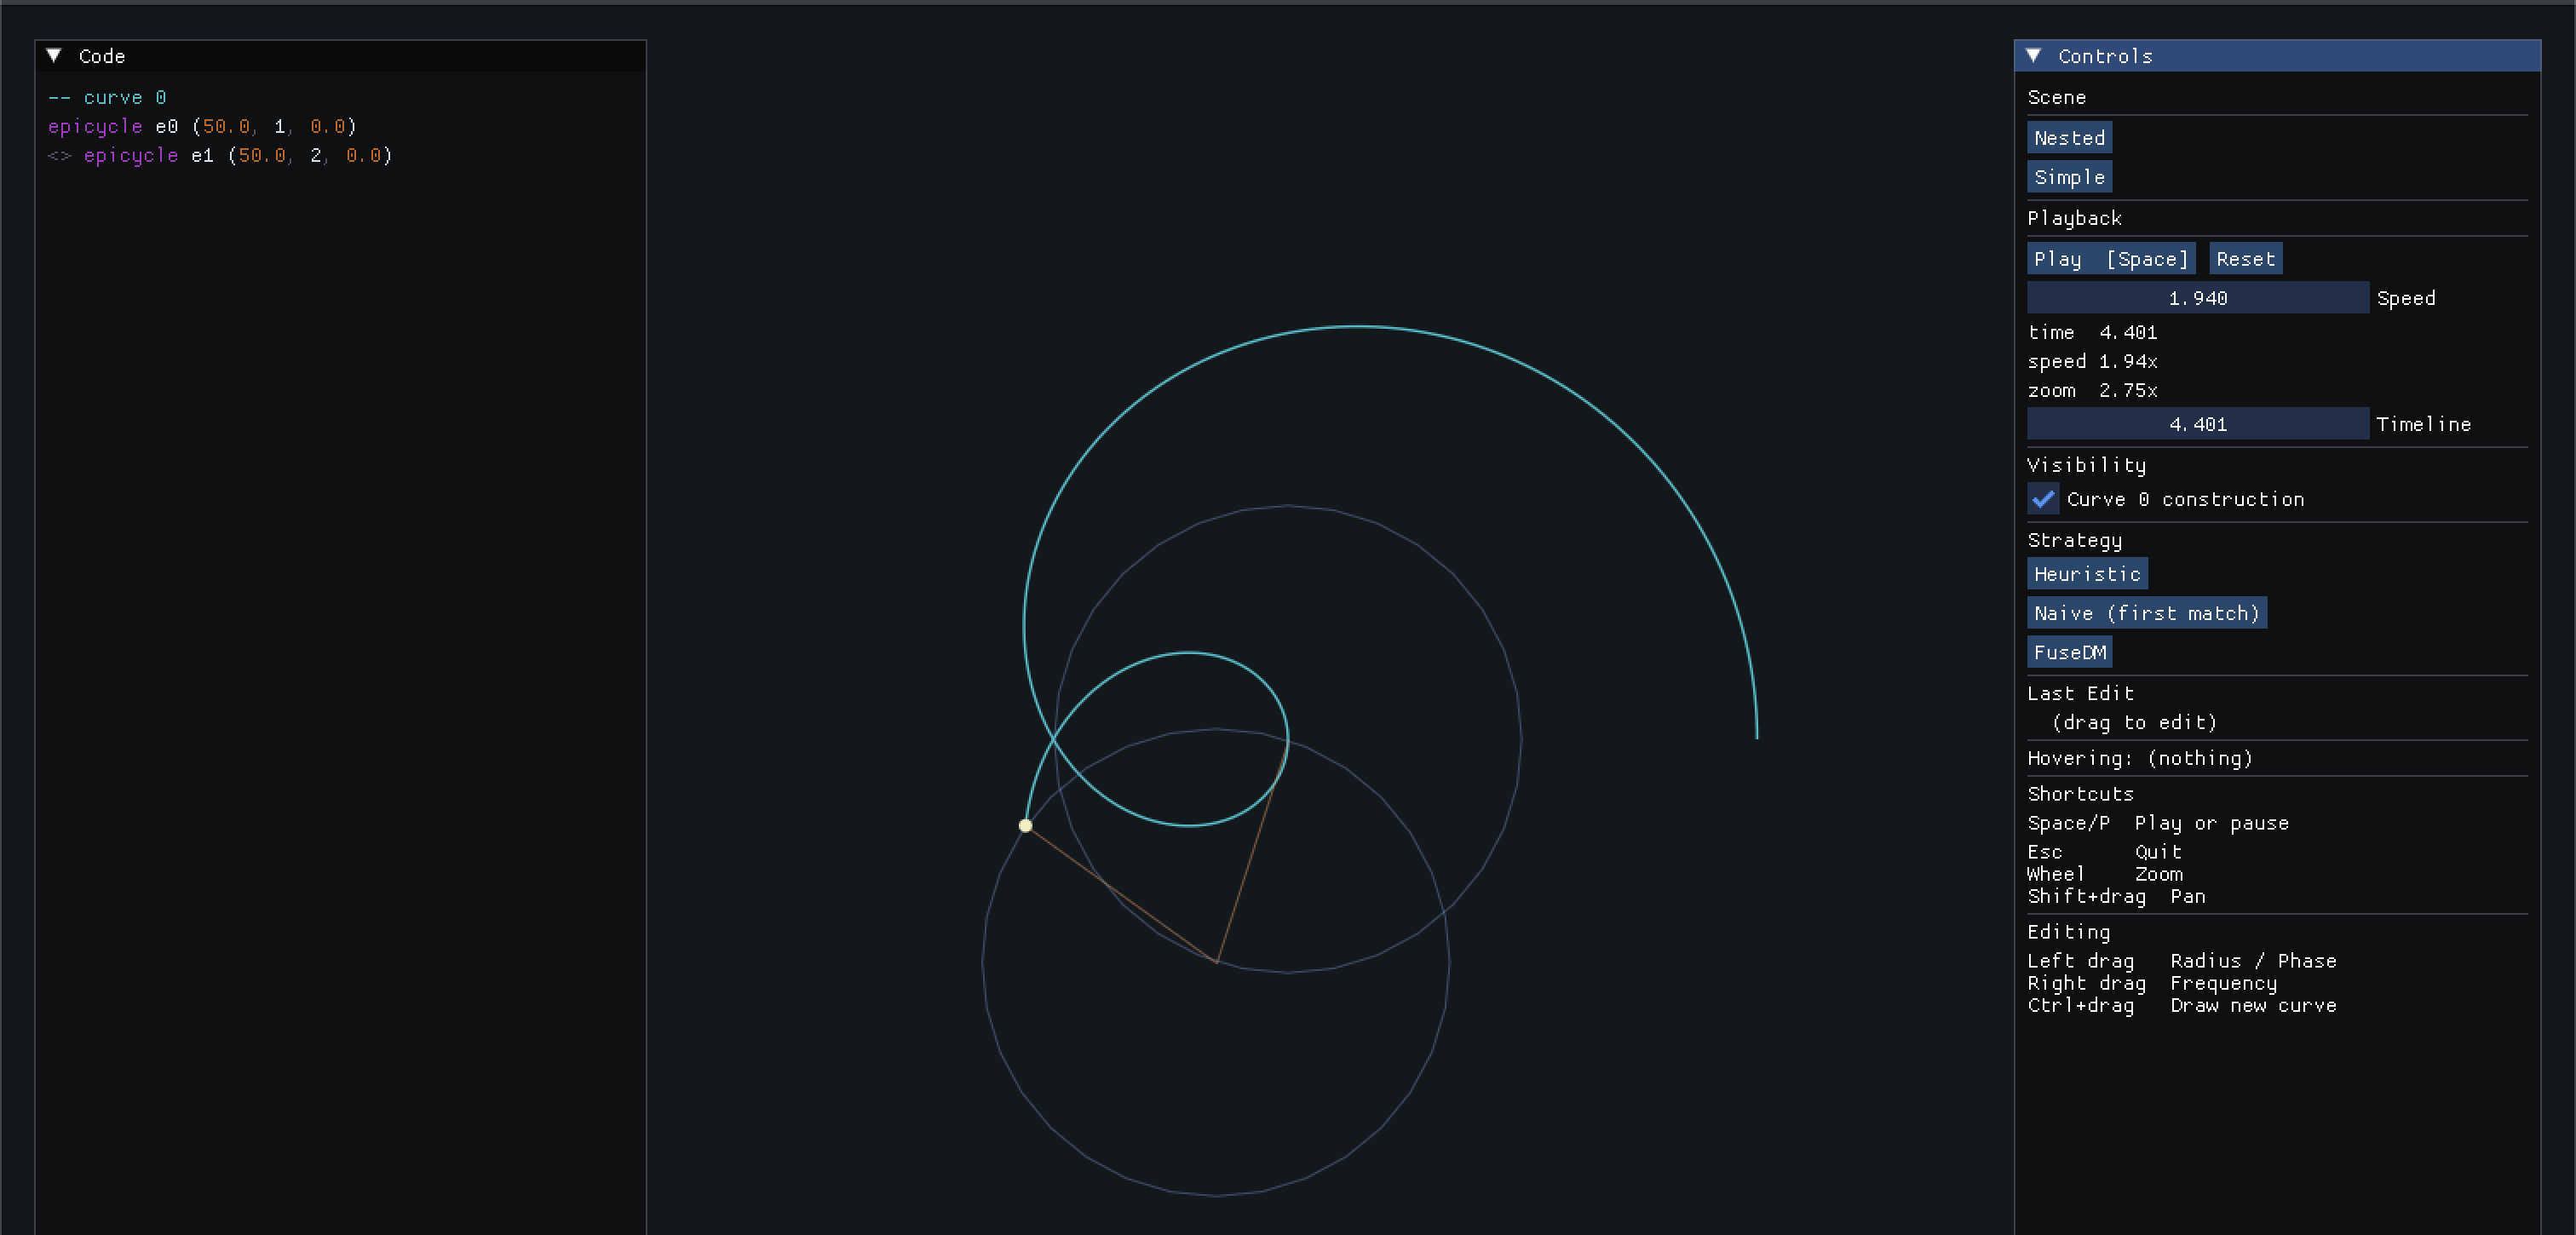
\includegraphics[width=0.8\textwidth]{images/gui-main.png}
	\caption{The main UI of our system, showing the code pane on the left, the rendered curve in the middle, and extra controls on the right.}
	\label{fig:ui}
\end{figure}

\begin{figure}
	\centering
	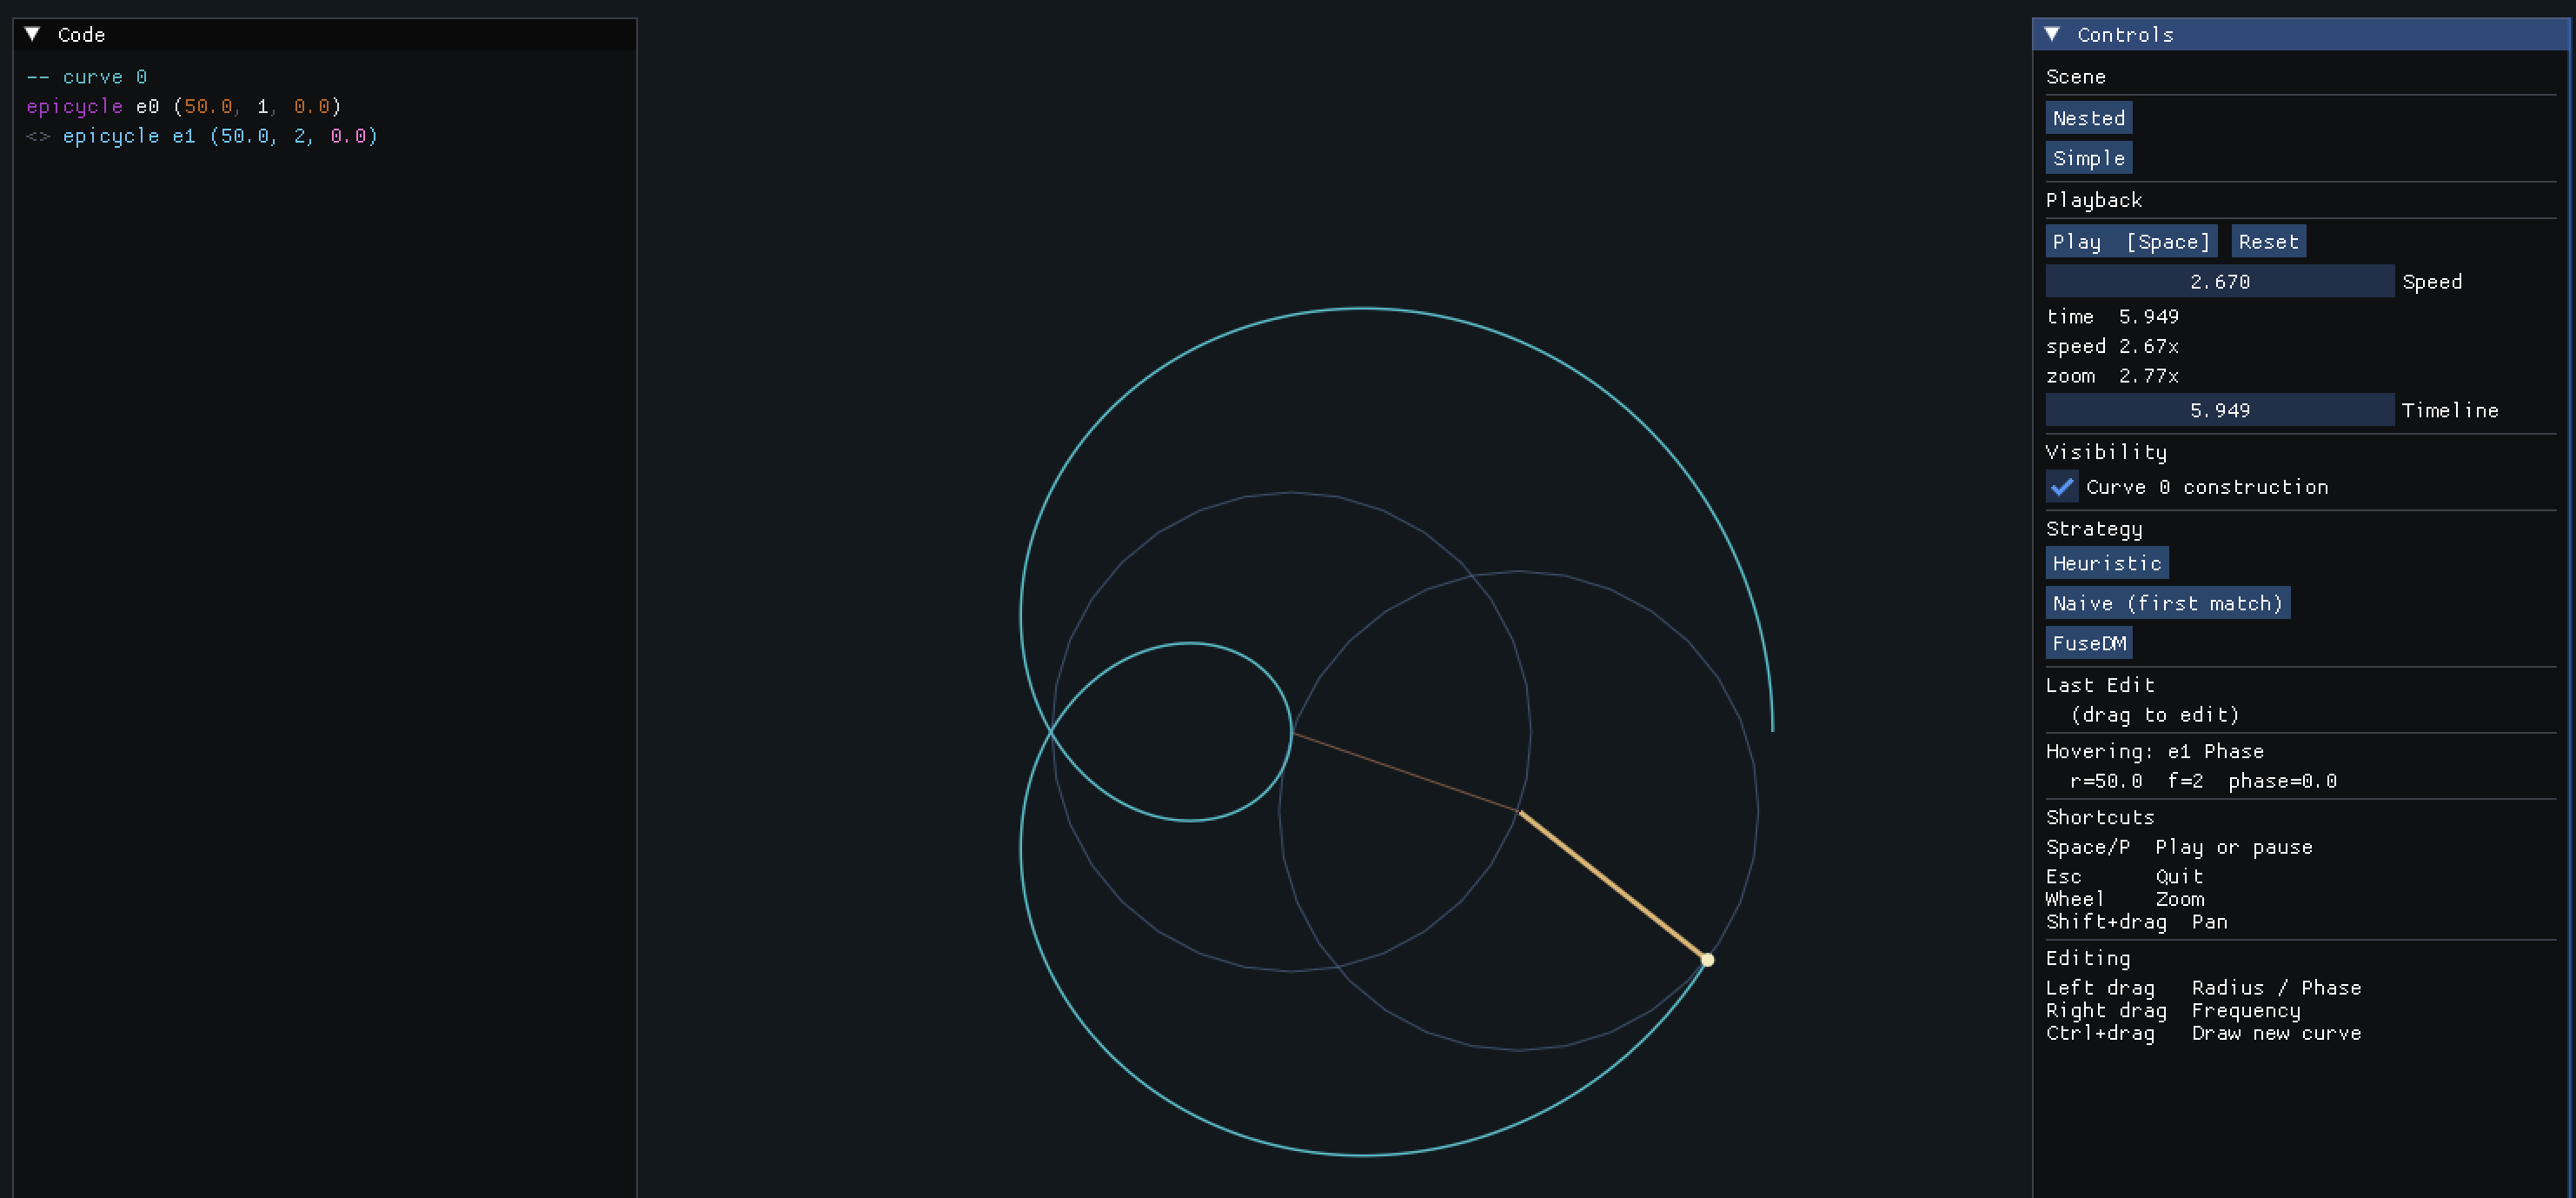
\includegraphics[width=0.8\textwidth]{images/gui-hovering.png}
	\caption{The UI clearly shows the connection between the code and the visual output, highlighting the relevant code and construction element when hovering. In this example, we are hovering over the phase parameter (the arm) of the second epicycle.}
	\label{fig:ui-hover}
\end{figure}


\section{DSL Design}

\subsection{Syntax}

We present the surface syntax of our DSL in Backus-Naur Form (BNF) at a high level.

\begin{bnf}
	$e$ : \text{Expr} ::=
	| $n$ : \text{literal number } ($n \in \mathbb{Q}$)
	| $x$ : \text{parameter or variable } ($x \in \Sigma$)
	| $e_1 + e_2$ : \text{addition}
	| $e_1 \times e_2$                    : \text{multiplication}
	| $e^{-1}$                            : \text{reciprocal}
	| \text{let } $x = e_1$ \text{ in } $o$ : \text{numeric let-binding}
	;;
	$c$ : \text{Curve} ::=
	| $\text{epicycle}(e_r, e_\omega, e_\phi)$ : \text{Epicycle definition}
	| $c_1 \oplus c_2$ : \text{Curve concatenation}
	;;
	$o$ : \text{CurveOrExpr} ::=
	|	$e \mid c$
\end{bnf}

We define our DSL as two separate sub-languages: a language of numeric expressions, and a language of curves. This provides a
clear separation of concerns, simplifying the language for the end user but also simplifying our implementation.

One important design choice is that let-bindings are only allowed to bind numeric values, and not curves. This makes expressions like $\text{let } c = \text{epicycle}(e_r, e_\omega, e_\phi) \text{ in } c \oplus c$ unrepresentable. This prevents geometric aliasing, which causes our DSL to represent a Directed Acyclic Graph (DAG) rather than a strict tree. This would cause backwards solving to become exponentially more complex with far more ambiguous updates.

For similar reasons, our language is deliberately minimal. We include only the minimum viable constructs for a reasonable level of expressivity. The notable omissions of subtraction and division can be derived from the existing constructs.

\subsubsection{Canonicalisation}

From a purely mathematical perspective, a chain of epicycles can be canonicalised: any two epicycles with identical frequencies can be algebraically merged into a single epicycle by combining their radii and phases as complex vectors. However, we reject this in our system -- in the context of bidirectional creative coding, automatically merging structurally distinct AST nodes violates the principle of preserving the programmer's intent. Epicycles may be defined with identical frequencies to logically group sections of source code, or for prototyping. By keeping the AST unadulterated, we maintain an intuitive 1:1 mapping between the source code and visual domain.
We emphasise that this lack of canonicalisation does \textit{not} reintroduce ambiguity into the View-Update problem: because our system exposes the \textit{construction} of the curve rather than just the final trace, the user interaction is always targeted and uniquely identifiable to the exact component epicycle.

\subsection{Statics}

To formalise the statics of our language, we define a closed universe of types available in the DSL. We distinguish between numeric types $\eta$, which may be bound to variables, and the general universe of types $\tau$:

\begin{bnf}
	$\eta$ ::= $\mathbb{Z}$ | $\mathbb{Q}$
	;;
	$\tau$ ::= $\eta$ | \text{Curve}
\end{bnf}

Our statics are defined by the typing relation $\Gamma \vdash e : \tau$, where $\Gamma$ is an environment mapping variables to types.

\begin{mathpar}
	\inferrule*[right=T-LitInt]
	{ n \in \mathbb{Z}  }
	{ \Gamma \vdash n : \mathbb{Z} }

	\inferrule*[right=T-LitRat]
	{ n \in \mathbb{Q}  }
	{ \Gamma \vdash n : \mathbb{Q} }

	\inferrule*[right=T-Var]
	{ x : \tau \in \Gamma}
	{ \Gamma \vdash x : \tau }

	\inferrule*[right=T-Add]
	{ \Gamma \vdash e_1 : \eta \\ \Gamma \vdash e_2 : \eta }
	{ \Gamma \vdash e_1 + e_2 : \eta }

	\inferrule*[right=T-Mult]
	{ \Gamma \vdash e_1 : \eta \\ \Gamma \vdash e_2 : \eta }
	{ \Gamma \vdash e_1 \times e_2 : \eta }

	\inferrule*[right=T-Recip]
	{ \Gamma \vdash e : \eta }
	{ \Gamma \vdash e^{-1} : \eta }

	\inferrule*[right=T-Let]
	{ \Gamma \vdash e_1 : \eta \\ \Gamma, x : \eta \vdash o : \tau}
	{ \Gamma \vdash \text{let } x = e_1 \text{ in } o : \tau }

	\inferrule*[right=T-Epicycle]
	{ \Gamma \vdash e_r : \eta \\ \Gamma \vdash e_\omega : \mathbb{Z} \\ \Gamma \vdash e_\phi : \eta }
	{ \Gamma \vdash \text{epicycle}(e_r, e_\omega, e_\phi) : \text{Curve} }

	\inferrule*[right=T-Concatenate]
	{ \Gamma \vdash c_1 : \text{Curve} \\ \Gamma \vdash c_2 : \text{Curve} }
	{ \Gamma \vdash c_1 \oplus c_2 : \text{Curve} }
\end{mathpar}

\subsubsection{Normal Forms}
\label{sec:normal-form}
The decision to restrict let-bindings to only bind numeric values allows us to define a clear normal form for our DSL. Because curves cannot be bound to variables, no curve expression can ever be nested inside the evaluation scope of a numeric expression.
This leads the language to separate into 3 \textit{non}-mutually recursive layers: purely numeric expressions, variable binders, and curve compositions. Consequently, any valid AST can be partitioned into a Normal Form, where let bindings are `floated' to the root of the program without affecting the evaluation of the expression.


\begin{definition}[Let-Normal Form]

	An expression $P^*$ is in Normal Form when of the form
	\begin{equation*}
		P^* = \text{let } x_1 = e_1 \text{ in let } x_2 = e_2 \text{ in ... let } x_n = e_n \text{ in } C
	\end{equation*}
	where each $e_i$ is a purely numeric \verb|Expr| containing no further \verb|let| bindings, and $C$ is a \verb|Curve|
\end{definition}

\begin{theorem}[Normalisation]

	For any well-typed program $\sigma \vdash P : \text{Curve}$, there exists a program $P^*$ in let-normal form such that $P$ and $P^*$ are semantically equivalent
\end{theorem}

\begin{proof}
	We proceed by structural induction over the syntax of $P$. We first define the floating operation as a transformation that commutes let-bindings outwards of every syntax rule.

	\textbf{Numeric Constructors:} For any binary numeric operation $\odot \in \{+, \times\}$:
	\begin{align*}
		(\text{let } x = e_1 \text{ in } e_2) \odot e_3 & \equiv \text{let } x = e_1 \text{ in } (e_2 \odot e_3) \\
		e_1 \odot (\text{let } x = e_2 \text{ in } e_3) & \equiv \text{let } x = e_2 \text{ in } (e_1 \odot e_3)
	\end{align*}
	A similar rule applies for the unary reciprocal operator which we omit for brevity.

	\textbf{Curve Constructors:} By the \textsc{T-Let} typing rule, variables can only bind numeric types $\eta$. Therefore, a \texttt{let} can never bind a \texttt{Curve}, but may appear inside one of its parameters. We can lift these bindings outward:
	\begin{align*}
		\text{epicycle}(\text{let } x = e_1 \text{ in } e_r, e_\omega, e_\phi) & \equiv \text{let } x = e_1 \text{ in } \text{epicycle}(e_r, e_\omega, e_\phi) \\
		c_1 \oplus (\text{let } x = e_1 \text{ in } o)                         & \equiv \text{let } x = e_1 \text{ in } (c_1 \oplus o)
	\end{align*}
	The cases for other curve parameters $e_\omega$ and $e_\phi$ are similar.

	\textbf{Base Cases:} Literals and variable references cannot contain any \texttt{let} bindings and so are trivially in normal form.

	\textbf{Inductive Case:} For any expression containing a \texttt{let} binding, we repeatedly apply the rewrite rules to push the binding `up` one level of the AST. Because the AST is finite, and the rewrite rules strictly decrease the depth of the \texttt{let} node without duplicating it, this process is guaranteed to terminate.

\end{proof}

\subsection{Expressivity}

This DSL captures finite epicycle chains whose parameters are determined by closed-form first-order arithmetic with let-bindings. Because all terms are closed, every parameter ultimately reduces to a composition of literals through $+$, $\times$, and $^{-1}$, yielding a concrete value at evaluation time.  More formally, the DSL expresses the set of finite trigonometric polynomials of the form
\begin{equation*}
	f(t) = \sum_{k=1}^N c_k \cdot e^{i(\omega_k t + \phi_k)}
\end{equation*}
where each coefficient $c_k \in \mathbb{C}$ is determined by a closed arithmetic expression over $\mathbb{R}$ (or $\mathbb{Z}$ for frequencies).



\subsection{Implementation}

We implement our DSL as a deep embedding in Haskell, using the Embedding by Unembedding approach introduced in \cref{sec:ebu}.

\subsubsection{Type-Level Architecture}

The bipartite type system we have defined is somewhat difficult to express cleanly in Haskell. Typically when embedding DSLs, we index the type of each expression by some type variable: for example \verb|data AST env a where ...|. This however presents issues with implementing our \textsc{T-Let} rule, constraining the type of the bound variable to be a numeric type. We might think to use a custom type class constraint:
\begin{minted}{haskell}
	-- | Bind a variable 
	Let :: (BindableNum n) => AST env n -> AST (n : env) a -> AST env a
	-- | Concatenate two curves
	Append :: AST env Curve -> AST env Curve -> AST env Curve
\end{minted}
However, Haskell adopts an ``open-world'' approach to type classes. We cannot assume that \verb|instance BindableNum Curve| won't be defined in the future. This design forces us to write partial functions: some function which evaluates numeric expressions\begin{minted}{haskell}
	evalExpr :: (BindableNum n) => AST env n -> n
\end{minted}
still requires including an unsafe case
\begin{verbatim}
evalExpr (Append a b) = error "unreachable"
\end{verbatim}


To ameliorate this, we define a closed-world of \textit{kinds}. Kinds allow categorisation of types, just as types categorise values. For example in Haskell, we say that \verb|Int :: Type|, \verb|Maybe :: Type -> Type|, etc. In the above example, \verb|a :: Type|, which is problematic because it gives no guarantees about the specific types that are allowed. We use GHC's \verb|TypeData| extension to define a new kind \verb|ASTSort|:
\begin{minted}{haskell}
{-# LANGUAGE TypeData #-}
type data ASTSort = SNum Type | SCurve
\end{minted}
We can then index our AST by this new kind:
\begin{minted}{haskell}
data AST env (a :: ASTSort) where
  Let :: (BindableNum n) => AST env (SNum n) -> AST (SNum n : env) a -> AST env a
  Append :: AST env SCurve -> AST env SCurve -> AST env SCurve
\end{minted}

To bridge the gap between \verb|ASTSort| and runtime values, we use the \textit{singleton pattern}. We define a GADT \verb|SortVal|, which serves as a term-level witness for the \verb|ASTSort| kind:

\begin{minted}{haskell}
data SortVal (s :: ASTSort) where
  VNum   :: n -> SortVal (SNum n)
  VCurve :: Curve -> SortVal SCurve
\end{minted}

This establishes a strict 1:1 correspondence between the type-level index and the term-level value. If the index is \verb|SNum n|, the runtime value is structurally guaranteed to be \verb|VNum|, which follows the same logic for \verb|SCurve| and \verb|VCurve|.

By populating our environment with these singletons (\verb|type IEnv = Env SortVal|), pattern matching on the environment yields type equality proofs directly to the compiler.

The type signature for the evaluator now becomes \verb|evalExpr :: AST env (SNum n) -> n|. Because \verb|ASTSort| is closed, GHC can prove that the \verb|SCurve| kind returned by \verb|Append| will never unify with \verb|SNum|, satisfying the exhaustive pattern matching checking without needing explicit unsafe cases.

We still use the \verb|BindableNum| class, which remains necessary but serves a distinct purpose: While \verb|ASTSort| structurally isolates the AST branches, \verb|BindableNum| enforces compile-time constraints, ensuring that nonsensical type combinations (such as attempting to construct an AST node for \verb|SNum String|) are impossible to construct.

However, one partial case remains: \verb|Param|. Although we guarantee \textit{within} our DSL that only numeric types can be bound, there is nothing stopping an expression being defined that references a free variable of type \verb|SCurve|:
\begin{minted}{haskell}
badExpression :: AST '[SCurve] SCurve
badExpression = Param IZ
\end{minted}

\subsubsection{Trees That Grow}
When dealing with Abstract Syntax Trees it is often beneficial to have multiple \textit{stages} of the AST, where each stage has different invariants, or is annotated with extra information. Indeed, for our system, we have two main stages: the initial ``parsed'' AST, and a second, where every \texttt{epicycle} is annotated with a unique identifier. We use the \textit{Trees that Grow}\cite{najd_trees_2016} approach to re-use the same AST definition for both stages. This is done by adding an extra type level index to the AST, denoting the stage of the AST, and then using \textit{type families} to define different types for each stage. For the unique identifiers, we define the types like so:
\begin{minted}{haskell}
-- | Marker for the AST's stage
type data Stage 
  = Parsed -- ^ the initial AST, converted from HOAS
  | Numbered -- ^ the AST after numbering

-- | Type family for epicycle "eXtensions"
type family XEpicycle (p :: Stage) where
-- the initial AST has no extra information
  XEpicycle Parsed = () 
  -- the numbered AST has an extra EpicycleId field
  XEpicycle Numbered = EpicycleId 


data AST (x :: Stage) (env :: [ASTSort]) (s :: ASTSort) where
  -- | Define an epicycle with radius, frequency, and phase
  Epicycle :: 
    XEpicycle x -- ^ extension field
    -> AST x env (SNum Rational) -- ^ radius
    -> AST x env (SNum Int) -- ^ frequency
    -> AST x env (SNum Rational) -- ^ phase
    -> AST x env SCurve
\end{minted}


We also note that the Trees that Grow approach is not only for \textit{adding} data, but also \textit{removing} it. Indeed, this is the main way in which we enforce the constraint that curves cannot be bound to variables. By making a type family which maps some stages to \verb|Void| (the uninhabited type), we guarantee that ASTs of this pattern cannot be constructed:

\begin{minted}{haskell}
type family XParam (s :: ASTSort) where
  XParam SCurve = Void 
  XParam (SNum n) = ()

data AST (x :: Stage) (env :: [ASTSort]) (s :: ASTSort) where
  -- | Reference a variable / parameter from the environment
  Param_ :: (XParam s) -> Ix env s -> AST x env s
  -- ...
\end{minted}

This effectively makes it impossible to write an expression which references a variable of type \verb|SCurve|, and solves the previous problem -- even if we have a free variable of type \verb|SCurve| in our environment, we cannot write an expression which references it, so it cannot affect our semantics.

We also define a \textit{Pattern Synonym} for the \verb|Param_| constructor, to hide this implementation detail from the rest of the codebase:
\begin{minted}{haskell}
pattern Param :: (XParam s ~ ()) => Ix env s -> AST x env s
pattern Param ix = Param_ () ix
{-# COMPLETE Lit, Param, Add, Mul, Recip, Epicycle, Append, Let #-}
\end{minted}

\subsubsection{Adding constraints to Embedding-by-Unembedding}

To make this invalid state unrepresentable with Trees that Grow, we had to fork the \verb|embedding-by-unembedding| library to relax its requirements of \textit{parametricity}. \citeauthor{matsuda_embedding_2023}'s work relies on a common interface that is able to ``lift semantics of variables into semantics of terms'' -- in other words, the \textit{Embedding by Unembedding} approach relies on being able to reference variables in our semantics. This is how the library achieves the seamless conversion from HOAS to De-Bruijn indexed syntax. Specifically, this is done with the \verb|LiftVariables| type class\footnote{A minor deviation from the original paper published to the reference implementation at \url{https://github.com/kztk-m/EbU}}, which defines a function \verb|liftVar :: Var sem env a -> sem env a| for an associated type family \verb|Var|. Importantly, this function is required to be parametric in \verb|a|, so we cannot write a case for \verb|SCurve| or block it without violating parametricity. We make a small tweak to the library to work around this, adding an extra associated type family \verb|LiftConstraint sem (a :: k) :: Constraint|, utilising GHC's \verb|ConstraintKinds| extension. We then redefine
\begin{minted}{haskell}
liftVar :: (LiftConstraint sem a) => Var sem env a -> sem env a
\end{minted}

We can then define $\texttt{LiftConstraint AST}_s = \texttt{XParam Parsed}_s \sim ()$, to enforce that only numeric types can be lifted into the semantics.

The implementation of this change is short but worth discussion. The \verb|unembedding| library evaluates higher-order syntax by performing structural induction over the environment using a type \verb|TEnv|, essentially a list of \verb|Proxy| types. Since \verb|Proxy| carries no information, it does not carry any evidence of the \verb|LiftConstraint| constraint. We expanded the library's existing \verb|OfLength| type to also carry the constraint evidence, and used that in place of \verb|TEnv| throughout the library.

The rest of the changes were minor and mechanical, replacing \verb|TEnv| with \verb|OfLength| and adding the necessary \verb|LiftConstraint| constraints to the type signatures of the various functions that manipulate the environment, and occasionally converting between \verb|OfLength| and \verb|TEnv| when necessary.

The main trade-off of this approach is that the conversion from HOAS to De-Bruijn syntax has a more complex type signature, and so requires some manual type annotations to aid inference. We have not observed any other significant downsides, and argue that this change maintains the library's original design goals while allowing us to enforce the necessary constraints for our DSL.

\subsubsection{Final Implementation}

We present the frontend HOAS interface for our DSL, which is what user code is written in. The De-Bruijn indexed AST implementation can be found in the accompanying codebase.

\begin{minted}{haskell}
type data ASTSort = SNum Type | SCurve

data SortVal (s :: ASTSort) where
  VNum :: n -> SortVal (SNum n)
  VCurve :: Curve -> SortVal SCurve

class Expr (e :: ASTSort -> Type) where
  lit :: (BindableNum n) => n -> e (SNum n)
  add :: (BindableNum n) => e (SNum n) -> e (SNum n) -> e (SNum n)
  mul :: (BindableNum n) => e (SNum n) -> e (SNum n) -> e (SNum n)
  recip :: (BindableNum n, Fractional n) => e (SNum n) -> e (SNum n)
  let_ :: (Typeable n, BindableNum n) => e (SNum n) -> (e (SNum n) -> e a) -> e a

class (Expr e) => CurveExpr e where
  epicycle :: e (SNum Rational) -> e (SNum Int) -> e (SNum Rational) -> e SCurve
  cappend :: e SCurve -> e SCurve -> e SCurve
\end{minted}

Each function cleanly maps to part of the syntax of our language, enforcing the statics using type classes and the aformentioned type-level architecture. The \verb|Typeable| constraint is required for bidirectional semantics to compare ASTs, which we will revisit later.

We can now present a complete example of a curve defined in our DSL, which draws a simple shape:
\begin{minted}{haskell}
curveSimple :: (CurveExpr e) => e SCurve
curveSimple =
    epicycle 120 1 0
        <> epicycle 60 3 0
        <> epicycle 30 5 0
\end{minted}

Note the use of the general \textit{semigroup} operator \verb|<>|, which we overload as an alias of \verb|cappend|.
The graphical output of this is presented in \cref{fig:simple-demo-output}.

\begin{figure}[t]
	\centering
	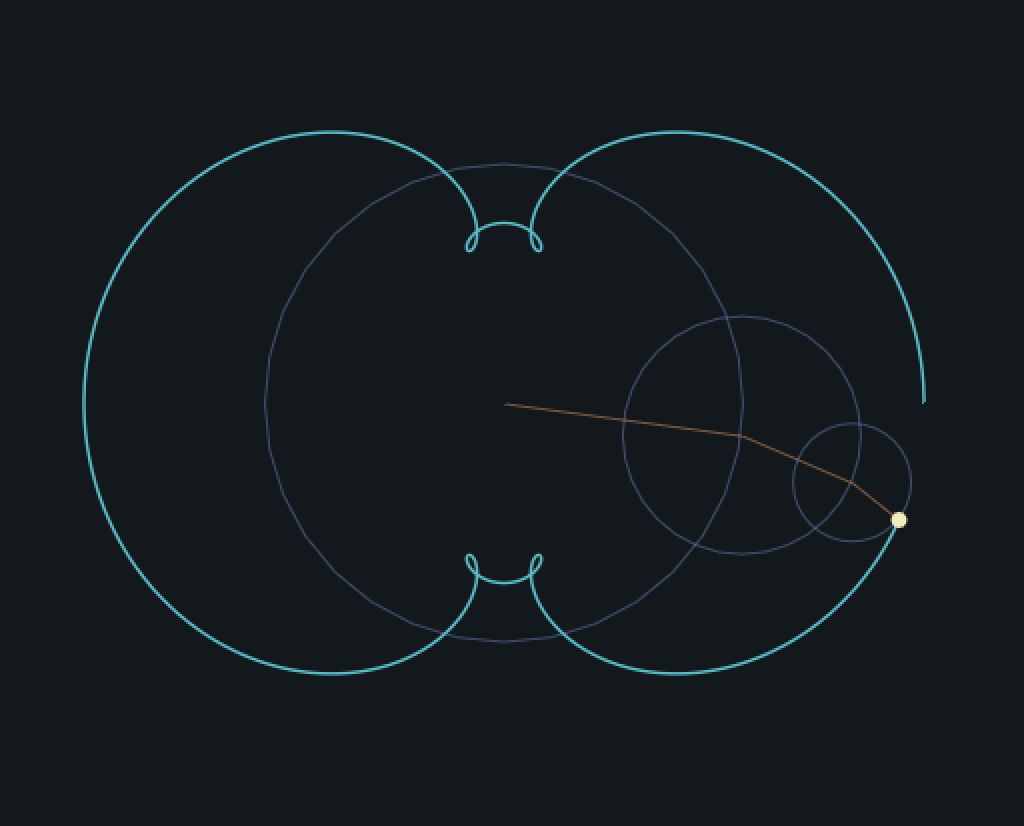
\includegraphics[width=0.5\textwidth]{images/vector-dsl-simple-demo.png}
	\caption{The output of an example curve defined in our DSL.}
	\label{fig:simple-demo-output}
\end{figure}

Our DSL's final design shows a clear correspondence between our described syntax and statics, and the real Haskell code. This is one of the main benefits of embedding DSLs -- rather than just implementing our language, we \textit{encode} it:
\begin{itemize}
	\item $\eta \subset \mathtt{SNum Type}$ \footnote{As types like \texttt{SNum String} are legal to construct, but cannot be used in practice, we cannot say that the two are truly isomorphic}
	\item $\tau \subset \mathtt{ASTSort}$
	\item $\Gamma \cong$ \verb|env :: [ASTSort]|
	\item $x : \tau \in \Gamma \cong$ \verb|Ix env s|
	\item $\Gamma \vdash e : \tau \cong$ \verb|Expr e => e env s|
\end{itemize}


\section{Semantics}

We have discussed the statics and frontend implementation of our DSL, but have not yet covered the semantics. Our implementation aims to evaluate and compare different bidirectional semantics, and so we do not commit to a single \textit{backwards} semantics in this section, however for the most part, the forwards semantics do not vary.

It is useful to abstract the problem domain into a pure data model -- while the domain is visual, interactive, and geometric, we can simplify this into a pure data view. To do this, we introduce a semantic visual projection, implemented as the type \verb|VisualScene|. Rather than directly rendering the AST, we define a forward mapping that flattens the hierarchical, algebraic structure of the AST into a purely geometric snapshot of the curve at a given time $t$.

This type acts as a \textit{view model}, separating concerns between the bidirectional semantics, and the graphical user interface. The forward semantics translate the epicyclic structure into a simpler flat system of coordinates, which isolates the backwards semantics from the rendering engine. In other words, the bidirectional execution code is entirely agnostic to how curves are rendered on a screen and interact with user input.

We take a similar approach to handling user input: when a user manipulates a graphical curve, rather than directly update the AST, we produce a \verb|SceneEdit| value which references a uniquely identified epicycle, along with the target change.



\subsection{Forward Evaluation}\label{sec:eval}


We first present a general big-step semantics for our DSL -- our evaluation has no recursion, state, or control flow, so small-step would not give any more insight.

We define our semantics in terms of a judgement $\sigma, t \vdash e : \tau \Downarrow v$, meaning under environment $\sigma$ at time $t$, expression $e$ with type $\tau$ evaluates to value $v$. The numeric part of our language does not depend on $t$, unlike the curve part, but is included for uniformity.

\begin{mathpar}
	\inferrule*[right=E-LitInt]
	{ }
	{ \sigma, t \vdash n : \mathbb{Z} \Downarrow n }

	\inferrule*[right=E-LitRat]
	{ }
	{ \sigma, t \vdash n : \mathbb{Q} \Downarrow n }

	\inferrule*[right=E-Var]
	{ x : \tau \in \sigma }
	{ \sigma, t \vdash x : \tau \Downarrow \sigma(x) }

	\inferrule*[right=E-Add]
	{ \sigma, t \vdash e_1 : \eta \Downarrow v_1 \\ \sigma, t \vdash e_2 : \eta \Downarrow v_2 }
	{ \sigma, t \vdash e_1 + e_2 : \eta \Downarrow v_1 + v_2 }

	\inferrule*[right=E-Mult]
	{ \sigma, t \vdash e_1 : \eta \Downarrow v_1 \\ \sigma, t \vdash e_2 : \eta \Downarrow v_2 }
	{ \sigma, t \vdash e_1 \times e_2 : \eta \Downarrow v_1 \times v_2 }

	\inferrule*[right=E-Recip]
	{ \sigma, t \vdash e : \mathbb{Q} \Downarrow v }
	{ \sigma, t \vdash e^{-1} : \mathbb{Q} \Downarrow \frac{1}{v} }

	\inferrule*[right=E-Let]
	{ \sigma, t \vdash e_1 : \eta \Downarrow v_1 \\ \sigma[x \mapsto v_1], t \vdash o : \tau \Downarrow v }
	{ \sigma, t \vdash \text{let } x = e_1 \text{ in } o : \tau \Downarrow v }


	\inferrule*[right=C-Epicycle]
	{ \sigma, t \vdash e_r : \mathbb{Q} \Downarrow v_r \\ \sigma, t \vdash e_\omega : \mathbb{Z} \Downarrow v_\omega \\ \sigma, t \vdash e_\phi : \mathbb{Q} \Downarrow v_\phi }
	{ \sigma, t \vdash \text{epicycle}(e_r, e_\omega, e_\phi) : \text{Curve} \Downarrow v_r \cdot e^{i(v_\omega \cdot t + v_\phi)} }

	\inferrule*[right=C-Append]
	{ \sigma, t \vdash c_1 : \text{Curve} \Downarrow v_1 \\ \sigma, t \vdash c_2 : \text{Curve} \Downarrow v_2 }
	{ \sigma, t \vdash c_1 \oplus c_2 : \text{Curve} \Downarrow v_1 + v_2 }
\end{mathpar}

\subsection{Backward Evaluation Framework}

One of the main goals of this project is to evaluate and compare multiple different approaches to bidirectional semantics. We will now introduce what this means in general, and then present the specific approaches we have implemented.

Just as we have a forward evaluation relation $\Downarrow$, we also have a backward evaluation relation $\Uparrow$. This relation is more complex than the forward relation, as it has to update both the expression and the environment. We define the general judgement as $\sigma, t \vdash e : \tau \Uparrow v' \rightsquigarrow (\sigma', e')$, meaning that for expression $e : \tau$ under environment $\sigma$ at time $t$, to update the value to $v'$, we can produce an updated environment $\sigma'$ and an updated expression $e'$. In other words, this relation defines a `solution' to $e, \sigma$ for some $v'$, such that $\sigma', t \vdash e' : \tau \Downarrow v'$.

This leads to a few properties we would like to hold for our semantics:

\textbf{PutGet} (correctness): If backwards evaluation produces an update, re-evaluating the result yields the target value:
\begin{mathpar}
	\inferrule*[right=PutGet]
	{ \sigma, t \vdash e : \tau \Uparrow v' \rightsquigarrow (\sigma', e') }
	{ \sigma', t \vdash e' : \tau \Downarrow v' }
\end{mathpar}

\textbf{GetPut} (stability): Updating to the current value produces no change:
\begin{mathpar}
	\inferrule*[right=GetPut]
	{ \sigma, t \vdash e : \tau \Downarrow v \\ \sigma, t \vdash e : \tau \Uparrow v \rightsquigarrow (\sigma', e') }
	{ \sigma' = \sigma \\ e' = e }
\end{mathpar}

\textbf{PutPut} (consistency): If we update to a value, then update again to a new value, this is the same as just updating to the new value:
\begin{mathpar}
	\inferrule*[right=PutPut]
	{ \sigma, t \vdash e : \tau \Uparrow v' \rightsquigarrow (\sigma', e') \\ \sigma', t \vdash e' : \tau \Uparrow v'' \rightsquigarrow (\sigma'', e'') }
	{ \sigma, t \vdash e : \tau \Uparrow v'' \rightsquigarrow (\sigma'', e'') }
\end{mathpar}

The \textbf{PutPut} property is a generalisation of a looser property of \textit{convergence}: if we update to a value, then update again to the same value, this is the same as just updating to that value. This is essentially a stability property of the backwards semantics, and is very important for the user experience: if the user drags a curve to a new position, and then holds it there, the curve should not start `drifting' around as the backwards semantics continue.

Defining the backwards semantics is the main technical challenge of this project, and the field of bidirectional programming as a whole. One challenge is the introduction of \textit{nondeterminism}. In the forward direction, most semantics are deterministic -- every expression will evaluate to a single, unique value.

In the context of our language, we observe that while the backwards judgement operates over the entire AST, there is a clear separation of concerns between the numeric and curve parts of the language. At the curve level, our numbering pass assigns each \verb|epicycle| node a unique identifier and thus the backwards mapping is fully deterministic: within $\text{epicycle}(e_r, e_\omega, e_\phi)$, an update to one of its parameters targets exactly one of the three sub-expressions.
All non-determinism therefore is confined exclusively to the numeric part of the language. For an expression $e$ with $k$ parameter leaves (\verb|Param| nodes), we define the candidate set $\mathcal{C}(e, \sigma, v')$ as the set of all environment updates $\sigma'$ such that $\sigma', t \vdash e : \tau \Downarrow v'$. Then:
\begin{itemize}
	\item \textbf{Literals} yield $|\mathcal{C}| = 0$ if $n \neq v'$, and $|\mathcal{C}| = 1$ if $n = v'$.
	\item \textbf{Parameters} yield $|\mathcal{C}| = 1$: set $\sigma'(x) = v'$
	\item \textbf{Recip} yields $|\mathcal{C}| = 1$: solve uniquely for $e_1$ as $v_1' = 1/v'$
\end{itemize}

The compound expressions are where nondeterminism appears:
\begin{itemize}
	\item \textbf{Add} $e_1 + e_2 = v'$ admits the candidate set $\mathcal{C} = \{ (v' - v_2, v_2) | v_2 \in \mathbb{R} \}$. We will resolve this infinite set in various ways in our different semantics, which constrain the search space to a finite set.
	\item \textbf{Mul} is similar, with the extra case of $v_1 = 0$ or $v_2 = 0$ requiring special treatment
\end{itemize}

In contrast, the \verb|Let| construct introduces an entirely different kind of non-determinism: rather than algebraic ambiguity, we have \textit{aliasing}. Consider
\begin{equation*}
	\text{let } r = 10 \text { in epicycle}(r, 1, 0) \oplus \text{epicycle}(r, 3, 0)
\end{equation*}
A backward update targeting the first epicycle's radius to 12 produces two distinct update candidates: update the bound variable $r$ to 12, propagating the change to both epicycles, or rewrite the AST to break the sharing, and introduce a new variable or constant multiplier to only update the first epicycle. Unlike the numeric cases, these two candidates are structurally and \textit{semantically} distinct. The candidate set for \verb|Let| is bounded by the number of usage sites of the bound variable, but the impact of each choice is global.

This characterisation is a direct consequence of domain restriction. In a general-purpose language, the ambiguity space is unbounded: arbitrary control flow, functions, and complex combinators make the candidate set infinite and unstructured. In our DSL, we are able to keep the candidate set finite in many cases, pushing the non-determinism to a manageable level.

\section{Non-Deterministic Semantics}
\label{sec:non-deterministic-semantics}
The first bidirectional semantics we investigate is a heuristic approach, proposed by \citeauthor{mayer_bidirectional_2018} as an improvement over the original trace-based Sketch-n-Sketch semantics\cite{chugh_programmatic_2016}. This defines an inherently non-deterministic backwards semantics, and defers the resolution of this to some external heuristic -- in their case, asking the user to choose from a small set of candidates. In our case, we instead resolve the ambiguity by defining a heuristic function. As previously discussed, our DSL is significantly simpler than the \textit{LittleLeo} language used in the paper, so we redefine their semantics in our context, noting that the majority of the complex cases are no longer present.

For consistency, we continue to use our judgement notation.  Our judgement form $\sigma, t \vdash e : \tau \Downarrow v$ translates to $(E \vdash e) \Rightarrow v$, and $\sigma, t \vdash e : \tau \Uparrow v' \rightsquigarrow (\sigma', e')$ translates to $(E \vdash e) \Leftarrow v' \rightsquigarrow (E' \vdash e')$ by \citeauthor{mayer_bidirectional_2018}. Some extra differences worth noting are that our environments are type-indexed, and we use De-Bruijn indices to avoid having to manually pattern match over environments in rules like \textsc{U-Var}\footnote{Variable names are used throughout judgements for clarity}. For this semantics, the forward evaluation is the same as the standard semantics defined in \cref{sec:eval}, but with our new backwards evaluation defined as follows:

\begin{mathpar}
	\inferrule*[right=U-Const]
	{ }
	{ \sigma \vdash n : \eta \Uparrow n' \rightsquigarrow (\sigma, n') }

	\inferrule*[right=U-Var]
	{ }
	{ \sigma \vdash x : \tau \Uparrow v' \rightsquigarrow (\sigma[x \mapsto v'], x)}

	\inferrule*[right=U-Add-1]
	{ \sigma \vdash e_2 : \eta \Downarrow v_2 \\ \sigma \vdash e_1 : \eta \Uparrow v' - v_2 \rightsquigarrow (\sigma_1, e_1')  }
	{ \sigma \vdash e_1 + e_2 : \eta \Uparrow v' \rightsquigarrow (\sigma_1, e_1' + e_2) }

	\inferrule*[right=U-Add-2]
	{ \sigma \vdash e_1 : \eta \Downarrow v_1 \\ \sigma \vdash e_2 : \eta \Uparrow v' - v_1 \rightsquigarrow (\sigma_2, e_2') }
	{ \sigma \vdash e_1 + e_2 : \eta \Uparrow v' \rightsquigarrow (\sigma_2, e_1 + e_2') }

	\inferrule*[right=U-Mul-1]
	{\sigma \vdash e_2 : \eta \Downarrow v_2
		\\ v_2 \neq 0
		\\ v' / v_2 \in \eta
		\\  \sigma \vdash e_1 : \eta \Uparrow v' / v_2 \rightsquigarrow (\sigma_1, e_1') }
	{ \sigma \vdash e_1 \times e_2 : \eta \Uparrow v' \rightsquigarrow (\sigma_1, e_1' \times e_2) }

	\inferrule*[right=U-Mul-2]
	{ \sigma \vdash e_1 : \eta \Downarrow v_1
		\\ v_1 \neq 0
		\\ v' / v_1 \in \eta
		\\ \sigma \vdash e_2 : \eta \Uparrow v' / v_1 \rightsquigarrow (\sigma_2, e_2') }
	{ \sigma \vdash e_1 \times e_2 : \eta \Uparrow v' \rightsquigarrow (\sigma_2, e_1 \times e_2') }

	\inferrule*[right=U-Recip]
	{ \sigma \vdash e : \mathbb{Q} \Uparrow 1/v' \rightsquigarrow (\sigma', e') }
	{ \sigma \vdash e^{-1} : \mathbb{Q} \Uparrow v' \rightsquigarrow (\sigma', e'^{-1}) }

	\inferrule*[right=U-Let]
	{ \sigma \vdash e_1 : \eta \Downarrow v_1
		\\ \sigma[x \mapsto v_1] \vdash o : \tau \Uparrow v' \rightsquigarrow (\sigma_\text{outer}[x \mapsto v_1'], o')
		\\ \sigma_\text{outer} \vdash e_1 : \eta \Uparrow v_1' \rightsquigarrow (\sigma', e_1') }
	{ \sigma \vdash \text{let } x = e_1 \text{ in } o : \tau \Uparrow v' \rightsquigarrow (\sigma', \text{let } x = e_1' \text{ in } o') }
\end{mathpar}

We omit the trivial cases for \verb|epicycle| and $\oplus$ for brevity.

As mentioned, these semantics are non-deterministic. The rules \textsc{U-Add-1} and \textsc{U-Add-2} both match for the same expression, but produce different updates. The same is true for \textsc{U-Mul-1} and \textsc{U-Mul-2}. Due to our frequency domain being $\mathbb{Z}$, we also include checks that candidate updates are valid for this domain. This also has the added benefit of acting as a natural pruning mechanism, keeping the candidate small by filtering out invalid updates.

Aside from making edge cases more explicit, simplification, and adjustment to our specific language, these rules are virtually identical to the ones defined by \citeauthor{mayer_bidirectional_2018}, with the major exception of the \textsc{U-Let} rule. The original paper's semantics propagates the update through both variables independently, and then resolves conflicts separately through the use of an ``environment merge operation'' $E_1 \prescript{e_1}{}{\oplus^{e_2}} E_2$, which reconciles the two candidate environments in the case they diverge.
In contrast, we choose to evaluate the two sub-updates sequentially rather than non-deterministically, avoiding the need for this environment merge. This would violate the PutGet property, which we guard against by adding an extra check after construction, filtering out cases where PutGet would fail \textit{specifically} because of sequential threading. This is practical because our candidate set is small and finite thanks to the domain restriction of our language; in the paper's general setting, this approach would be infeasible.

To resolve the non-determinism, we define a cost model that ranks candidates by how ``invasive'' the edit is to the original program. We define an \textbf{edit depth} ordering:
\begin{equation*}
	\text{NoEdit} < \text{LitEdit} < \text{LocalParam} < \text{OuterParam}(n) < \text{ImpossibleEdit}
\end{equation*} with the following intuitive meaning:
\begin{itemize}
	\item \textbf{NoEdit} means the candidate is the same as the original
	\item \textbf{LitEdit} means only a literal was changed
	\item \textbf{LocalParam} means a parameter in the innermost scope was changed
	\item \textbf{OuterParam}$(n)$ means a parameter $n$ scopes out was changed
	\item \textbf{ImpossibleEdit} means the edit depth could not be determined (e.g. when comparing two structurally different ASTs)
\end{itemize}

This ordering captures the intuition that edits closer to the point of use are preferred over edits that propagate through variable binding, essentially trying to make edits as `local' as possible. We take this approach to try and make edits more predictable to the user -- an edit with a lower edit depth is generally more desirable than one with a higher edit depth. This is an opinionated, but principled design decision we will evaluate later, based on the assumption that the user probably wants to change the thing they are clicking on \textit{without} altering everything else.
Our heuristic strategy then evaluates all possible backwards updates, and selects the candidate with the minimum edit depth.

We implement the non-determinism backwards rules using Haskell's \verb|List| monad, which elegantly models non-deterministic computation: each rule returns a list of candidates, and the monadic bind operator composes these choices. The edit depth is computed by a structural comparison function \verb|diffExpr| that traverses two ASTs in parallel, returning the most invasive edit encountered. This is where the \verb|Typeable| constraint on \verb|Let| is required -- we can only compare two \verb|Let| nodes if their binders are of the same type, otherwise we fall back to ImpossibleEdit. Importantly, when evaluating multiple branches such as for an \verb|Add| node, we take the maximum edit depth from either branch, rather than the sum. This choice is justified by the branching nature of our update semantics. Each branch rule updates \textit{either} operand independently, and never both simultaneously. Therefore, any single candidate updates up to one leaf node, and so we use the \verb|max| combinator to propagate this cost up through the tree. This ranking is also intuitive -- the `danger' of an edit is determined by the most invasive change it makes, rather than the total number of changes; which would also remain useful if future extensions to the semantics permitted composite edits.

We define two main strategies with this algorithm as a base: a \textbf{naive update}, which simply applies the first candidate returned by the backwards semantics, and a \textbf{heuristic update}, which applies the minimum edit depth candidate.


\section{Delta-Based Semantics}

In \cref{sec:edit-lenses} we introduced the idea of an \textit{edit lens}. As discussed, lenses struggle to handle the presence of shared bindings, however, the \textit{delta-based} approach to edit lenses bears further investigation. \citeauthor{zhang_fusing_2024} propose a new general purpose delta-based framework for bidirectional programming with direct manipulation. Similarly to edit lenses, this framework defines a \textit{Delta Language} DM which describes edits to the program. Unlike the simpler framework used by \citeauthor{mayer_bidirectional_2018}, this framework allows for \textit{fusion}, i.e. the synthesis of program modifications to resolve edits in the case of ambiguity. When a user performs a direct manipulation, this gets translated to a delta in DM, which is then applied to the program to produce an updated program. This extra layer of indirection separates the concerns of the user input and the program update more clearly.
We implement this framework as a second bidirectional semantics for our DSL for comparison to the non-deterministic semantics.

We begin by defining our delta language in \cref{fig:delta-language}. We have two kinds of deltas for the numeric and curve parts of our language.

The numeric deltas allow either direct replacement, or incremental updates. Furthermore, our numeric delta language forms a monoid under $\circ$, with identity $id_n$. On the other hand, the curve deltas are more structured, serving as an `entrypoint' to apply numeric deltas to specific sub-expressions of the curve.

This delta language, while significantly simplified from the paper's original version, is still more expressive than our implementation requires. Notably, the UI of our application only supports additive deltas $+_\Delta n$ , despite the framework supporting more complex edits. Similarly, the $\oplus_\Delta$ operator is not used, but would allow simultaneously editing multiple epicycles at once. We present the full language for completeness, noting that adding the extra UI functionality to support the full language would be a straightforward extension for future work.


\begin{figure}
	\centering
	\begin{bnf}
		$dv_n$ : NumDelta ::= id$_n$ : \text{identity}
		| repl$_n$ $n$ : \text{replacement}
		| $+_\Delta n$ : \text{addition}
		| $\times_\Delta n$ : \text{multiplication}
		| ${dv_n}_1 \circ_\Delta {dv_n}_2$ : \text{composition}
		;;
		$dv_c$ : CurveDelta ::= id$_c$ : \text{identity}
		| $\text{epicycle}_\Delta(id_c, {dv_n}_r, {dv_n}_\omega, {dv_n}_\phi)$ : \text{epicycle update}
		| ${dv_c}_1 \oplus_\Delta {dv_c}_2$ : \text{multi update}
		;;
		$id_c$ : CurveId ::= $c_1$ | $c_2$ | $\dots$ | $c_k$
	\end{bnf}
	\caption{Delta language for our DSL}
	\label{fig:delta-language}
\end{figure}

We present the application semantics for our delta language in \cref{fig:delta-semantics} as the judgement $dv \triangleleft v \rightsquigarrow v'$, meaning applying delta $dv$ to value $v$ produces the updated value $v'$. Only the numeric deltas have a meaningful application semantics, as the curve deltas are instead used as structural directives for the backwards evaluation, to determine where in the AST to apply the numeric deltas.
Note that $\circ_\Delta$ is \textit{right-associative} semantically, meaning that $dv_1 \circ_\Delta dv_2$ applies $dv_2$ first, then $dv_1$.

\begin{figure*}
	\centering
	\begin{mathpar}
		\inferrule*[right=D-Id-N]
		{ }
		{ id_n \triangleleft n \rightsquigarrow n }

		\inferrule*[right=D-Repl-N]
		{ }
		{ repl_n n' \triangleleft n \rightsquigarrow n' }

		\inferrule*[right=D-Add-N]
		{ }
		{ +_\Delta n' \triangleleft n \rightsquigarrow n + n' }

		\inferrule*[right=D-Mul-N]
		{ }
		{ \times_\Delta n' \triangleleft n \rightsquigarrow n \times n' }

		\inferrule*[right=D-Comp-N]
		{ dv_1 \triangleleft n \rightsquigarrow n' \\ dv_2 \triangleleft n' \rightsquigarrow n'' }
		{ dv_2 \circ_\Delta dv_1 \triangleleft n \rightsquigarrow n'' }

	\end{mathpar}
	\caption{Delta semantics for the numeric part of the language, adapted from \cite{zhang_fusing_2024}}
	\label{fig:delta-semantics}
\end{figure*}


We can now define the backwards semantics for our delta-based approach. We define a delta environment $\Delta$ as a separate mapping from variables to `pending' deltas on their values, maintained alongside the value environment $\sigma$ with the invariant that they share the same structure (i.e. the same variables are bound in both). The initial delta environment maps every variable to $id_n$. This is a slight deviation from the paper's combined representation $v^{dv}$, but is more natural for a statically typed implementation where values and deltas have different types.
This separation however introduces a subtle complication. In the original combined environment, evaluating a variable inherently yields its \textit{updated} value, as the delta and value are inseparable. By decoupling them, evaluation cannot solely depend on the value environment $\sigma$ which would produce `stale' data, violating the \textsc{PutPut} property. To resolve this, we define a slightly modified forward judgement $(\Delta \triangleright \sigma), t \vdash e : \tau \Downarrow v'$, representing the evaluated expression \textit{after} applying all pending deltas in $\Delta$ to $\sigma$, replicating this original functionality. Consequently, backwards rules that rely on forward-evaluated values (such as \textsc{D-Add-Mul} and \textsc{D-Add-Recip}) must use this updated judgement.

We use the judgement: $\Delta \vdash dv \triangleleft e \rightsquigarrow (\Delta', e')$ reads as ``under delta environment $\Delta$, applying delta $dv$ to expression $e$ produces updated environment $\Delta'$ and updated expression $e'$''. We keep $\sigma$ available, but implicit unless explicitly used.
The rules are described in \cref{fig:delta-backwards-num} for numeric deltas and \cref{fig:delta-backwards-curve} for curve deltas.

\paragraph{Notation.}
The semantics make use of some new notation and functions we will define here:
\begin{itemize}
	\item $\Delta_\mathbf{0}$ denotes the identity delta environment, i.e. $\forall x. \Delta_\mathbf{0}(x) = id_n$
	\item The \textit{comparing operator} $\Delta_1{}^{e_1}\!\times\!{}^{e_2} \Delta_2$ compares environments $\Delta_1$ and $\Delta_2$, and splits them into three parts: the common prefix $\Delta^M$, the unique suffix of $\Delta_1$, denoted as $\Delta_1^I$, and the unique suffix of $\Delta_2$, denoted as $\Delta_2^I$. We define this in terms of a helper function $\text{compare}(dv_1, dv_2, x, e_1, e_2)$ defined as follows:
	      \begin{equation*}
		      \text{compare}(dv_1, dv_2, x, e_1, e_2) =
		      \begin{cases}
			      (dv_1, id_n, id_n)     & \text{if } dv_1 = dv_2 \text{ or } x \notin \text{fv}(e_2)                      \\
			      (dv_2, id_n, id_n)     & \text{if } x \notin \text{fv}(e_1)                                              \\
			      (dv^s, dv_1^p, dv_2^p) & \text{otherwise, where} (dv^s, dv_1^p, dv_2^p) = dv_1 \wedge_\text{suffix} dv_2
		      \end{cases}
	      \end{equation*}
	      $\Delta_1{}^{e_1}\!\times\!{}^{e_2} \Delta_2$ is therefore the pointwise application of $\text{compare}$, producing $(\Delta^M, \Delta_1^I, \Delta_2^I)$.
	\item $dv_1 \wedge_\text{suffix} dv_2$ is the \textit{longest common suffix} of $dv_1$ and $dv_2$
	\item $\text{resolve}(\Delta_1, \Delta_2, \Delta, e_1, e_2) = (\Delta^M, e_1 \odot \Delta_1^I, e_2 \odot \Delta_2^I)$ where $(\Delta^M, \Delta_1^I, \Delta_2^I) = \Delta_1{}^{e_1}\!\times\!{}^{e_2} \Delta_2$
	\item $e \odot \Delta$ is the \textit{embedding} operator, which fuses the delta environment $\Delta$ into expression $e$ by rewriting $e$ according to the semantics of the deltas in $\Delta$. In other words, given $e \odot \Delta = e'$ and $\sigma \vdash e \Downarrow v$, it should hold that $\sigma \vdash e' \Downarrow v'$ where $dv \triangleleft v \rightsquigarrow v'$. Specifically, this replaces each variable $x$ in $e$ with the transformation $\exp(\Delta(x), x)$, which transforms a delta value into an expression. We define this piecewise as:
	      \begin{equation*}
		      \exp(dv, x) =
		      \begin{cases}
			      x                         & \text{if } dv = id_n                   \\
			      n + x                     & \text{if } dv = +_\Delta n             \\
			      n \times x                & \text{if } dv = \times_\Delta n        \\
			      n'                        & \text{if } dv = repl_n n'              \\
			      \exp(dv_1, \exp(dv_2, x)) & \text{if } dv = dv_1 \circ_\Delta dv_2
		      \end{cases}
	      \end{equation*}
	      For example, $x * y \odot \{ x \mapsto +_\Delta 5 \} = (x + 5) * y$.
	      Our implementation of the embedding operator differs slightly to the original. Whereas \citeauthor{zhang_fusing_2024} rewrite deltas to lambda expressions (e.g. $+_\Delta n \mapsto \lambda x. x + n$), and then replace variables with applications of these lambdas, we instead directly rewrite at the use site. This is simpler, and more efficient for our purposes, but mentioned to note that these semantics could be extended to a significantly more complex language.
	\item Conflict resolution is encapsulated into the \textit{environment merge operator} $\bowtie$\footnote{In \cite{zhang_fusing_2024}, this is defined as ${\Delta_1 {}^{e_1}\!\oplus\!{}^{e_2} \Delta_2}$, which causes ambiguity with our curve composition operator $c_1 \oplus c_2$}. Given two branches of backwards evaluation, it extracts the common environment $\Delta^M$ and embeds the remaining inconsistent parts:
	      \begin{equation*}
		      \langle \Delta_1, e_1 \rangle \bowtie \langle \Delta_2, e_2 \rangle = (\Delta^M, e_1 \odot \Delta_1^I, e_2 \odot \Delta_2^I)
	      \end{equation*}
	      where $(\Delta^M, \Delta_1^I, \Delta_2^I) = \Delta_1{}^{e_1}\!\times\!{}^{e_2} \Delta_2$ as defined above.
\end{itemize}

\paragraph{Variable Bindings:} Unlike in the heuristic semantics, variable bindings \textit{compose} deltas, rather than overwriting the environment with the new desired value. When we apply a new delta $dv_1$ to a variable which has a pending delta $dv$, we apply the composition $dv_1 \circ_\Delta dv$ to the variable.

\paragraph{Addition:} We resolve the non-determinism of addition by propagating the delta to only one side of the addition, and leaving the other side unchanged. This is a somewhat arbitrary decision, but matches the decision made by \citeauthor{zhang_fusing_2024} in their semantics. We apply an addition delta differently depending on the structure of the expression: if the addition is at the top level, we simply propagate the delta to the left operand (\textsc{D-Add-Add}). If the expression is a multiplication, we divide the delta by the value of the right operand, and then propagate it to the left operand (\textsc{D-Add-Mul}). Mathematically, if $e_1 \times v_2$ needs to be changed by $d$, then $e_1$ needs to be changed by $d / v_2$. The same intuition applies to the reciprocal case, which uses the identity $1 / (1/v + d) - v = (v + d)^{-1}$ (\textsc{D-Add-Recip}). The rules for multiplication follow the same pattern.

Due to the frequency domain being restricted to $\eta = \mathbb{Z}$, we have to split the \textsc{D-Add-Mul} rule into two cases, as division has now become a partial function. We add the condition to \textsc{D-Add-Mul} that $d / v_2 \in \eta$, and if this fails, we fall back to the new rule \textsc{D-Add-Embed}, which embeds the delta directly into the expression as an addition.

\paragraph{Let Bindings:} Unlike the non-deterministic semantics, we evaluate the two branches in parallel. First, the incoming delta $dv$ is propagated through the $o$ to extract $dv_x$, the delta requested for the bound variable $x$. Then, $dv_x$ is propagated to the bound value $e_1$ to extract the updated value $e_1'$. Note that both propagations are performed under the original delta environment $\Delta$. This produces two distinct candidate environments $\Delta_\text{val}$ and $\Delta_\text{body}$, which are then merged together using the environment merge operator $\bowtie$ to produce the final updated environment $\Delta^M$ and expression $\text{let } x = e_1'' \text{ in } o''$. As the environments are of different sizes, we use a slightly modified version of $\bowtie$ defined as $\bowtie_\text{let}$. This accounts for $o'$ being in an extended lexical scope (having access to $x$) compared to $e_1'$, and so we shift its free variable checks by 1 De-Bruijn index, to prevent the algorithm from incorrectly comparing separate variables (and, as an implementation detail, to ensure the types line up correctly).

\paragraph{Curves:} Similarly, we evaluate the updates to all 3 parameters of an epicycle in parallel, and resolve any conflicts in the environment. This avoids subtle cases of PutPut failure when multiple parameters of an epicycle share a variable.

\begin{figure*}
	\textbf{Base Cases}
	\begin{mathpar}
		\inferrule*[right=D-Id]
		{ }
		{ \Delta \vdash id_n \triangleleft e \rightsquigarrow (\Delta, e) }

		\inferrule*[right=D-Lit]
		{ dv \triangleleft n \rightsquigarrow n' }
		{ \Delta \vdash dv \triangleleft n \rightsquigarrow (\Delta, n') }

		\inferrule*[right=D-Var]
		{ \Delta(x) = dv }
		{ \Delta \vdash dv_1 \triangleleft x \rightsquigarrow (\Delta[x \mapsto dv_1 \circ_\Delta dv ], x) }

		\inferrule*[right=D-Repl]
		{ }
		{ \Delta \vdash repl_n n' \triangleleft e \rightsquigarrow (\Delta_\mathbf{0}, n') }
	\end{mathpar}
	\textbf{Additive Propagation}
	\begin{mathpar}
		\inferrule*[right=D-Add-Add]
		{ \Delta \vdash +_\Delta d \triangleleft e_1 \rightsquigarrow (\Delta_1, e_1') \\   \langle \Delta_1, e_1' \rangle \bowtie \langle \Delta, e_2 \rangle \rightsquigarrow (\Delta^M, e_1'', e_2')}
		{  \Delta \vdash +_\Delta d \triangleleft e_1 + e_2 \rightsquigarrow (\Delta^M, e_1'' + e_2') }

		\inferrule*[right=D-Add-Mul]
		{ (\Delta \triangleright \sigma) \vdash e_2 \Downarrow v_2 \\
			d / v_2 \in \eta \\
			\Delta \vdash +_\Delta (d / v_2) \triangleleft e_1 \rightsquigarrow (\Delta_1, e_1') \\
			\langle \Delta_1, e_1' \rangle \bowtie \langle \Delta, e_2 \rangle \rightsquigarrow (\Delta^M, e_1'', e_2')}
		{ \Delta \vdash +_\Delta d \triangleleft e_1 \times e_2 \rightsquigarrow (\Delta^M, e_1'' \times e_2') }

		\inferrule*[right=D-Add-Embed]
		{ (\Delta \triangleright \sigma) \vdash e_2 \Downarrow v_2 \\
			d / v_2 \notin \eta }
		{ \Delta \vdash +_\Delta d \triangleleft e_1 \times e_2 \rightsquigarrow (\Delta^M, d + (e_1 \times e_2)) }


		\inferrule*[right=D-Add-Recip]
		{ (\Delta \triangleright \sigma) \vdash e \Downarrow v \\
			d_x = 1/(1/v + d) - v \\
			\Delta \vdash +_\Delta d_x \triangleleft e \rightsquigarrow (\Delta', e')
		}
		{\Delta \vdash +_\Delta d \triangleleft e^{-1} \rightsquigarrow (\Delta', e'^{-1}) }

		\inferrule*[right=D-Add-Recip-Embed]
		{ (\Delta \triangleright \sigma) \vdash e \Downarrow v \\
			v_1 / v + d = 0
		}
		{\Delta \vdash +_\Delta d \triangleleft e^{-1} \rightsquigarrow (\Delta, d + e^{-1}) }
	\end{mathpar}

	\textbf{Multiplicative Propagation}
	\begin{mathpar}
		\inferrule*[right=D-Mul-Add]
		{ \Delta \vdash \times_\Delta m \triangleleft e_1 \rightsquigarrow (\Delta_1, e_1') \\
			\Delta_1 \vdash \times_\Delta m \triangleleft e_2 \rightsquigarrow (\Delta_2, e_2') }
		{ \Delta \vdash \times_\Delta m \triangleleft e_1 + e_2 \rightsquigarrow (\Delta_2, e_1' + e_2') }

		\inferrule*[right=D-Mul-Mul]
		{ \Delta \vdash \times_\Delta m \triangleleft e_1 \rightsquigarrow (\Delta_1, e_1') \\
			\langle \Delta_1, e_1' \rangle \bowtie \langle \Delta, e_2 \rangle \rightsquigarrow (\Delta^M, e_1'', e_2')}
		{ \Delta \vdash \times_\Delta m \triangleleft e_1 \times e_2 \rightsquigarrow (\Delta^M, e_1'' \times e_2') }

		\inferrule*[right=D-Mul-Recip]
		{ \Delta \vdash \times_\Delta (1/m) \triangleleft e \rightsquigarrow (\Delta', e')
		}
		{\Delta \vdash \times_\Delta m \triangleleft e^{-1} \rightsquigarrow (\Delta', e'^{-1}) }

		\inferrule*[right=D-Mul-Recip-Embed]
		{ m = 0
		}
		{\Delta \vdash \times_\Delta m \triangleleft e^{-1} \rightsquigarrow (\Delta, m \times e^{-1}) }
	\end{mathpar}

	\textbf{Composition}
	\begin{mathpar}
		\inferrule*[right=D-Comp]
		{ \Delta \vdash dv_2 \triangleleft e \rightsquigarrow (\Delta', e') \\ \Delta' \vdash dv_1 \triangleleft e' \rightsquigarrow (\Delta'', e'') }
		{ \Delta \vdash dv_1 \circ_\Delta dv_2 \triangleleft e \rightsquigarrow (\Delta'', e'') }
		{ }
	\end{mathpar}

	\textbf{Let}

	\begin{mathpar}
		\inferrule*[right=D-Let]
		{ \sigma \vdash e_1 \Downarrow v_1  \\
			\sigma[x \mapsto v_1], \Delta[x \mapsto id_n] \vdash dv \triangleleft o \rightsquigarrow (\Delta_{body}[x \mapsto dv_x], o') \\
			\Delta \vdash dv_x \triangleleft e_1 \rightsquigarrow (\Delta_{val}, e_1') \\
			\langle \Delta_{val}, e_1' \rangle \bowtie_{\text{let}} \langle \Delta_{body}, o' \rangle \rightsquigarrow (\Delta^M, e_1'', o'')
		}
		{ \Delta \vdash dv \triangleleft \text{let } x = e_1 \text{ in } o \rightsquigarrow (\Delta^M, \text{let } x = e_1'' \text{ in } o'')  }
	\end{mathpar}

	\caption{Backwards evaluation rules for the numeric part of our delta language, adapted from \cite{zhang_fusing_2024}.}
	\label{fig:delta-backwards-num}
\end{figure*}

\begin{figure*}
	\textbf{Curves}

	\begin{mathpar}
		\inferrule*[right=D-Epi-Match]
		{ \Delta \vdash dv_r \triangleleft e_r \rightsquigarrow (\Delta_r, e_r')
			\\ \Delta \vdash dv_\omega \triangleleft e_\omega \rightsquigarrow (\Delta_\omega, e_\omega')
			\\
			\Delta \vdash dv_\phi \triangleleft e_\phi \rightsquigarrow (\Delta_\phi, e_\phi')
			\\ \langle \Delta_r, e_r' \rangle \bowtie \langle \Delta_\omega, e_\omega' \rangle \bowtie \langle \Delta_\phi, e_\phi' \rangle \rightsquigarrow (\Delta^M, e_r'', e_\omega'', e_\phi'')
		}
		{ \Delta \vdash \text{epi}_\Delta(k, dv_r, dv_\omega, dv_\phi) \triangleleft \text{epi}(k, e_r, e_\omega, e_\phi) \rightsquigarrow (\Delta^M, \text{epi}(k, e_r'', e_\omega'', e_\phi'')) }

		\inferrule*[right=D-Epi-Skip]
		{ k \neq k' }
		{ \Delta \vdash \text{epi}_\Delta(k, dv_r, dv_\omega, dv_\phi) \triangleleft \text{epi}(k', e_r, e_\omega, e_\phi) \rightsquigarrow (\Delta, \text{epi}(k', e_r, e_\omega, e_\phi)) }


		\inferrule*[right=D-Append-Target]
		{ \Delta \vdash dv_c \triangleleft c_1 \rightsquigarrow (\Delta_1, c_1') \\ \Delta \vdash dv_c \triangleleft c_2 \rightsquigarrow (\Delta_2, c_2') \\   \langle \Delta_1, c_1' \rangle \bowtie \langle \Delta_2, c_2' \rangle \rightsquigarrow (\Delta^M, c_1'', c_2'') }
		{ \Delta \vdash dv_c \triangleleft c_1 \oplus c_2 \rightsquigarrow (\Delta^M, c_1'' \oplus c_2'')  }

		\inferrule*[right=D-Append-Split]
		{ \Delta \vdash dv_L \triangleleft c_1 \rightsquigarrow (\Delta_1, c_1') \\
			\Delta_1 \vdash dv_R \triangleleft c_2 \rightsquigarrow (\Delta_2, c_2')
		}
		{ \Delta \vdash dv_L \oplus_\Delta dv_R \triangleleft c_1 \oplus c_2 \rightsquigarrow (\Delta_2, c_1' \oplus c_2') }

	\end{mathpar}
	\caption{Backwards evaluation rules for the curve part of our delta language, adapted from \cite{zhang_fusing_2024}. For brevity, we abbreviate \textit{epicycle} as \textit{epi}}
	\label{fig:delta-backwards-curve}
\end{figure*}


\subsection{Structural Invariants}

The application of the embedding operator $e \odot \Delta$ resolves shared variable conflicts by replacing shared references with independent sub-expressions with the deltas applied. This causes the AST to grow, however, we note that under the update semantics, this reaches a fixed point. At a high level, this fixed point is when all variables are surrounded by literal addition and/or multiplication nodes on their left, so rules \textsc{D-Add-Add} and \textsc{D-Mul-Mul} do not produce any conflicts in the environment, and thus do not trigger the embedding operator.

\begin{theorem}[Fixed Point of Delta Updates]
	\label{theorem:fixedpoint}
	Given a finite initial AST $e_0$ and an infinite sequence of arbitrary edits $E = (\varepsilon_1, \varepsilon_2, \dots)$, the shape of the AST converges to a fixed point where the embedding operator $\odot$ is no longer triggered by variable conflicts.
\end{theorem}

\begin{proof}
	The embedding operator only expands the AST when the environment merge operator ($\bowtie$) detects a conflict. Specifically, when a shared variable $x$ receives divergent deltas from two different branches of an update.

	When this conflict is resolved by embedding, the variable $x$ is replaced at the use-site with $\exp(dv, x)$, which wraps $x$ in literal arithmetic nodes (e.g. transforming $x$ into $n + x$ or $n \times x$). We call this \textit{literal shielding}, as it effectively shields the variable from being updated directly in future, preventing conflicts.

	Consider a subsequent edit that propagates down this newly shielded branch. According to our additive and multiplicative propagation rules (\textsc{D-Add-Add} and \textsc{D-Mul-Mul}), incoming deltas are routed to the left operand ($e_1$). Because this left operand is now a literal $n$, the \textsc{D-Lit} rule triggers, which evaluates the delta and updates the literal in place, leaving $\Delta$ unchanged. This means that the right operand $e_2$'s delta is also unchanged, remaining as the default of $id_n$.

	Once all usage sites of a shared variable $x$ have been shielded by at least one conflict resolution, any subsequent edit to $x$ will be fully absorbed by the literal shields. Consequently, the delta environment's value for $x$ will be strictly $id_n$ in all branches. When $\bowtie$ compares these environments, it evaluates $id_n = id_n$, detects no conflict, and passes the identity environment upward without invoking $\odot$.

	Because the AST is of finite size, it contains a finite number of shared variables, and thus there is a finite number of possible conflicts that can occur before every variable reference is shielded. Therefore, given an infinite amount of edits, we always reach a fixed point where the embedding operator is never triggered again.
\end{proof}

\section{Comparison of Strategies} \label{sec:comparison}

To illustrate the differences between the two strategies, we present a high level worked example. In the interest of brevity, we do this somewhat informally, with the derivations elided.

Consider the example program $p = \text{let } r = 10 \text{ in } \text{epicycle}(r, 1, 0) \oplus \text{epicycle}(r, 3, 0)$, with the user dragging a point on the first epicycle to change its radius towards $15$.\footnote{In our real UI, instantaneous updates are impossible, so the first update would be a smaller, incremental one such as $10.05$}

Under the heuristic semantics, backward judgment receives the target value $15$ for the radius parameter of the first epicycle. The rules navigate to $\text{epicycle}(r, 1, 0)$, extract $r$, and enumerate candidates for making $r$ evaluate to $15$. The only candidate to update is $r$ itself, since it is a parameter and not a compound expression. The updated program therefore becomes $p' = \text{let } r = 15 \text{ in } \text{epicycle}(r, 1, 0) \oplus \text{epicycle}(r, 3, 0)$: both epicycles are affected, and the second epicycle's radius is also changed to $15$ despite the user only interacting with the first.

In contrast, the delta semantics synthesise the edit into an additive delta $\text{epicycle}_\Delta(1, +_\Delta 5, id_n, id_n)$. This propagates through the $\oplus$ (\textsc{D-Append-Target}), evaluating both epicycles with the same delta environment. The left branch $(\text{epicycle}(r,1,0))$ matches the target epicycle (\textsc{D-Epi-Match}) and propagates $+_\Delta 5$ to $r$, composing the delta into the environment. The right branch $(\text{epicycle}(r,3,0))$ does not match the target epicycle (\textsc{D-Epi-Skip}) and so remains unchanged. The merge operator $\bowtie$ then sees that $r$ carries $+_\Delta 5$ in the left delta environment, but $id_n$ in the right delta environment, and $r$ is free in both expressions. This is a conflict, and so the longest common suffix is extracted (in this case, there is none), and the residual deltas ($\{+_\Delta 5\}$ and $\{id_n\}$ respectively) are embedded into both branches, synthesising the new program $p' = \text{let } r = 10 \text{ in } \text{epicycle}(5 + r, 1, 0) \oplus \text{epicycle}(r, 3, 0)$. Unlike the heuristic semantics, we have synthesised a new program which only updates the target epicycle, leaving the second epicycle unchanged.


This example demonstrates the key difference between the two strategies: the heuristic semantics tries to make the minimal edit to the original AST's \textit{structure}, resulting in a more invasive edit to the program, whereas the delta semantics tries to make the minimal edit to the program, resulting in a more invasive edit to the AST. Neither approach is universally `correct', the preferred behaviour depends entirely on the user's intention, which cannot be perfectly inferred. We evaluate this tradeoff in more detail in \cref{chap:evaluation}.


\section{Compilation and Evaluation Pipeline}

While not the focus of this project, we discuss the engineering and UI of the DSL's system in some more depth here.

The evaluation of our DSL follows a fairly simple pipeline:
\begin{enumerate}
	\item The user writes a program in the HOAS surface syntax. The embedding-by-unembedding library converts this to a De-Bruijn indexed first order AST \verb|AST Parsed|
	\item \verb|numberCurve| traverses the AST, assigning each \verb|Epicycle| node a unique \verb|EpicycleId|, producing \verb|AST Numbered|
	\item We wrap the numbered AST in a \verb|CurveState| which pairs the AST and the current environment $\sigma$
	\item The \verb|evalScene| function evaluates the AST into a visual scene of evaluated curves, which is rendered to the \texttt{Canvas}
	\item User interactions with the \texttt{Canvas} produce \verb|SceneEdit|s, which are passed to the backwards semantics to produce an updated \verb|CurveState|, which is then fed back into \verb|evalScene| to update the rendered scene. This loop continues until the user is satisfied with the result and terminates the program.
\end{enumerate}

This is demonstrated visually in \cref{fig:pipeline}.

\begin{figure}[t]
	\centering
	
\usetikzlibrary{fit}
\begin{tikzpicture}[
		box/.style={
				draw=#1!80!black, fill=#1!10, rounded corners=3pt,
				minimum height=0.9cm, minimum width=2cm,
				align=center, font=\footnotesize\sffamily, inner sep=4pt, thick
			},
		arr/.style={->, >=stealth, thick, color=gray!80!black},
		lbl/.style={font=\scriptsize\sffamily, text=gray!80!black, auto},
		node distance=1.8cm and 2.2cm
	]

	% Top row: compilation
	\node[box=blue] (hoas) {HOAS};
	\node[box=blue, right=of hoas] (parsed) {Parsed AST};
	\node[box=blue, right=of parsed] (numbered) {Numbered AST};

	% Bottom row: runtime loop
	\node[box=teal, below=2.4cm of numbered] (state) {CurveState};
	\node[box=teal, left=of state] (scene) {VisualScene};
	\node[box=orange, left=of scene] (canvas) {Canvas};

	% Below: interaction
	\node[box=purple, below=1.6cm of scene] (edit) {SceneEdit};

	% Dashed box around the runtime loop
	\node[draw=gray!50, dashed, rounded corners=6pt, inner sep=10pt,
		fit=(state)(scene)(canvas)(edit),
		label={[font=\scriptsize\sffamily, text=gray!50!black]above right:edit loop}] {};

	% Compilation path
	\draw[arr] (hoas) -- node[lbl] {runClose} (parsed);
	\draw[arr] (parsed) -- node[lbl] {numberAST} (numbered);

	% Into the loop
	\draw[arr] (numbered) -- node[lbl] {$+$\,env} (state);

	% Forward path
	\draw[arr] (state) -- node[lbl, swap] {evalScene} (scene);
	\draw[arr] (scene) -- node[lbl, swap] {render} (canvas);

	% Backward path
	\draw[arr] (canvas) |- node[lbl] {user drag} (edit);
	\draw[arr] (edit) -| node[lbl, swap, pos=0.25] {backward eval} (state);

\end{tikzpicture}

	\caption{Compilation and evaluation pipeline. The upper path is the one-shot compilation from HOAS to a numbered AST. The lower loop runs every frame: \texttt{evalScene} evaluates the AST into a visual scene, which is rendered
		to the \texttt{Canvas}; user interactions produce \texttt{SceneEdit}s which are propagated back through the AST via the chosen backward strategy, producing an updated \texttt{CurveState}.}
	\label{fig:pipeline}
\end{figure}


% \noindent
% This chapter is intended to describe what you did: the goal is to explain
% the main activity or activities, of any type, which constituted your work 
% during the project.  The content is highly topic-specific, but for many 
% projects it will make sense to split the chapter into two sections: one 
% will discuss the design of something (e.g., some hardware or software, or 
% an algorithm, or experiment), including any rationale or decisions made, 
% and the other will discuss how this design was realised via some form of 
% implementation.  

% This is, of course, far from ideal for {\em many} project topics.  Some
% situations which clearly require a different approach include:

% \begin{itemize}
% \item In a project where asymptotic analysis of some algorithm is the goal,
%       there is no real ``design and implementation'' in a traditional sense
%       even though the activity of analysis is clearly within the remit of
%       this chapter.
% \item In a project where analysis of some results is as major, or a more
%       major goal than the implementation that produced them, it might be
%       sensible to merge this chapter with the next one: the main activity 
%       is such that discussion of the results cannot be viewed separately.
% \end{itemize}

% \noindent
% Note that it is common to include evidence of ``best practice'' project 
% management (e.g., use of version control, choice of programming language 
% and so on).  Rather than simply a rote list, make sure any such content 
% is useful and/or informative in some way: for example, if there was a 
% decision to be made then explain the trade-offs and implications 
% involved.

% \section{Example Section}

% This is an example section;
% the following content is auto-generated dummy text.
% \lipsum

% \subsection{Example Sub-section}

% \begin{figure}[t]
% 	\centering
% 	foo
% 	\caption{This is an example figure.}
% 	\label{fig}
% \end{figure}

% \begin{table}[t]
% 	\centering
% 	\begin{tabular}{|cc|c|}
% 		\hline
% 		foo      & bar      & baz      \\
% 		\hline
% 		$0     $ & $0     $ & $0     $ \\
% 		$1     $ & $1     $ & $1     $ \\
% 		$\vdots$ & $\vdots$ & $\vdots$ \\
% 		$9     $ & $9     $ & $9     $ \\
% 		\hline
% 	\end{tabular}
% 	\caption{This is an example table.}
% 	\label{tab}
% \end{table}

% \begin{algorithm}[t]
% 	\For{$i=0$ {\bf upto} $n$}{
% 		$t_i \leftarrow 0$\;
% 	}
% 	\caption{This is an example algorithm.}
% 	\label{alg}
% \end{algorithm}

% \begin{lstlisting}[float={t},caption={This is an example listing.},label={lst},language=C]
% for( i = 0; i < n; i++ ) {
%   t[ i ] = 0;
% }
% \end{lstlisting}

% This is an example sub-section;
% the following content is auto-generated dummy text.
% Notice the examples in Figure~\ref{fig}, Table~\ref{tab}, Algorithm~\ref{alg}
% and Listing~\ref{lst}.
% \lipsum

% \subsubsection{Example Sub-sub-section}

% This is an example sub-sub-section;
% the following content is auto-generated dummy text.
% \lipsum

% \paragraph{Example paragraph.}

% This is an example paragraph; note the trailing full-stop in the title,
% which is intended to ensure it does not run into the text.

% -----------------------------------------------------------------------------

\chapter{Critical Evaluation}
\label{chap:evaluation}

We evaluate our DSL by a few metrics. Firstly, we prove that the backwards semantics are correct with respect to some sensible laws -- or justify their violation of the laws. Then, we compare the two strategies by evaluating their behaviour on a set of example programs and edits.

\section{Formal Properties of the Backwards Semantics}
\label{sec:properties}
We restate the main correctness laws for bidirectional semantics under a general semantic-agnostic notation:
For a curve state $S$ with AST $e$ and environment $\sigma$, and a scene edit $\epsilon$, we expect:
\begin{itemize}
	\item \textbf{GetPut}: $\text{backwards}(S, \epsilon_\text{id}) = S$ -- identity edit produces no change
	\item \textbf{PutGet}: $\text{backwards}(S, \epsilon) = S' \implies \text{eval}(S') = \text{apply}(\text{eval}(S), \epsilon)$ -- applying the edit to the evaluated scene should produce the same result as evaluating the updated state
	\item \textbf{PutPut}: $\text{backwards}(\text{backwards}(S, \epsilon_1), \epsilon_2) = \text{backwards}(S, \epsilon_1 \circ \epsilon_2) $
\end{itemize}

\section{Correctness of the non-deterministic semantics}

We set out to mechanically prove these properties with the Lean theorem prover. The proofs are attached in the appendix, but will be discussed here. Note that we omit proofs for the curve part of the language and instead focus on the numeric part -- the curve part (for these semantics) is a straightforward extension that does not introduce any new complications to the proofs.


The main observation is that for the non-deterministic semantics, many of the properties do \textit{not} hold without certain extra pre-conditions.

\subsection{GetPut (Stability)}
This property states that an identity edit results in no changes to the source code.

We prove a general case of GetPut by induction:
\begin{minted}{lean}
theorem exprUpdate_getPut {n : Nat} (env : Env n) (e : Expr n) :
    ∀ r ∈ exprUpdate env e (evalExpr env e), updateResult_eq r e env
\end{minted}

This theorem holds, but can be strengthened. Notably, it does not guarantee that the edit \textit{exists}. We improve this by proving an extra property of \textit{liveness} under GetPut -- which is that updating with the identity edit always exists. Without this property, GetPut could vacuously hold in many cases if an edit didn't exist.

This exposes one \textit{deliberate }edge case in our semantics, with regards to division by zero. Our forward semantics have no checks for division by zero, causing the normal IEEE 754 semantics of \verb|Infinity| in these cases. We regard this as an acceptable compromise from a design perspective -- the DSL is made for programmers, who wouldn't be surprised by this behaviour. However, for the backward semantics, this creates undefined behaviour of trying to invert division by zero. As such, our implementation of \textsc{U-Recip} explicitly guards against this, causing liveness to fail under the presence of $0^{-1}$ expressions. This is the only case where our backwards semantics are ``partial''.
Therefore, to prove this, we define a theorem \verb|isValid e| which checks that $e$ does not contain any $0^{-1}$ sub-expressions, and prove that liveness holds for all valid expressions:
\begin{minted}{lean}
theorem exprUpdate_getPut_liveness {n : Nat} (env : Env n) 
    (e : Expr n) (h_valid : isValid env e) :
    ∃ r, r ∈ exprUpdate env e (evalExpr env e)
\end{minted}


\subsection{PutGet (Correctness)}
This rule requires that the updated state causes the expression to evaluate to the target value.
We observe that for these semantics, this rule does \textbf{not} hold in the general case, due to sharing. We demonstrated this with a counter-example in \cref{sec:comparison}, and argue that in some cases, this is the desired behaviour. PutGet fails under the presence of shared variables, because an update to a single epicycle may also update others. However, when some variable is shared, this is often the user's intention -- the programmer is explicitly declaring a constraint between the two expressions. Thus, we consider this an acceptable violation. However, we can still prove PutGet under the precondition that an expression is ``independent'' -- that is, it does not contain any shared variables. \begin{minted}{lean}
theorem exprUpdate_putGet {n : Nat} (env : Env n) (e : Expr n) (targetVal : Rat):
  isIndependent e -> ∀ r ∈ exprUpdate env e targetVal, 
    evalExpr r.env r.expr = targetVal
\end{minted}

We note that the source of inspiration for these semantics, the Sketch-n-Sketch system of \citeauthor{mayer_bidirectional_2018} also encounters this problem. As mentioned, they handle let-bindings in parallel and resolve them by merging the differing environments, with either a conservative merge, or an `optimistic' merge. The conservative merge simply fails in the case of conflicts, requiring a similar restriction on the correctness property. The optimistic merge on the other hand, intentionally violates the correctness property in order to produce a better UX.

\subsection{PutPut (Composability)} \label{par:putput-sns}
This dictates that applying two sequential updates is equivalent to applying only the final update. We observe that this property also does not hold in the general case, due to two factors. The failure of PutGet also causes PutPut to fail, since if the first update doesn't produce the target value, then the second update is not being applied to the correct state. Additionally, even without the presence of shared variables, we must weaken this statement due to the non-determinism of the semantics -- we cannot say that PutPut holds for \text{all} possible update paths. For a simple example, consider $\sigma \vdash x + y \Downarrow 15$ for $\sigma(x) = 10, \sigma(y) = 5$. If we apply an edit to reach target value $20$, there are two possible update paths: either $x$ is updated to $15$ or $y$ is updated to $10$. If we then apply another edit to reach target value $30$, we add $10$ to either $x$ or $y$, producing the following possible final states: $\sigma_1 = \{ x \mapsto 25, y \mapsto 5\}, \sigma_2 = \{ x \mapsto 15, y \mapsto 15\}, \sigma_3 = \{ x \mapsto 20, y \mapsto 10\}, \sigma_4 = \{ x \mapsto 10, y \mapsto 20\}$. In contrast, updating directly to $30$ produces only two possible final states: $\sigma_5 = \{ x \mapsto 25, y \mapsto 5\}, \sigma_6 = \{ x \mapsto 15, y \mapsto 15\}$. Thus, PutPut clearly does not hold for all paths.


We note that these semantics obey a very weakened version of PutPut which relies on 3 preconditions:
\begin{itemize}
	\item The expression being updated is independent
	\item The expression is valid -- i.e., no $0^{-1}$ sub-expressions
	\item \textit{Deterministic Stability}, i.e., the intermediate updated value $v_1$ and the final updated value $v_2$ must be reachable via the same semantic path.
\end{itemize}

We will elaborate this third new condition by motivating its existence with an example. While it is tempting to suggest that PutPut will always hold for \textit{some} update path, but not all, this is not true. Consider $\sigma = \{ x \mapsto 0.1, y \mapsto 0.05\}$ and $e = x^{-1} + y^{-1}$. We initially have $\sigma, e \Downarrow 30$. If we apply an edit to reach target value $10$, we solve either $x^{-1} = -10$, yielding $x = -0.1$, or $y^{-1} = 0$, which is \textit{not} valid. Therefore we only have one candidate environment $\sigma' = \{ x \mapsto -0.1, y \mapsto 0.05\}$. In contrast, if we first update to intermediate value $20$, the $x$ update is invalid, and we update $y$ to produce $\sigma'' = \{x \mapsto 0.1, y \mapsto 0.1 \}$. We then attempt to update $\sigma''$ to the same final target value $10$, which proves to be impossible -- either $y^{-1} = 0$ or $x^{-1} = 0$, both of which are invalid. Thus, PutPut does not hold for any update path.

The deterministic stability condition rules out this case, by requiring the same path for both the intermediate and final updates. More formally, this condition says that for $v_1, v_2$, the derivations of $\sigma \vdash e \Uparrow v_1 \rightsquigarrow (\sigma', e')$ and $\sigma' \vdash e' \Uparrow v_2 \rightsquigarrow (\sigma'', e'')$ must be structurally isomorphic. The previous example does not satisfy the condition because the intermediate update ($v_1 = 20$) takes the path of updating $y$, while the final update ($v_2 = 10$) takes the path of updating $x$, thus being excluded from our proof of PutPut.

Given the extensive restrictiveness of these preconditions, and the inherent complexity of formalising them in a theorem prover, we leave the mechanical verification of \textsc{PutPut} for these semantics as an open problem for future work. Instead, we evaluate this property empirically in \cref{sec:metrics} by testing a large number of random updates and checking for violations.

It is worth nothing that for most expressions, this problem does not occur, as expressions usually contain some literals that can be modified to produce a valid update for both paths, which the solver prefers over mutating parameters.

\section{Correctness of the Delta Semantics} \label{sec:delta-proofs}

These semantics are significantly more complex to mechanically reason about. There are multiple moving parts which complicate proofs significantly -- for example, unlike the previous semantics, the AST does not strictly shrink over induction due to the presence of the embedding operator.

In the interest of time and given the complexity of these semantics, we attempt an LLM-assisted mechanisation of the proofs, which we argue can be verified rigorously -- Lean's type checker is trusted enough to be able to confidently say that if the LLM's solution compiles, it works (so long as it does not contain shortcuts like \verb|sorry|, \verb|partial|, or \verb|panic!| which are trivial to verify by inspection).

This required some extensive supervision and guidance. We wrote a simple Lean port of the main Delta Semantics types, and provided the model with the source of our Haskell semantics, along with the formal semantics written in this paper with the simple instruction of "port this to Lean". The initial response had an issue with proving that the backwards update terminated -- it had written a naive mutually recursive pair of functions which did not obviously decrease. Further prompting led the model to suggest a `fuel'-based solution, where a natural number of `fuel' that decreases every inductive step is used to guarantee termination: by picking a reasonably high amount of fuel (e.g. based on the size of the expression), we can ensure termination in all normal cases while not having to prove it based on the structure of the induction.

We found this an unsatisfying solution, and pushed for a more rigorous analysis. We were able to produce more rigorous solution by informing the model of two important properties of the language and semantics: the \textit{embedding convergence} property discussed in \cref{theorem:fixedpoint}, and the \textit{normal form} of our AST discussed in \cref{sec:normal-form}. These allowed writing a proof that did not depend on mutual recursion and thus could provably terminate.


Specifically, we partition the proofs into three layers over the sub-structures of the AST: \textit{Numeric}, \textit{Curve}, and \textit{Program} (let bindings which finally evaluate to a curve). Some proofs are split into multiple sub-theorems which handle individual cases individually.


GetPut is straightforward for these semantics: the identity delta should leave the environment and expression unchanged:
\begin{minted}{lean}
theorem backwardEvalProgram_id {n : Nat} (vals : Env n)
    (deltas : DeltaEnv n) (P : Program n) :
    backwardEvalProgram .id vals deltas P = (deltas, P)
\end{minted}

We prove PutGet via standard induction. Specifically, we prove that applying a delta and re-evaluating yields exactly the delta applied to the original evaluation, i.e. \begin{minted}{lean}
theorem backwardEvalAtomic_putGet {n : Nat} (vals : Env n) :
    ∀ (e : NumExpr n) (d : AtomicNumDelta) (deltas : DeltaEnv n),
      evalNumExpr ((backwardEvalAtomic d vals deltas e).1.apply vals)
                  (backwardEvalAtomic d vals deltas e).2 =
        d.apply (evalNumExpr (deltas.apply vals) e)
\end{minted}

This is more involved than GetPut and requires more in-depth induction. Furthermore, we define some lemmas to simplify this proof, some of which we have already discussed. These include:
\begin{itemize}
	\item \verb|embed_eval| formalises the property we introduce alongside the embedding operator: that evaluating the result of some embedded delta is the same as evaluating the original expression, and then applying the delta to the value.

	\item \verb|evalCurve_recover|: at a high level establishes a \textit{conservation of information} property. It, alongside two helper lemmas \verb|optMergeCurve_eval_left| and \verb|optMergeCurve_eval_right|, prove that when the merge operator $\bowtie$ encounters a conflict, moving the residual deltas from the global environment to the AST via embedding does not change the functionality of the program. Formally, this says that if some delta environment $\Delta$ can be split into 2 sub-environments $\Delta_e, \Delta_f$, then for some curve expression $c$ we have that $\Delta_f \vdash c \odot \Delta_e \Downarrow v' $ is equivalent to $\Delta \vdash c \Downarrow v'$.
\end{itemize}

PutPut also mainly holds by construction -- since the semantics are already based around composing deltas, the proof of this is trivial. Internally, we represent delta compositions as lists, and so end up proving a minor extension of Lean's \verb|List.foldr_append| property.


In conclusion, while the derivation of these proofs is significantly more complicated than the corresponding Sketch-n-Sketch proofs, requiring some structural workarounds, we can conclude that these semantics are undoubtedly more robust. Whereas the SnS semantics require extensive preconditions and frequently violate the laws, the proof of these laws is trivial, hold universally, and only require some supplementary theorems which independently prove useful information.

We do however note that our proof only became practical (even with a state-of-the-art LLM) thanks to the extensive restrictions on our language. As mentioned, we heavily rely on the Normal Form property of our language to be able to prove mere termination of the update semantics, let alone any correctness. This is something that future work should be mindful of: extending either the language or semantics (for example, adding support for curve bindings) may be hindered by this challenge, and require a more thoughtful design or extra restrictions.

\section{Expressivity}

Our DSL is designed for creative coding, and so we evaluate its expressivity by the variety of curves and shapes that can be modelled practically with it.


\subsection{Discrete Fourier Transformation}\label{sec:eval-dft}

We noted in \cref{sec:dft} that the DFT lets us express any continuous curve as a sum of epicycles, and thus as a term in our language. We demonstrated this at the university Poster Day, creating the majority of our poster \textit{with} the DSL. We used a simple Python script to sample a trace of a font file for text, and the SVG of the University of Bristol logo. We then wrote a simple DFT implementation in Haskell, which converts a list of point traces into a term in our DSL -- thanks to the embedded design of our implementation, this is just a normal Haskell program. This, combined with a simple layout system to position curves allowed us to generate an award-winning poster, depicted in \cref{fig:poster}.


\begin{figure*}
	\centering
	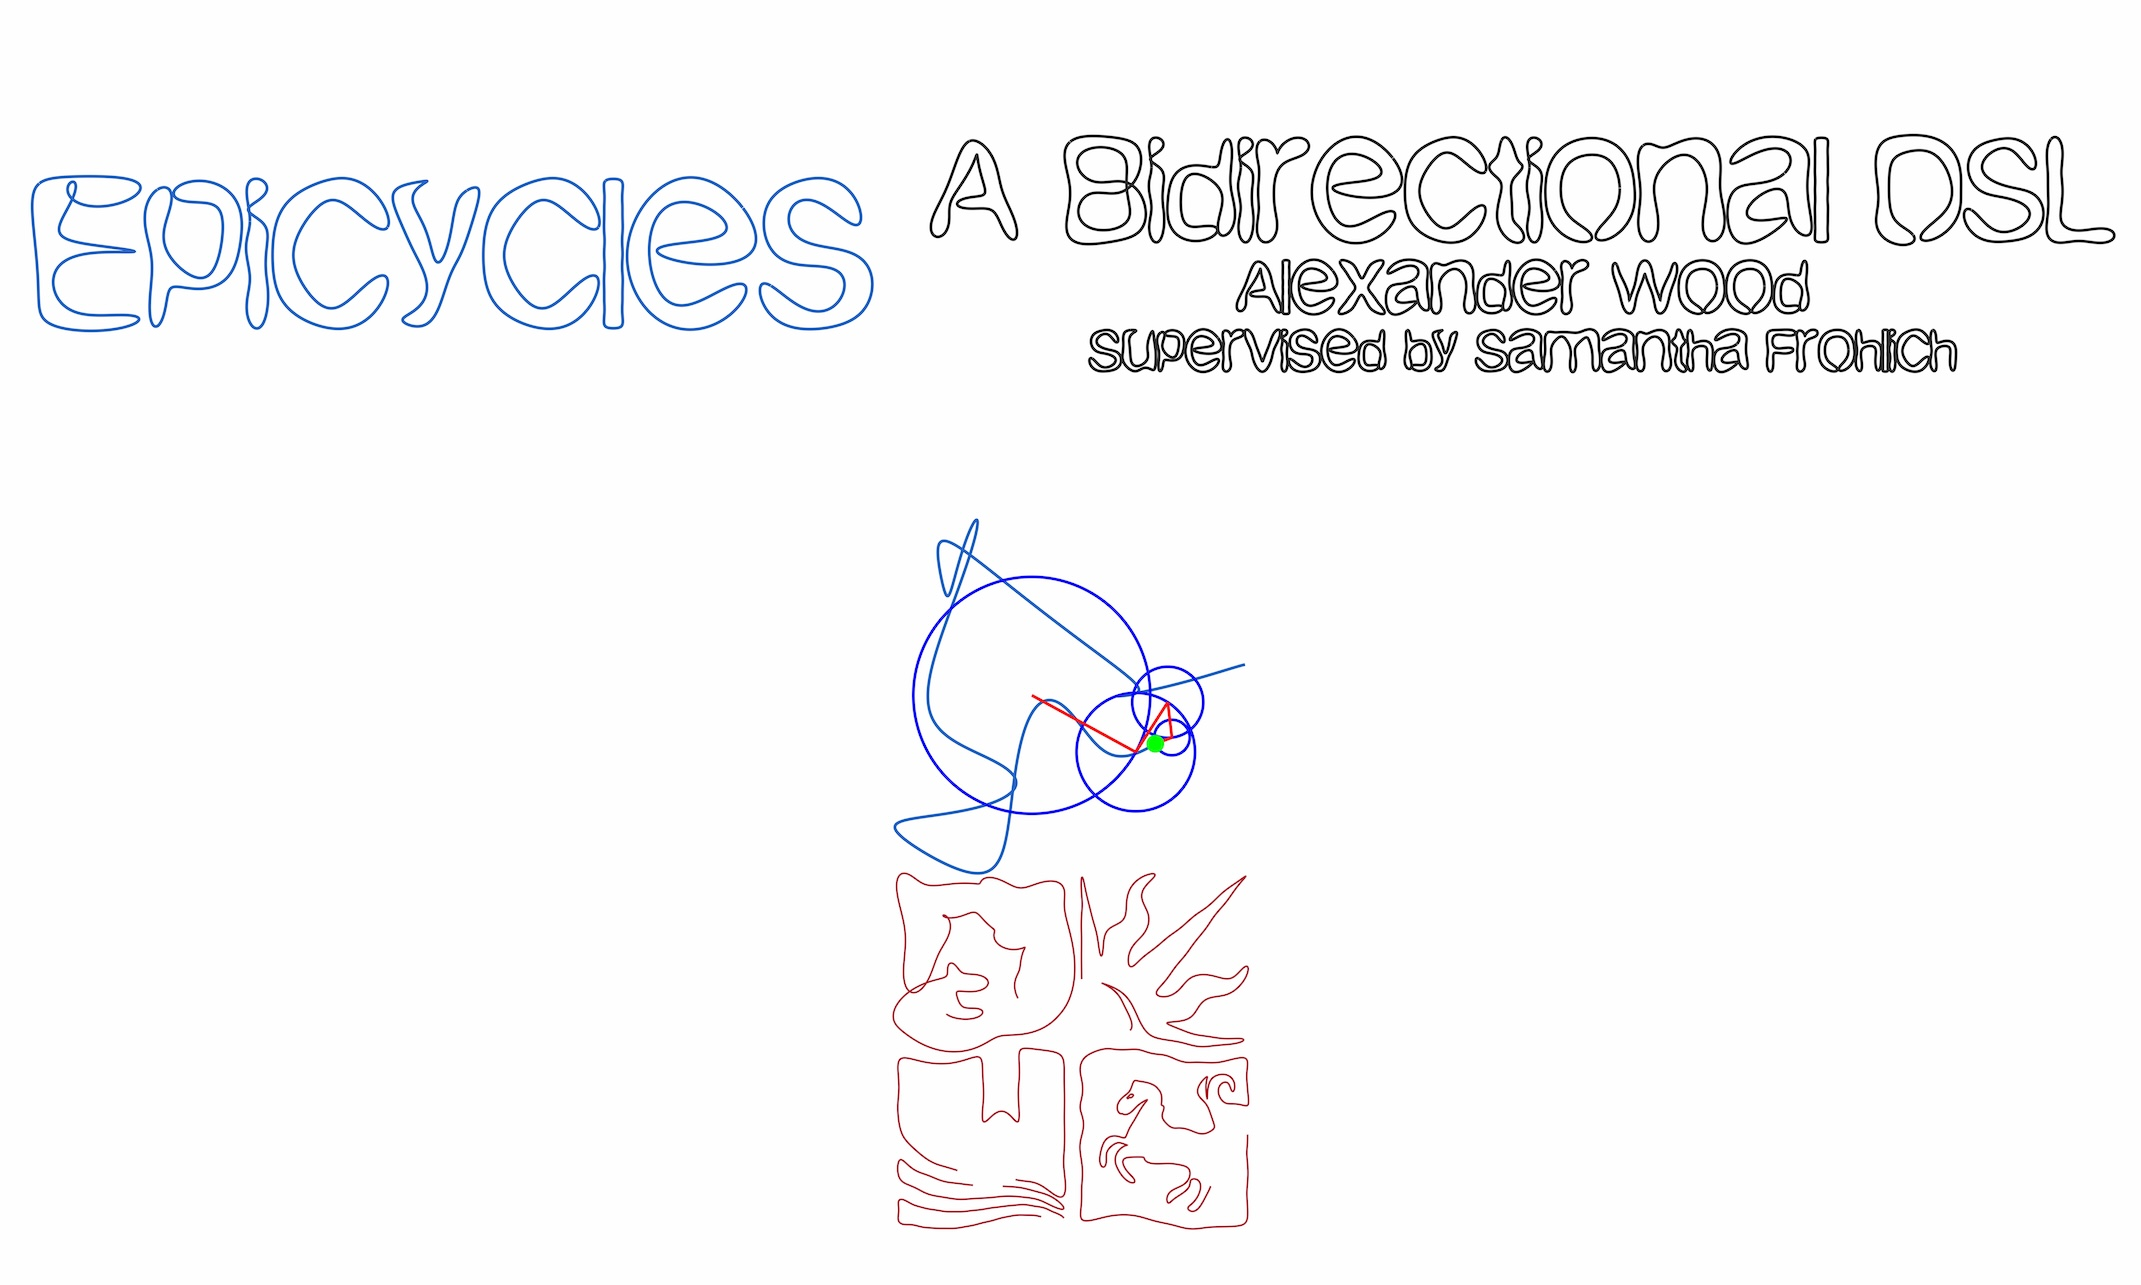
\includegraphics[width=0.8\textwidth]{images/simplified-poster.jpg}
	\caption{A simplified version of our Poster Day poster, generated with the DFT-based functionality of our DSL.}
	\label{fig:poster}
\end{figure*}


We add a DFT-based drawing tool to our UI, which allows users to draw a simple curve which is converted to a term in our DSL via the same method. This improves the creative coding potential of our system, as users can truly iterate in either direction -- they can draw a curve, then edit the generated program, or write a program, then edit the generated curve.

However, we should note that the epicycle-based abstraction is not without its flaws. The fundamental problem is that while the DFT can approximate any curve, it becomes very inefficient for certain types of curves, especially any sort of sharp corner. Drawing a square, for example, requires an infinite number of epicycles to be perfectly represented.
The Fourier-series representation remains powerful, and expressive in ways one might not initially consider. For instance, we are able to model straight line segments with two epicycles, by giving them inverse frequencies and the same radius. For a simple example, consider $\text{epicycle}(r, \omega, \phi) \oplus \text{epicycle}(r, -\omega, \phi)$. This represents the curve $c(t) = r \cdot e^{2\pi i (\omega t + \phi)} + r \cdot e^{-2\pi i (\omega t + \phi)}$ which simplifies:
\begin{align*}
	c(t) & = r \cdot e^{2\pi i \omega t + \phi} + r \cdot e^{-2\pi i \omega t + \phi} \\
	     & = r e^{i \phi} (e^{2\pi i \omega t} + e^{-2 \pi i \omega t})               \\
	     & = r e^{i \phi} (2 \cos(2\pi \omega t))                                     \\
	     & = 2 r \cos(2\pi \omega t) \cdot e^{i \phi}
\end{align*}

This essentially is a complex unit vector ($e^{i \phi}$) multiplied by a smoothly oscillating real component $2 r \cos(2\pi \omega t)$, and thus traces a straight line at angle $\phi$. Formally, this models a specific type of roulette known as a Tusi Couple.


Where the limitation does bite is in encoding efficiency for genuinely polygonal or text-like content: rendering text, for example, needs at least 6 epicycles per character for any kind of recognisable result, and around 10 to be considered a `good approximation' of real text. We demonstrate this in \cref{fig:fourier-cycles}.


Furthermore, editing the generated programs, while semantically correct (in most cases), does not necessarily translate to an intuitive user experience. Dragging an epicycle in a DFT-generated glyph curve, for example, usually has the effect of distorting the curve to the point of destroying its recognisability as a glyph, rather than producing an interesting transformation of the glyph, which the user might expect. We consider this primarily to be a limitation of the target domain -- the ability to approximate text is fragile, and as the primary focus of our DSL is geometric art, largely a byproduct of the Fourier Series representation. We note that future work could include improving the DFT-based functionality to attempt to mitigate this issue, for example by more intelligently utilising the straight line approximations, or adding extra constraints to the generated program to preserve recognisability, however this is outside the scope of this project.

\begin{figure*}
	\centering
	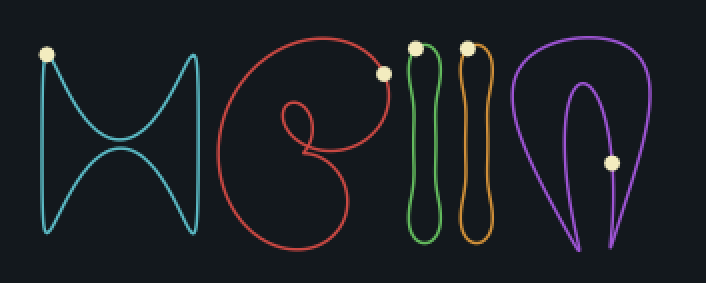
\includegraphics[width=0.4\textwidth]{images/hello-5-cycles.png}
	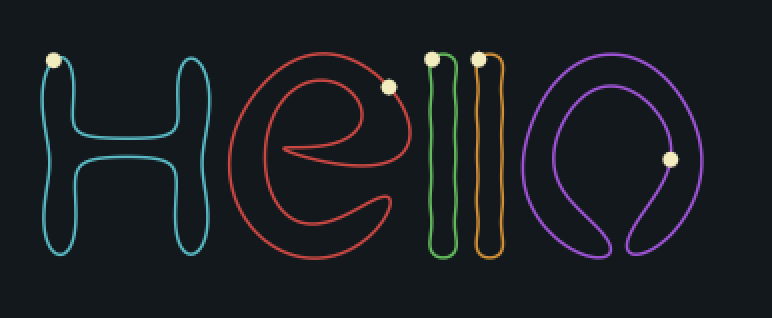
\includegraphics[width=0.4\textwidth]{images/hello-10-cycles.png}
	\caption{The text "Hello" interpolated with the Discrete Fourier Transform with 5 cycles per glyph (left) and 10 cycles per glyph (right).}
	\label{fig:fourier-cycles}
\end{figure*}

\subsection{Case Studies}

The primary focus with regards to creative coding for our DSL is to be able to express a variety of geometric curves. We evaluate this by presenting a number of case studies, showing different patterns and shapes that can be created with our DSL, alongside their source code.

\subsubsection{Gallery}

We demonstrate a few key examples of the types of images that can be produced with our DSL: \begin{itemize}
	\item \Cref{fig:straightline} shows the aforementioned straight line from two counter-spinning epicycles.
	\item \Cref{fig:deltoid} shows a \textit{Deltoid Curve}. This demonstrates that while sharp corners are difficult to represent, we are still able to approximate some polygonal-like curves
	\item In \cref{fig:harmonicDecay} we introduce the use of shared variables to our gallery, to create an effect of harmonic decay with epicycle radii.
	\item \Cref{fig:snowflake} shows a snowflake-like curve generated by exponentially decaying a shared radius parameter across 4 epicycles.
	\item \Cref{fig:dancer} demonstrates that our DSL is not limited to symmetric curves -- by sharing a parameter across the phase variable, we create an asymmetric pattern
	\item \Cref{fig:guilloche} shows a \textit{Guilloché Curve}\footnote{code loosely adapted from \url{https://mathworld.wolfram.com/GuillochePattern.html}}, a complex spirograph-like curve often used on banknotes.
\end{itemize}

\begin{figure*}
	\begin{minipage}[c]{0.4\textwidth}
		\centering
		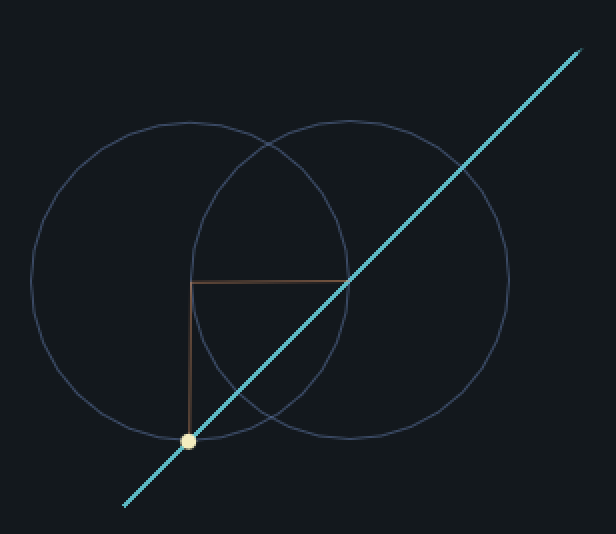
\includegraphics[width=\linewidth]{images/straight-line-demo.png}
	\end{minipage}\hfill
	\begin{minipage}[c]{0.5\textwidth}
		\begin{minted}{haskell}
straightLine =
  epicycle 80 3 0
    <> epicycle 80 (-3) (pi / 2)
	\end{minted}
	\end{minipage}
	\caption{A straight line at angle $\pi / 2$ formed of two epicycles, with construction enabled}
	\label{fig:straightline}
\end{figure*}


\begin{figure*}
	\begin{minipage}[c]{0.4\textwidth}
		\centering
		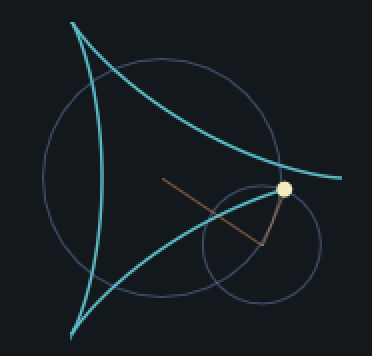
\includegraphics[width=\linewidth]{images/deltoid.png}
	\end{minipage}\hfill
	\begin{minipage}[c]{0.5\textwidth}
		\begin{minted}{haskell}
deltoid =
  epicycle 60 1 0
    <> epicycle 30 (-2) 0
	\end{minted}
	\end{minipage}
	\caption{A deltoid curve formed of two epicycles, with construction enabled}
	\label{fig:deltoid}
\end{figure*}

\begin{figure*}
	\begin{minipage}[c]{0.4\textwidth}
		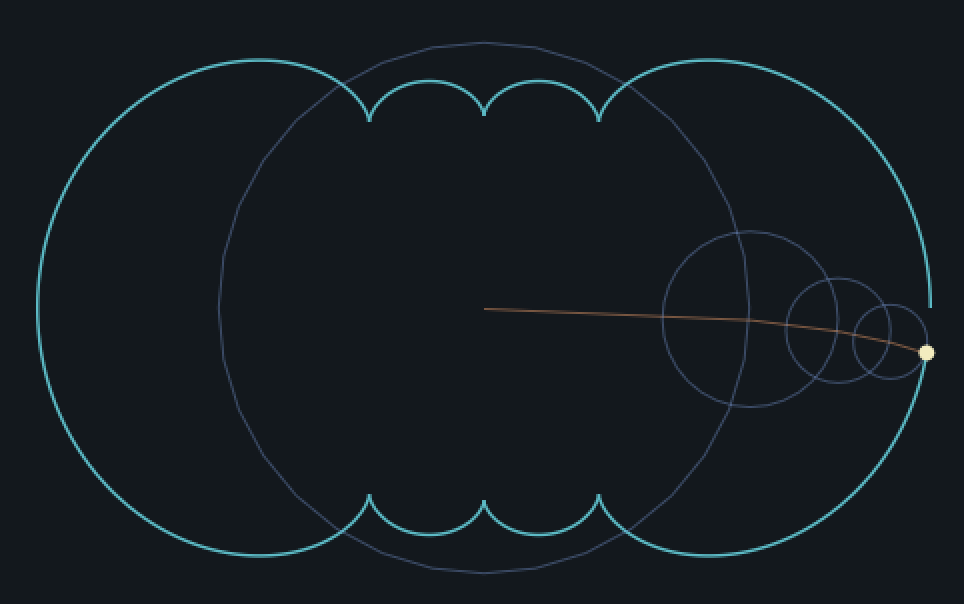
\includegraphics[width=\textwidth]{images/harmonic-decay.png}
	\end{minipage}\hfill
	\begin{minipage}[c]{0.5\textwidth}
		\begin{minted}{haskell}
curveSharedParameters = 
  let_ 60 $ \a ->
    epicycle a 1 0
      <> epicycle (a * recip 3) 3 0
      <> epicycle (a * recip 5) 5 0
      <> epicycle (a * recip 7) 7 0
	\end{minted}
	\end{minipage}
	\caption{A curve with a shared parameter used multiple times. The decreasing radii create a harmonic decay effect.}
	\label{fig:harmonicDecay}
\end{figure*}

\begin{figure*}
	\begin{minipage}[c]{0.4\textwidth}
		
\includegraphics[width=\textwidth]{images/snowflake.png}
	\end{minipage}\hfill
	\begin{minipage}[c]{0.5\textwidth}
		\begin{minted}{haskell}
snowflake = 
   let_ 60 $ \r ->
    epicycle r 1 0
        <> epicycle (r / 3) (-3) 0
        <> epicycle (r / 9) 9 0
        <> epicycle (r / 27) (-27) 0
	\end{minted}
	\end{minipage}
	\caption{A snowflake-like curve generated by exponentially decaying a shared radius parameter across 4 epicycles.}
	\label{fig:snowflake}
\end{figure*}

\begin{figure*}
	\begin{minipage}[c]{0.4\textwidth}
		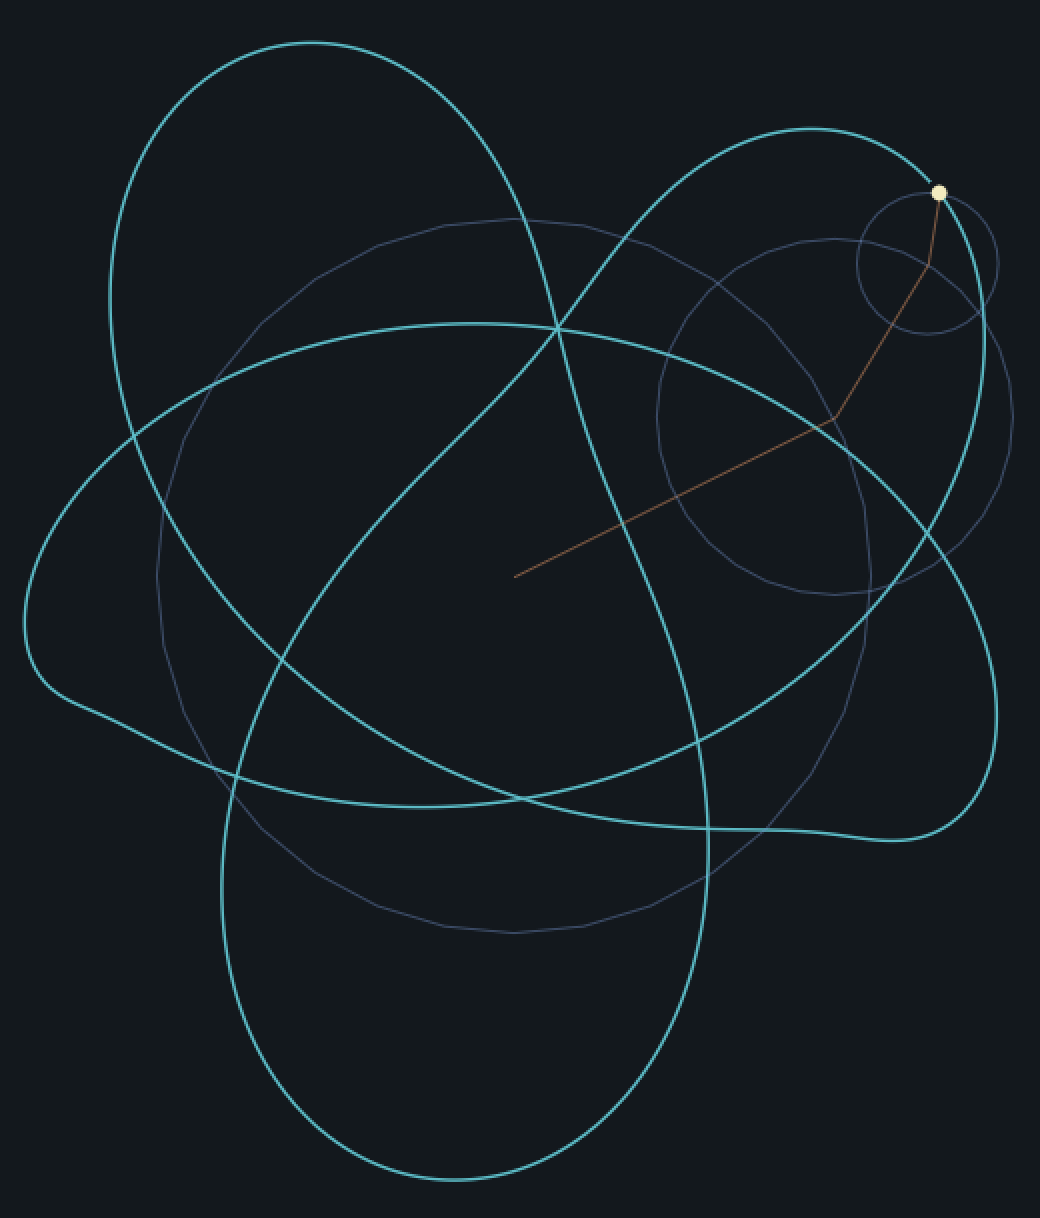
\includegraphics[width=\textwidth]{images/dancer.png}
	\end{minipage}\hfill
	\begin{minipage}[c]{0.5\textwidth}
		\begin{minted}{haskell}
asymmetric = 
  let_ 0.5 $ \p ->
    epicycle 60 3 p
      <> epicycle 30 (-2) (p * 2)
      <> epicycle 12 7 (p * 3)
	\end{minted}
	\end{minipage}
	\caption{An asymmetric curve generated by sharing a parameter across the phase variable.}
	\label{fig:dancer}
\end{figure*}

\begin{figure*}
	\begin{minipage}[c]{0.4\textwidth}
		
\includegraphics[width=\textwidth]{images/guilloche.png}
	\end{minipage}\hfill
	\begin{minipage}[c]{0.5\textwidth}
		\begin{minted}{haskell}
guilloche = 
 let_ 150 $ \r ->
    epicycle r 1 0
        <> epicycle (r * 0.15) (-4) 0
        <> epicycle (r * 0.12) 201 0
        <> epicycle (r * 0.12) (-196) 0
        <> epicycle (r * 0.04) 400 0
	\end{minted}
	\end{minipage}
	\caption{A Guilloché curve generated by sharing a radius parameter across 5 epicycles}
	\label{fig:guilloche}
\end{figure*}


\subsubsection{Parameter Editing}

We demonstrate the parameter editing capabilities with a short demonstration of how editing 1 frequency parameter can produce a visually varied response. We use the following demo program and use the GUI editing capabilities to vary the frequency of the second \verb|epicycle|
\begin{minted}{haskell}
demo =
  epicycle 50 1 0
    <> epicycle 50 2 0
\end{minted}

\Cref{fig:editing} shows the result of editing the frequency parameter to different values. We can see that a wide variety of curves can be produced by varying a single parameter, showing that our DSL's environment can be used effectively for artistic experimentation.


\begin{figure}
	\centering
	\begin{subfigure}{0.18\textwidth}
		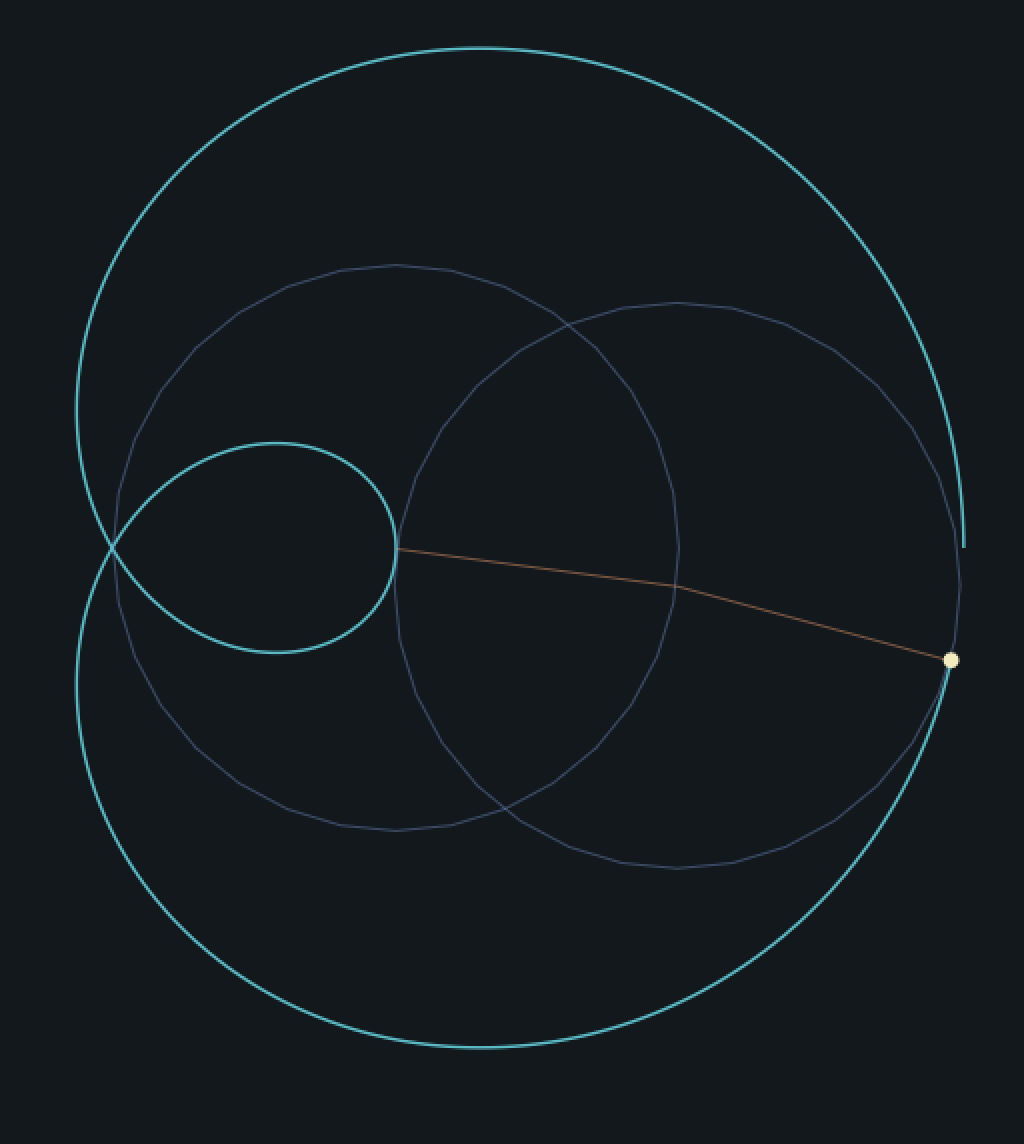
\includegraphics[width=\textwidth]{images/editing-f=2.png}
		\caption{$\omega_2=2$.}
		\label{fig:editing-first}
	\end{subfigure}
	\begin{subfigure}{0.18\textwidth}
		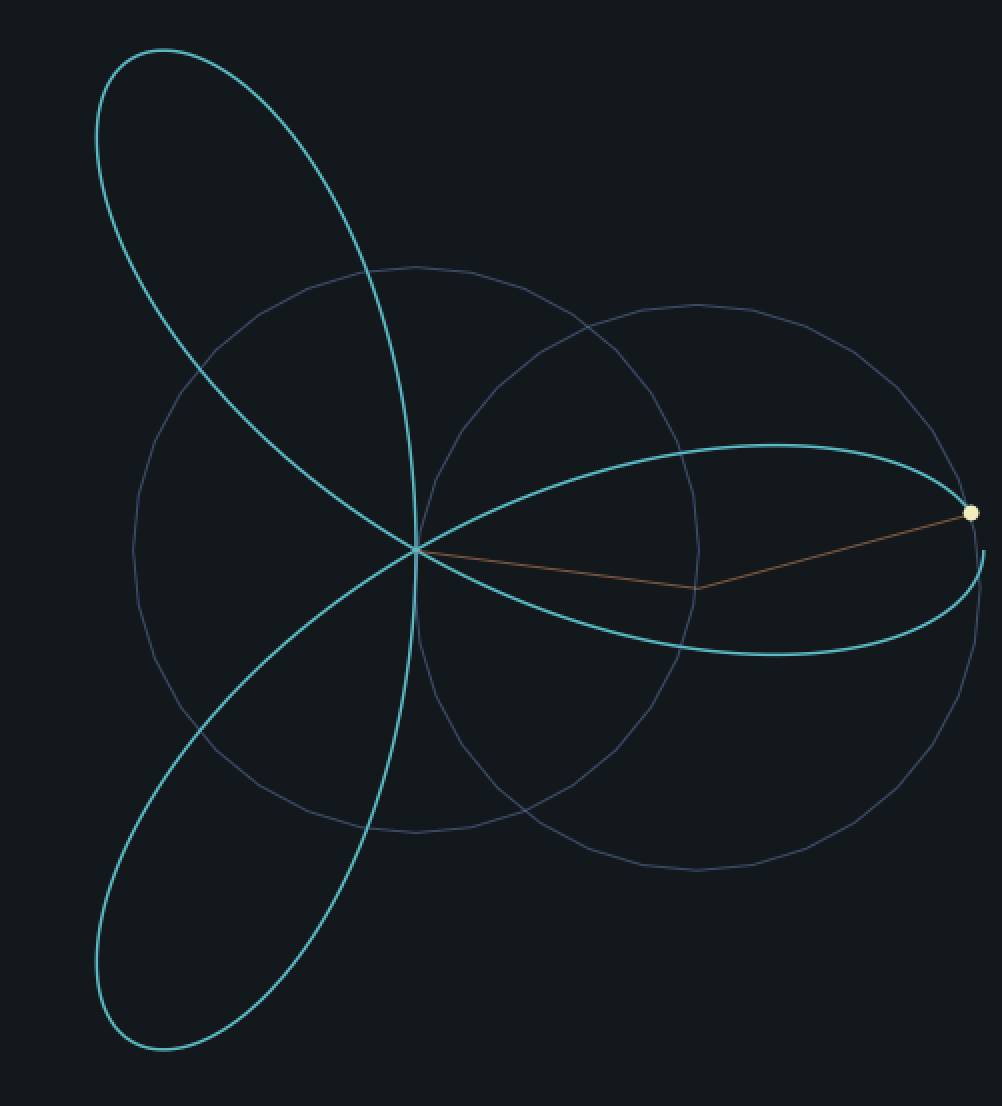
\includegraphics[width=\textwidth]{images/editing-f=-2.png}
		\caption{$\omega_2=-2$.}
		\label{fig:editing-second}
	\end{subfigure}
	\begin{subfigure}{0.18\textwidth}
		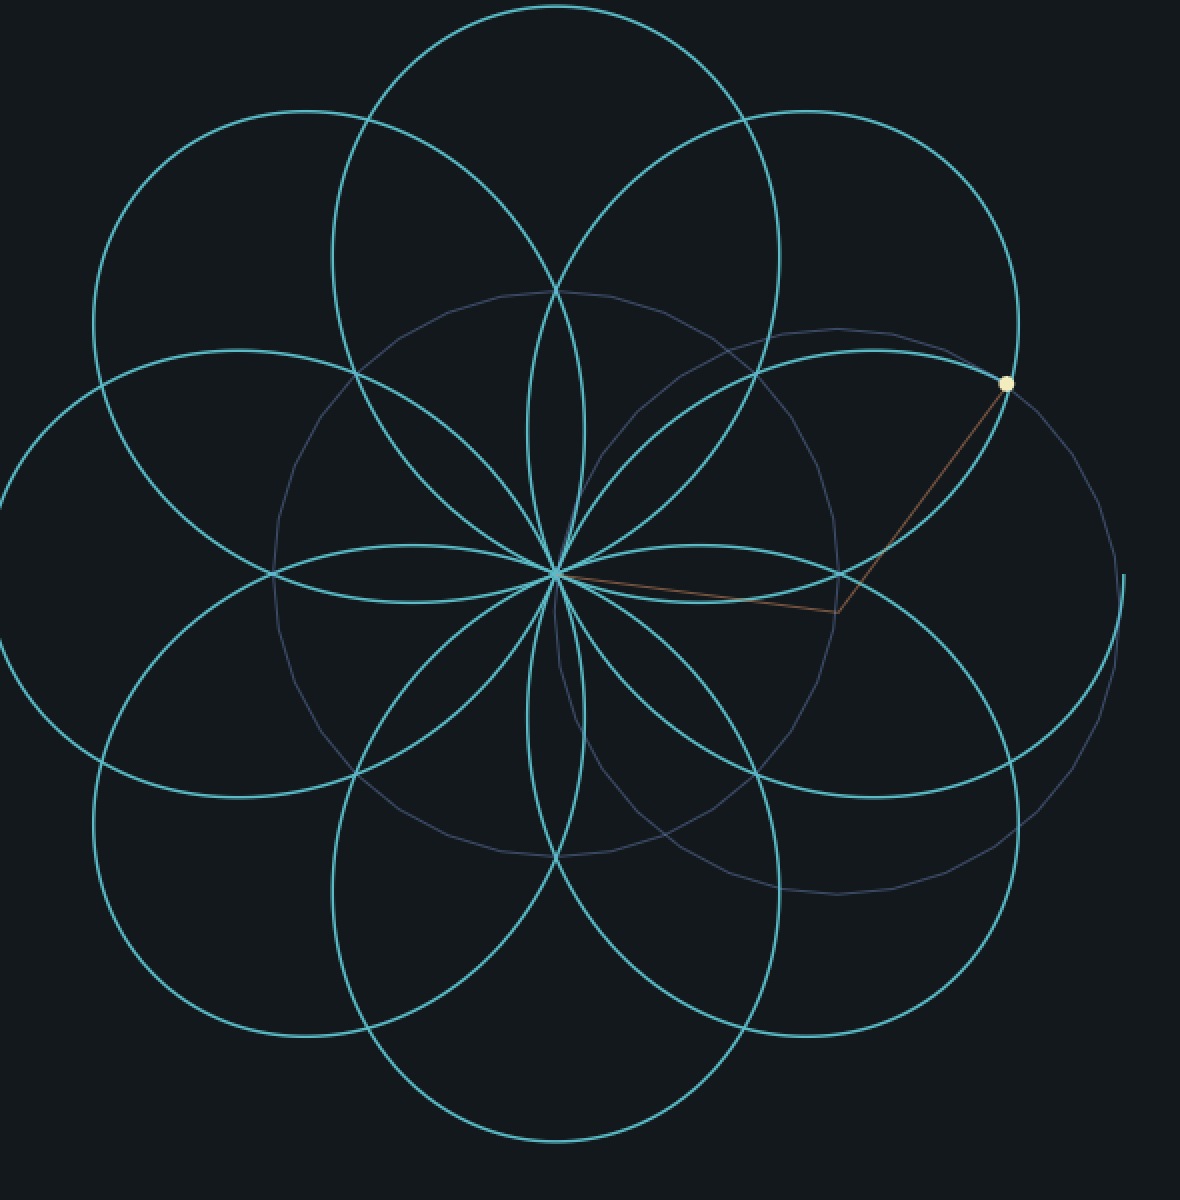
\includegraphics[width=\textwidth]{images/editing-f=-7.png}
		\caption{$\omega_2=-7$.}
		\label{fig:editing-third}
	\end{subfigure}
	\begin{subfigure}{0.18\textwidth}
		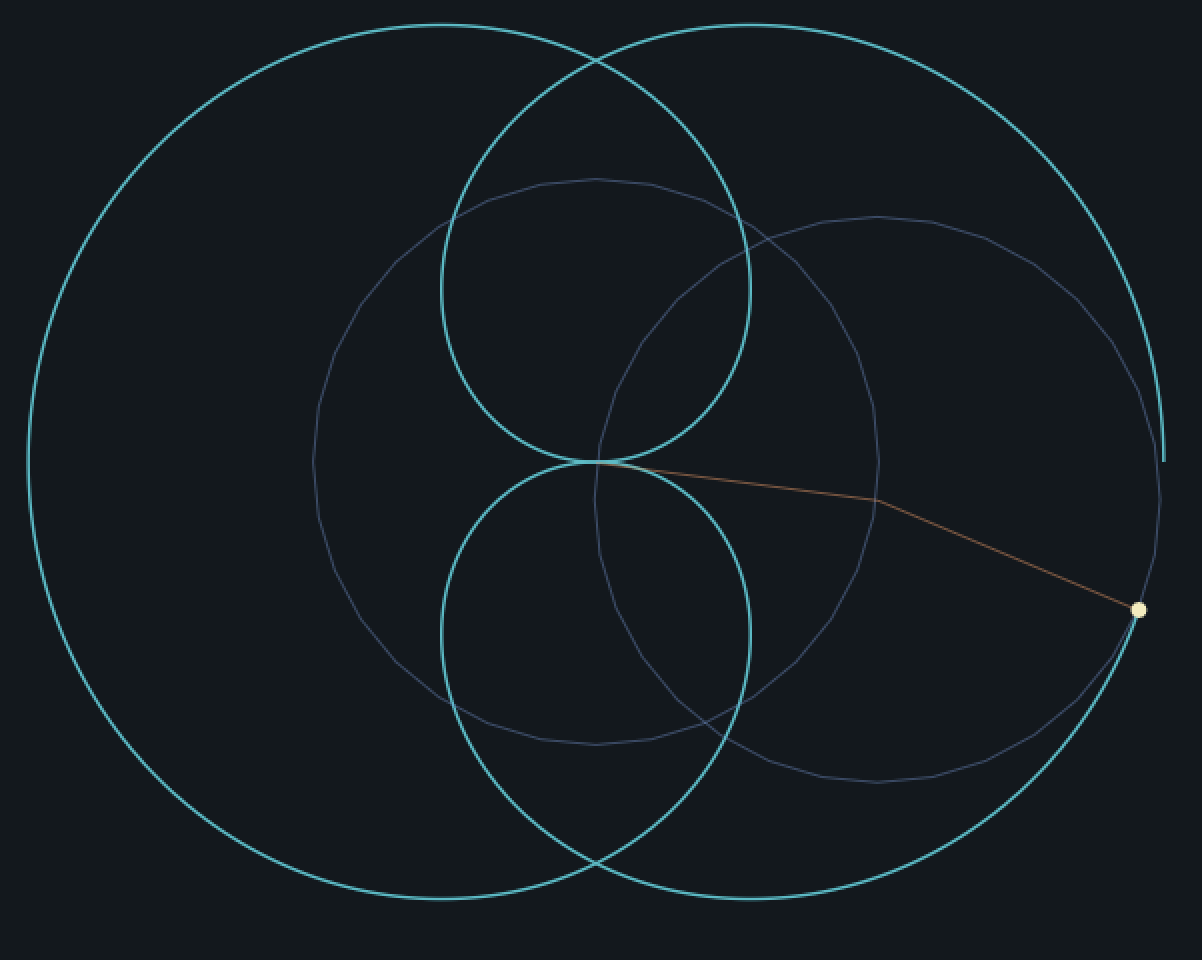
\includegraphics[width=\textwidth]{images/editing-f=3.png}
		\caption{$\omega_2=3$.}
		\label{fig:editing-fourth}
	\end{subfigure}
	\begin{subfigure}{0.18\textwidth}
		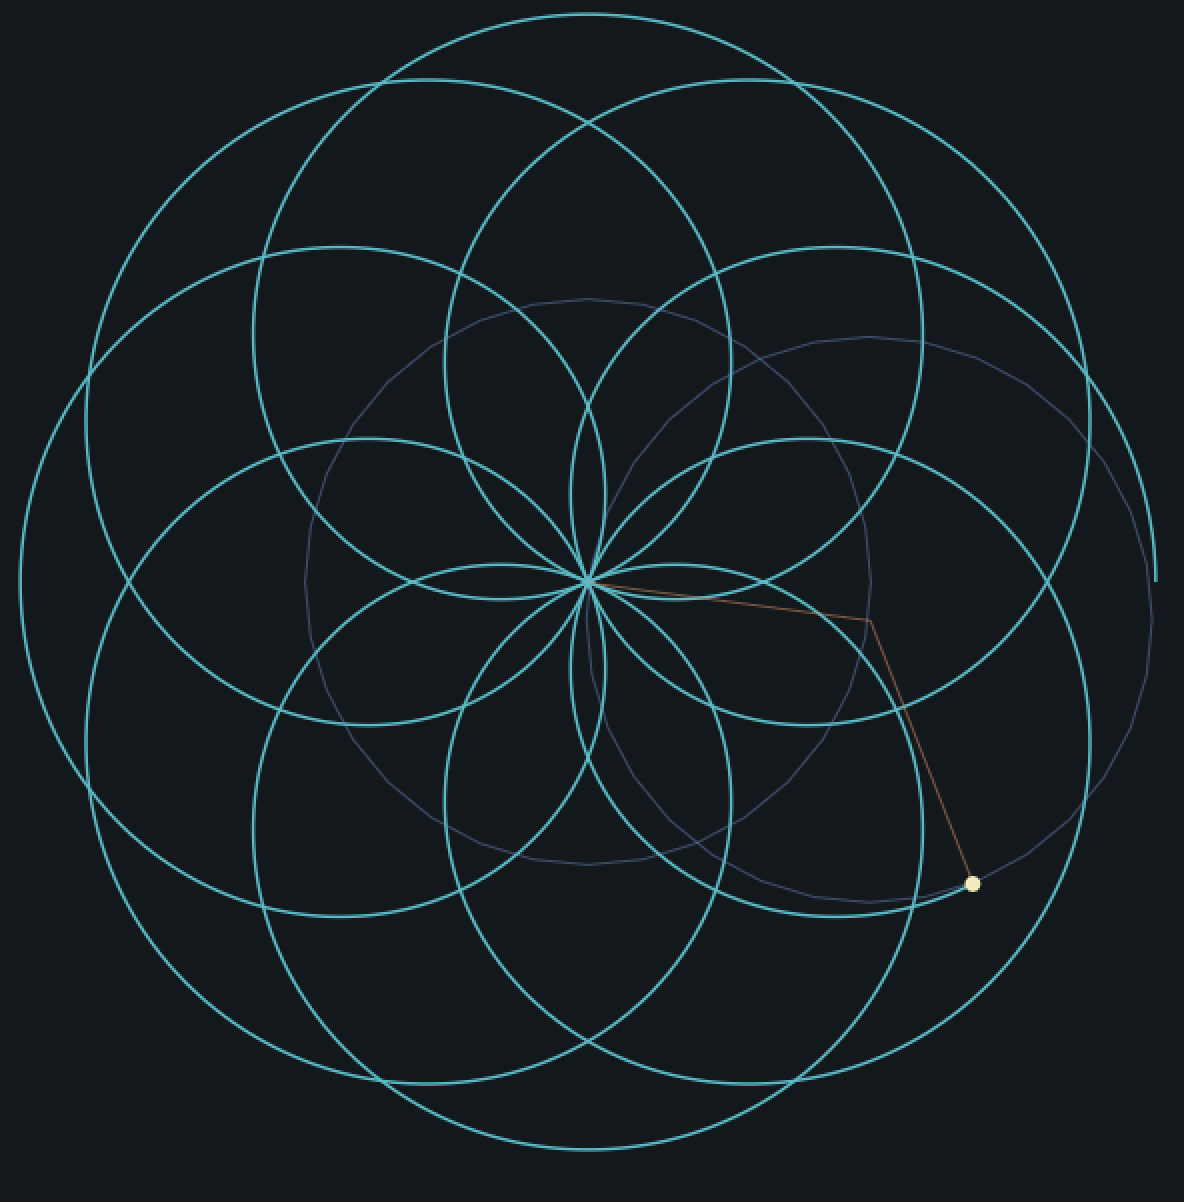
\includegraphics[width=\textwidth]{images/editing-f=9.png}
		\caption{$\omega_2=9$.}
		\label{fig:editing-fifth}
	\end{subfigure}
	\caption{Editing the frequency parameter $\omega_2$ of an epicycle produces a variety of different curves.}
	\label{fig:editing}
\end{figure}

\section{Direct Manipulation and User Experience}

Some of the biggest pitfalls of our User Experience come as a consequence of our choice to use an Embedded DSL. \Cref{chap:context} discussed live coding systems such as \textit{TidalCycles}, which we took a level of inspiration from, particularly the tight feedback loop that the live coding environment provided. Our system, however is slightly less fluid. The GUI does not provide a text editor for the source code due to the technical complexities of adding one. As our DSL is embedded in Haskell, parsing and evaluating the code relies on the entire GHC compiler and toolchain. Consequently, the curve programs must be within a larger Haskell file, which must be separately compiled and run, and then recompiled and re-ran upon edits.

There is scope for improvement here: \textit{TidalCycles}, for example, decouples the source code and evaluation into two different processes -- code can be written in any text editor, and is then `serialised' to an external daemon which interprets it. We initially considered this architecture, but concluded it would require significant engineering work that would detract from the core focus of the project: the design and formalisation of the DSL and its semantics. Novel solutions such as building a custom Language Server Protocol (LSP) implementation\footnote{\url{https://lambein.xyz/paw-live2023/}} to connect the output and text editor more directly are also worthy of future consideration. However, we acknowledge that the current separation is a limitation of our system.

Furthermore, the deep embedding causes our system to suffer from a lack of lexical round-tripping. Our UI contains a code panel showing the source of the rendered curves, however this is strictly an approximation generated by pretty-printing the AST, and is not the verbatim source code (edited or otherwise). Certain elements of the source code such as binder names cannot be reified at all due to the fundamental limitation of embedding, and so we are forced to assign variables generated names. Additional properties such as white space, comments, etc are also discarded.

These two factors combine to make a full bidirectional round-trip difficult -- an `Export Code' button, for example, would suffer from a number of implementation challenges: the DSL cannot be printed `as-is', as some extra Haskell preamble is needed -- the system would need to be very sensitive to avoid overwriting this. Heavily formatted code would also be overwritten by the system's standardised output, disrupting the programmer's workflow.

This motivates moving to a bespoke DSL with its own parser and editor in future work, which would address these limitations. While we lose the benefits of embedding such as being able to reuse Haskell's type system, the engineering work in reimplementing the subset of features we use would not be prohibitive given more time.

We consider this an acceptable limitation due to our language being relatively minimal, so manually synchronising the updated code to the editor is generally feasible and not overly cumbersome. A simpler `copy snippet' button would also provide a suitable compromise, particularly for more complex curve definitions such as the result of a hand-drawn trace.



\section{Metrics} \label{sec:metrics}
While the formal properties established in \Cref{sec:properties} provide theoretical guarantees, we run quantitative metrics on the semantics to measure the practical boundaries and severity of their theoretical limitations. Specifically, we evaluate:
\begin{itemize}
	\item \textbf{Intent Leakage and Reversibility}: How effectively a sequence of edits can be `reversed', and the magnitude of `collateral damage' caused to surrounding epicycles
	\item \textbf{AST Growth Bounds}: the increase in the size of the AST after the update, in terms of total node count.
	\item \textbf{PutPut failures}: the rate of PutPut failures, including both asymmetric failures and disagreements, across a number of sequential edits.
\end{itemize}

\paragraph{Scene Catalogue.}
We design a small catalogue of test scenes designed to simulate the different strengths and weaknesses of the different semantics. These include a few simple curves as baselines, curves with intense use of shared parameters, and simulating edge cases such as the counterexample discussed in \cref{par:putput-sns}.

We measure all these metrics over a number of varied \textit{scenarios}, which provide different types of edits. Some scenarios are designed to simulate real user interaction, some are designed for stress testing, and some replicate edge cases that the UI never permits:
\begin{itemize}
	\item \textbf{BigJump}: a large delta between the initial and target value
	\item \textbf{RandomWalk}: a series of random deltas applied sequentially, simulating a user experimenting
	\item \textbf{Drag}: a series of monotonic deltas applied sequentially, simulating a user dragging an epicycle in one direction
	\item \textbf{Oscillate}: a series of alternating positive and negative deltas applied sequentially
	\item \textbf{SiblingChain}: for each adjacent epicycle pair $(i, i+1)$, apply a delta to $i$ then $i+1$ then $i$ then $i+1$, etc.
\end{itemize}

\subsection{Quantifying the AST Growth} \label{par:ast-growth}
We formalised in \Cref{theorem:fixedpoint} that the FuseDM-based semantics cause the AST to expand until all shared variables are `shielded' by synthesised nodes.
We investigate whether this expansion renders the resulting source code unreadable or computationally bloated.
We find that our theorem holds in practice -- the standard deviation of AST growth over 20-25 series of random edits is exactly zero. This proves that over time, the embedding operator does cause the AST to converge to a final fixed point. Furthermore, we observe the size of the AST growth to be manageable: the maximum growth across all scenarios and scenes is approximately $1.4 \times$, going from an initial curve of 24 nodes, to a final of 34 nodes. Some curves exhibited zero growth (if they have no shared variables), and the average growth overall (excluding cases of zero growth) is approximately $1.3 \times$, which we argue is an acceptable and manageable increase that would not impact the readability of the final code.

\begin{table}[ht]
	\centering
	\begin{tabular}{lcccccc}
		\hline
		\textbf{Scene} & \textbf{Initial} & \textbf{Final Min} & \textbf{Final Max} & \textbf{Final Std} & \textbf{Growth} & \textbf{Runs} \\ \hline
		AddAlias       & 8                & 10                 & 10                 & 0.000              & 1.250x          & 20            \\
		Ambiguous      & 33               & 33                 & 33                 & 0.000              & 1.000x          & 25            \\
		DeepShared     & 34               & 44                 & 44                 & 0.000              & 1.294x          & 25            \\
		DualRecip      & 12               & 12                 & 12                 & 0.000              & 1.000x          & 20            \\
		LeftBias       & 19               & 23                 & 23                 & 0.000              & 1.211x          & 25            \\
		MulAlias       & 8                & 8                  & 8                  & 0.000              & 1.000x          & 20            \\
		NestedLet      & 20               & 28                 & 28                 & 0.000              & 1.400x          & 25            \\
		Shared         & 24               & 34                 & 34                 & 0.000              & 1.417x          & 25            \\
		Simple         & 14               & 14                 & 14                 & 0.000              & 1.000x          & 25            \\
		SquareAlias    & 8                & 10                 & 10                 & 0.000              & 1.250x          & 20            \\ \hline
	\end{tabular}
	\caption{AST Size Growth under FuseDM semantics. The zero standard deviation across runs confirms convergence to a structural fixed point.}
	\label{tab:ast-growth}
\end{table}

\subsection{Intent Leakage and Reversibility}
In contrast, we measure how the semantics handle a `net-zero' user interaction with the \textbf{Oscillate} scenario (as the edits return to the original state). In a perfectly reversible system, this should leave both the AST and the visual output entirely unchanged. We also measure `intent leakage', which can be viewed as quantifying the magnitude of a violation of the PutGet law when considering the entire curve as the view. In other words, an edit `leaks` if it causes `collateral damage' to other epicycles which were not directly interacted with.

Our metrics show that this property comes at odds with semantic purity: the SnS-based strategies (both Heuristic and Naive) demonstrate 100\% structural reversibility, returning the AST to its exact initial size and shape. This is to be expected, as the semantics cannot structurally change the AST. However, this comes at the cost of silently corrupting the semantic state -- over 50 runs on scenes with shared variables, the Naive update `leaked' an average of 1080 unintended changes to sibling epicycles. The Heuristic strategy's cost-ranking mitigates this (averaging 330 leaked changes), but does not (and cannot) eliminate it.

Conversely, the FuseDM semantics' AST rewriting causes it to exhibit a mere 40\% structural reversibility rate -- i.e. in 60\% of cases, some edits cause the AST to be permanently altered due to the literal shielding. However, its mean intent leakage is exactly 0.0. This demonstrates that while the SnS approach maintains an illusion of an untouched source file, it more subtly disrupts the (potential) user intention. In contrast, FuseDM sacrifices the original AST shape, potentially adding some user friction, to guarantee that unedited epicycles remain unchanged -- potentially better matching the user's intent.


\begin{table}[ht]
	\centering
	\begin{tabular}{lccccc}
		\hline
		\textbf{Strategy} & \textbf{Returned \%} & \textbf{Mean Leak} & \textbf{Median} & \textbf{Max} & \textbf{Runs} \\ \hline
		Heuristic         & 100.0                & 330.0              & 0.0             & 1200         & 50            \\
		Naive             & 100.0                & 1080.0             & 0.0             & 6000         & 50            \\
		FuseDM            & 40.0                 & 0.0                & 0.0             & 0            & 50            \\ \hline
	\end{tabular}
	\caption{Intent leakage and structural reversibility when oscillating on shared scenes.}
	\label{tab:reversibility}
\end{table}

\subsection{PutPut Failure}
Finally, we evaluate the rate of PutPut failures across a large amount of edits, examining two types of PutPut failure: `asymmetric failures', when one path succeeds but the other fails (the stability failure mentioned in \cref{par:putput-sns}), and `disagreements' when both paths succeed but produce different final states. We observe that once again, the FuseDM-based semantics always satisfy PutPut, whereas the Sketch-n-Sketch-based semantics occasionally fail, at an overall rate of approximately 5.79\%. This primarily manifests as end-state disagreements, alongside a smaller 0.61\% rate of asymmetric failures where the solver forces itself down invalid mathematical branches.
The most significant example of PutPut failure on the SnS-based semantics was with the following program, which failed on almost 70\% of edits:
\begin{minted}{haskell}
curve = 
  let_ 10 $ \r ->
    epicycle (r * r) 1 0
\end{minted}

\begin{table}[ht]
	\centering
	\begin{tabular}{lccccc}
		\hline
		\textbf{Strategy} & \textbf{Intermediate OK \%} & \textbf{Direct OK \%} & \textbf{Asymm \%} & \textbf{End Dis \%} & \textbf{Combined \%} \\ \hline
		SnS               & 99.39                       & 100.00                & 0.61              & 5.79                & 5.79                 \\
		FuseDM            & 100.00                      & 100.00                & 0.00              & 0.00                & 0.00                 \\ \hline
	\end{tabular}
	\caption{PutPut violation rates across 984 tests.}
	\label{tab:putput}
\end{table}

This exposes the biggest failure of our SnS-based semantics thus far: the locality of the semantics. Just as our initial lens-based prototype failed, this fails so frequently because the semantics are unaware of the structure of the expression. When updating to a new $v'$, the \textsc{U-Mul} rules try to update each $r$ individually to some new $r'$ such that $r' * r' = v'$, blind to the fact that both occurrences refer to the same variable, which produces invalid updates that fail PutGet \textit{and} PutPut in almost all cases. The true solution, $r = \sqrt{v'}$ is never in the candidate set using our rules. This is a fundamental limitation of these semantics, not the heuristics -- the valid solution will almost never be in the candidate set. We must either filter out the bad updates, which makes the drag do nothing, or allow them despite being malformed, which causes an unpredictable user experience and `jitters' in the UI -- both solutions are unsatisfactory. Sketch-n-Sketch does not attempt to solve issues like this itself, instead delegating the work to an external Computer Algebra System\cite{hempel_sketch-n-sketch_2019}. We do not do such a thing, and instead accept this as a limitation which motivates the use of the delta-based semantics instead. We note that this issue could be alleviated in many cases by extending the candidate set to attempt some more complex updates -- for example, we might introduce some new rule which tries the solution $\sqrt{v'}$ if the expression $e_1 \times e_2$ happens to also evaluate to $e_1 \times e_1$.
\begin{mathpar}
	\inferrule*[right=U-Mul-Sqrt]
	{\sigma \vdash e_1 \times e_2 : \eta \Downarrow v_1
		\\ \sigma \vdash e_1 \times e_1 : \eta \Downarrow v_2
		\\ v_1 = v_2
		\\  \sigma \vdash e_1 : \eta \Uparrow \sqrt{v'}\rightsquigarrow (\sigma_1, e_1') }
	{ \sigma \vdash e_1 \times e_2 : \eta \Uparrow v' \rightsquigarrow (\sigma_1, e_1' \times e_2) }
\end{mathpar}
This approach does not generalise though -- each new rule increases the size of our candidate set exponentially, and just as with our failed prototype, we tend towards reinventing a Computer Algebra System. The possibility of failure is a fundamental limitation of this style of semantics.


\section{Automated Testing}

We also construct a small suite of \textit{property tests}\cite{claessen_quickcheck_2000} using the \textit{Hedgehog} Haskell library,  to further verify our theoretical claims. For example, we write some tests about exactly how many candidates the SnS update returns for a given AST and edit.
The majority of these tests are properties we have already formally proven, but these tests serve as an extra sanity check, catching engineering bugs in our implementation

\section{Summary}

We conclude that for our particular domain, and bidirectional programming as a whole, the delta-based semantics are superior to the Sketch-n-Sketch ones, due to its more lawful behaviour, which makes it easier to reason about, and more intuitive for the user.
We consider the many extra cases required to prove basic properties like GetPut and PutGet on the SnS semantics, due to the numerous edge cases, which, in some situations, manifest as an unacceptably high failure rate of editing.





% \begin{figure*}
% 	\centering
% 	\begin{tabular}{ |c|c|c|c| }
% 		\hline
% 		                   & \textbf{Asymmetric Failures} & \textbf{Disagreements } & \textbf{Combined} \\
% 		\hline
% 		\textbf{FuseDM}    & 0.00\%                       & 0.00\%                  & 0.00\%            \\
% 		\hline
% 		\textbf{Heuristic} & 0.54\%                       & 0.54\%                  & 0.54\%            \\
% 		\hline
% 		\textbf{Naive}     & 0.54\%                       & 0.54\%                  & 0.54\%            \\
% 		\hline
% 	\end{tabular}
% 	\caption{PutPut failure rates for the three semantics aggregated across approximately 1100 edit oeprations.}
% 	\label{fig:putput}
% \end{figure*}

% {\bf A topic-specific chapter}
% \vspace{1cm}

% \noindent
% This chapter is intended to evaluate what you did.  The content is highly
% topic-specific, but for many projects will have flavours of the following:

% \begin{enumerate}
% 	\item functional  testing, including analysis and explanation of failure
% 	      cases,
% 	\item behavioural testing, often including analysis of any results that
% 	      draw some form of conclusion wrt. the aims and objectives,
% 	      and
% 	\item evaluation of options and decisions within the project, and/or a
% 	      comparison with alternatives.
% \end{enumerate}

% \noindent
% This chapter often acts to differentiate project quality: even if the work
% completed is of a high technical quality, critical yet objective evaluation
% and comparison of the outcomes is crucial.  In essence, the reader wants to
% learn something, so the worst examples amount to simple statements of fact
% (e.g., ``graph X shows the result is Y''); the best examples are analytical
% and exploratory (e.g., ``graph X shows the result is Y, which means Z; this
% contradicts [1], which may be because I use a different assumption'').  As
% such, both positive {\em and} negative outcomes are valid {\em if} presented
% in a suitable manner.

% -----------------------------------------------------------------------------

\chapter{Conclusion}
\label{chap:conclusion}

Our core thesis is that a well-chosen domain restriction makes the View-Update problem tractable. We demonstrate this by designing and implementing a DSL and UI for bidirectional creative coding geometric art by composing epicycles. We show that our DSL is expressive enough to model a variety of visually interesting curves, and that our UI allows intuitive and unambiguous direct manipulation of these curves.

On a technical level, we use modern, advanced techniques to implement our embedded DSL in Haskell, with a high-level HOAS interface which `compiles' to a lower level FOAS AST, allowing for a readable frontend language without losing introspective power. We use industry-standard design patterns such as \textit{Trees that Grow} to encode the invariants of our DSL into Haskell's type system, making invalid states unrepresentable -- our implementation contains zero partial functions or unsafe pattern matches (excluding tests).

We implement two different semantics for bidirectional evaluation of our DSL, one based on the non-deterministic Sketch-n-Sketch system, and another based on the AST-rewriting FuseDM system, satisfying our first two aims in our introduction.

We adjust these semantics to work with our language, and prove common correctness properties such as PutGet and GetPut on them with the Lean theorem prover. We also evaluate the two semantics quantitatively, running them on a large test suite and evaluating their success and failure rates in the context of creative coding. We discuss the flaws of each system in depth both theoretically and for practical usage, satisfying our third aim.

Finally, we evaluate the expressivity of our DSL, exploring the creative potential of our domain restriction. We demonstrate that we can model a myriad of curves, and can use the Discrete Fourier Transform to approximate things like text, images, and user-drawn curves. We identify the weaknesses of the domain, such as inefficient or unintuitive encodings of more complex curves, and visual fragility when editing due to a lack of constraints.

A key outcome of this evaluation is the identification of a fundamental trade-off in bidirectional systems: the choice between \textit{structural reversibility} and \textit{intent preservation}. While the Sketch-n-Sketch approach maintains the original source code's shape, it produces updates which can `corrupt' other parts of the program, causing the original intent to degrade. In contrast, the delta-based approach prioritises matching the user's intent as closely as possible, at the cost of making structural changes to the program. We argue that in a creative context, where the visual output is the primary object of concern, the penalty of this `literal shielding' is a small price to pay for the more intuitive semantics.

The future work identified in this project is clear. The simple interaction model of our system does not allow the power of the delta-based semantics to fully show themselves: although we support a more complex family of deltas, there is no way to trigger these from the UI. This was mainly due to designing the interaction model around the simpler Sketch-n-Sketch based semantics, which may struggle with more complex edits.
Moving forward, we would focus on the delta-based semantics and exploring how to expand the system and use it more effectively. For example, we would investigate addressing the fragility of the text approximation by exploring ways to add constraints to updates. This could tie in with our observation that we under-utilise the delta semantics; for example, we could explore ways of grouping updates, where an edit to one part of a curve propagates a synchronised delta to a cluster of related epicycles, preserving the structure while still allowing updates.
We also noted that while the PutGet law is valuable from a theory perspective, sometimes the user does \textit{want} to violate it when they have defined a shared variable -- a useful future direction would be to explore ways of allowing the user to explicitly choose when to violate PutGet in a controlled way that still behaves predictably. One option would be taking the opposite approach to Sketch-n-Sketch: rather than having a \verb|!| operator to `lock' values, we have an operator to `unlock' them, allowing them to be edited in ways that violate PutGet, but only when the user explicitly opts in to this behaviour. Any additions in this direction should carefully evaluate the amount of work they force the user to do -- our system succeeds in part because it `just works', and adding more and more extra tools to the kit could cause more friction when creative coding.

A promising future avenue would be to take the lessons we have learned from this project to a new, less restricted creative domain. For example, we may revisit our failed initial prototype with a delta based approach to investigate how far we can take it with a more thoughtful design. Informal user feedback of Epicycles also identified some more practical examples of where a system like this may be useful, namely drawing TikZ diagrams in \LaTeX -- a visual domain with a reputation for poor feedback loops and no support for direct manipulation.

In conclusion, this project demonstrates that by carefully restricting the programming and artistic domains, we can bridge the `abstraction gap' between code and visual output in such a way that allows for tractable solutions to the View-Update problem, without sacrificing expressivity. While general-purpose bidirectional programming remains an open challenge, the success of our DSL suggests that domain-specific solutions provide a practical, lawful, and expressive path for the next generation of creative tools.

% \noindent
% The concluding chapter of a dissertation is often underutilised because it
% is too often left too close to the deadline: it is important to allocate
% enough attention to it.  Ideally, the chapter will consist of three parts:

% \begin{enumerate}
% 	\item (Re)summarise the main contributions and achievements, in essence
% 	      summing up the content.
% 	\item Clearly state the current project status (e.g., ``X is working, Y
% 	      is not'') and evaluate what has been achieved with respect to the
% 	      initial aims and objectives (e.g., ``I completed aim X outlined
% 	      previously, the evidence for this is within Chapter Y'').  There
% 	      is no problem including aims which were not completed, but it is
% 	      important to evaluate and/or justify why this is the case.
% 	\item Outline any open problems or future plans.  Rather than treat this
% 	      only as an exercise in what you {\em could} have done given more
% 	      time, try to focus on any unexplored options or interesting outcomes
% 	      (e.g., ``my experiment for X gave counter-intuitive results, this
% 	      could be because Y and would form an interesting area for further
% 	      study'' or ``users found feature Z of my software difficult to use,
% 	      which is obvious in hindsight but not during at design stage; to
% 	      resolve this, I could clearly apply the technique of Smith [7]'').
% \end{enumerate}

% =============================================================================

% Finally, after the main matter, the back matter is specified.  This is
% typically populated with just the bibliography.  LaTeX deals with these
% in one of two ways, namely
%
% - inline, which roughly means the author specifies entries using the 
%   \bibitem macro and typesets them manually, or
% - using BiBTeX, which means entries are contained in a separate file
%   (which is essentially a databased) then inported; this is the 
%   approach used below, with the databased being dissertation.bib.
%
% Either way, the each entry has a key (or identifier) which can be used
% in the main matter to cite it, e.g., \cite{X}, \cite[Chapter 2}{Y}.
%
% We would recommend using BiBTeX, since it guarantees a consistent referencing style 
% and since many sites (such as dblp) provide references in BiBTeX format. 
% However, note that by default, BiBTeX will ignore capital letters in article titles 
% to ensure consistency of style. This can lead to e.g. "NP-completeness" becoming
% "np-completeness". To avoid this, make sure any capital letters you want to preserve
% are enclosed in braces in the .bib, e.g. "{NP}-completeness".

\backmatter

% -----------------------------------------------------------------------------

% The dissertation concludes with a set of (optional) appendicies; these are 
% the same as chapters in a sense, but once signaled as being appendicies via
% the associated macro, LaTeX manages them appropriatly.

\appendix

\chapter{Appendix A: AI Prompts/Tools}
\label{appx:ai_prompt}

The font and SVG sampling scripts discussed in \cref{sec:eval-dft} were written with the assistance of Google Gemini. The model was given a function signature of the Haskell DFT functions we wrote, and told to make scripts that sample a trace of a font and an SVG, and emit a valid Haskell source file which contains definitions of the sampled curves. We then wrote a very thin wrapper which imports the generated source file and runs the DFT to generate terms in our DSL.

We also turned to LLMs for the mechanisation of the proofs of the delta semantics, which we have discussed in \cref{sec:delta-proofs}. These proofs were guided by us, including providing information about the structure of the proof that made the model produce a usable output -- without this extra information, it came up with incorrect or unsatisfactory results. We manually verified the output, checking for any red-flags, and made an effort to understand it at a high level, along with explaining it. Furthermore, we emphasise that the proofs for the Sketch-n-Sketch semantics were done without the assistance of AI and are kept separate in the code. To avoid any confusion, all Lean files in the supplementary material are manually marked with a comment noting if they were written by AI or not.

% \chapter{An Example Appendix}
% \label{appx:example}

% Content which is not central to, but may enhance the dissertation can be
% included in one or more appendices; examples include, but are not limited
% to

% \begin{itemize}
% 	\item lengthy mathematical proofs, numerical or graphical results which
% 	      are summarised in the main body,
% 	\item sample or example calculations,
% 	      and
% 	\item results of user studies or questionnaires.
% \end{itemize}

% \noindent
% Note that in line with most research conferences, the marking panel is not
% obliged to read such appendices. The point of including them is to serve as
% an additional reference if and only if the marker needs it in order to check
% something in the main text. For example, the marker might check a program listing
% in an appendix if they think the description in the main dissertation is ambiguous.

% =============================================================================
\bibliography{references}
\end{document}
